%% Bilingual manuscript: English paragraph followed by Chinese \zhpara{...}.
%% Compile from this folder with MiKTeX:
%%   $env:TEXINPUTS = ".;..;"; xelatex main.tex; bibtex main; xelatex main.tex; xelatex main.tex
%% 
%% Copyright 2019-2024 Elsevier Ltd
%% 
%% Version 2.4
%% 
%% This file is part of the 'CAS Bundle'.
%% --------------------------------------
%% 
%% It may be distributed under the conditions of the LaTeX Project Public
%% License, either version 1.2 of this license or (at your option) any
%% later version.  The latest version of this license is in
%%    http://www.latex-project.org/lppl.txt
%% and version 1.2 or later is part of all distributions of LaTeX
%% version 1999/12/01 or later.
%% 
%% The list of all files belonging to the 'CAS Bundle' is
%% given in the file `manifest.txt'.
%% 
%% Template article for cas-dc documentclass for 
%% double column output.

\PassOptionsToPackage{no-math}{fontspec}
\documentclass[a4paper,fleqn]{cas-dc}
\graphicspath{{../}}

% Allow continuous Type1 scaling (STIX/.fd discrete sizes → ≤0.5pt substitution warning)
\usepackage{anyfontsize}

%\usepackage[authoryear,longnamesfirst]{natbib}
%\usepackage[authoryear]{natbib}
\usepackage[numbers]{natbib}
\usepackage{array}

%%%Author definitions
\def\tsc#1{\csdef{#1}{\textsc{\lowercase{#1}}\xspace}}
\tsc{WGM}
\tsc{QE}
\tsc{EP}
\tsc{PMS}
\tsc{BEC}
\tsc{DE}
%%%Mine

\DeclareMathOperator*{\argmax}{arg\,max}
\DeclareMathOperator*{\argmin}{arg\,min}
\usepackage[ruled,vlined]{algorithm2e}
\DontPrintSemicolon
\SetAlFnt{\footnotesize}
\SetAlCapFnt{\footnotesize}
\SetAlCapNameFnt{\footnotesize\bfseries}
\SetAlgoSkip{smallskip}
\SetInd{0.4em}{0.7em}
\SetCommentSty{textit}
\hypersetup{
  colorlinks=False,
  citecolor=Violet,
  linkcolor=Red,
  urlcolor=Blue}
% Make bibliography DOI identifiers resolve directly to the publisher landing page.
\providecommand{\doi}[1]{\href{https://doi.org/#1}{\nolinkurl{doi: #1}}}

\usepackage{tabularx}
\usepackage{multirow}
\usepackage{makecell}
\usepackage{booktabs}
\usepackage{subcaption}
% Figure/table captions: small Times New Roman, bold "Figure N:" label, colon separator.
\captionsetup{font={small,rm},labelfont={bf,rm},labelsep=colon}
\usepackage{xcolor}
\usepackage{soul}
\usepackage{amsthm}
\usepackage{amsmath}
\usepackage{xeCJK}
\usepackage{placeins}
\usepackage{fontspec}
% Body text and captions in Times New Roman.
% Mathematical symbols keep the class math font.
\IfFontExistsTF{Times New Roman}
  {\setmainfont{Times New Roman}
   \setmonofont{Times New Roman}}
  {\setmainfont{lmroman10-regular.otf}
   \setmonofont{lmmono10-regular.otf}}
\IfFontExistsTF{Arial}
  {\setsansfont{Arial}}
  {\IfFontExistsTF{Helvetica}
    {\setsansfont{Helvetica}}
    {\setsansfont{lmsans10-regular.otf}}}
% CJK must be declared after the Latin main font so Han glyphs are not dropped.
\IfFontExistsTF{SimSun}
  {\setCJKmainfont{SimSun}[BoldFont=SimHei,ItalicFont=KaiTi,BoldItalicFont=SimHei]
   \setCJKsansfont{Microsoft YaHei}
   \setCJKmonofont{SimHei}}
  {\setCJKmainfont{FandolSong-Regular.otf}[BoldFont=FandolSong-Bold.otf,AutoFakeSlant=0.2]
   \setCJKsansfont{FandolHei-Regular.otf}
   \setCJKmonofont{FandolHei-Regular.otf}}
\newcommand{\zhpara}[1]{%
  \par\begingroup\small\color{black!72}\noindent #1\par\endgroup}
% Tables (body and caption) stay in Times New Roman for numeric alignment.
\IfFontExistsTF{Times New Roman}
  {\newfontfamily\tablefont{Times New Roman}}
  {\newcommand{\tablefont}{\rmfamily}}
% cas-common hardcodes \sffamily in figure/table floats and captions; remap
% \sffamily to Times New Roman inside those environments.
\newcommand{\tablestyle}{\let\sffamily\tablefont\tablefont}
\AddToHook{env/table/begin}{\tablestyle}
\AddToHook{env/table*/begin}{\tablestyle}
\AddToHook{env/tabular/begin}{\tablefont}
\AddToHook{env/tabular*/begin}{\tablefont}
\AddToHook{env/tabularx/begin}{\tablefont}
\newcommand{\figurestyle}{\let\sffamily\tablefont\tablefont}
\AddToHook{env/figure/begin}{\figurestyle}
\AddToHook{env/figure*/begin}{\figurestyle}
% Use the final shipped-page count, including deferred appendix floats.
\AtBeginDocument{\renewcommand{\lastpage}{\PreviousTotalPages}}
% Page headers/footers: cas-common hardcodes \sffamily; force Times New Roman.
% Top-align float pages (avoid vertically centred orphan appendix figures).
\makeatletter
\setlength{\@fptop}{0pt}
\setlength{\@fpsep}{8pt plus 1fil}
\setlength{\@fpbot}{0pt plus 1fil}
\makeatother
\ExplSyntaxOn
\cs_set:Npn \__cas_head:
  {
    \parbox{\textwidth}{ \rmfamily\small\centering \__short_title: }
  }
\cs_set:Npn \__cas_foot:
  {
    \parbox[t]{\textwidth}
      {
        \rule{\textwidth}{.2pt}\\
        \rmfamily\small
        \__first_footerline:
        \hfill Page~\thepage {}~of~ \PreviousTotalPages
      }
  }
\cs_set:Npn \__first_footerline:
  {
    \group_begin:
    \small\rmfamily
    \ifnum\theblind>0\relax
    \else
      \__short_authors: :~
    \fi
    { \itshape Preprint~ submitted ~to ~Elsevier }
    \group_end:
  }
\AddToHook{begindocument/end}
  {
    \pagestyle{cas}
  }
\ExplSyntaxOff
\newcommand{\uprep}{$R_{\mathrm{up}}^{\mathrm{rep}}$}
\newcommand{\upwho}{$R_{\mathrm{up}}^{\mathrm{who}}$}
\newcommand{\onwho}{$R_{\mathrm{on}}^{\mathrm{who}}$}
\newcommand{\na}{---}
\renewcommand{\labelitemi}{\ensuremath{\bullet}}
\newtheorem{assumption}{Assumption}[section]
\usepackage[switch]{lineno}

% The class prints "orcid(s):" even when no ORCID is given.
\ExplSyntaxOn
\RenewDocumentCommand \printorcid { }
  {
    \seq_if_empty:NF \g_stm_orcid_seq
      {
        \group_begin:
          \tex_let:D \thefootnote \relax \footnotetext
            {
              \raggedright
              \textsc{orcid}(s):\c_space_token
              \seq_use:Nn \g_stm_orcid_seq { ;~ }
            }
        \group_end:
      }
  }
\ExplSyntaxOff

%%%%%%

\begin{document}
%% Bibliography order by work relevance: [1] PDFormer, [2] STGNPP, then factory GNN/LSTM predictors, detection reviews, DT/diagnosis, HRC/multimodal.
\emergencystretch 3em %%%exceed margin
\let\WriteBookmarks\relax
\def\floatpagepagefraction{1}
\def\textpagefraction{.001}
\shorttitle{Process-informed heterogeneous graph learning with delay-aware modeling for dynamic bottleneck prediction in manufacturing}
\shortauthors{Yuxiao Tian et al.}

\title [mode = title]{Process-informed heterogeneous graph learning with delay-aware modeling for dynamic bottleneck prediction in manufacturing}

\author[1]{Yuxiao Tian}[]
\credit{Conceptualization, Methodology, Data curation, Original draft}
\author[1]{Xiao Li}[]
\cormark[1]
\credit{Conceptualization, Supervision, Review \& editing}
\author[1]{Jintao Xue}[]
\credit{Conceptualization, Methodology, Data curation, Review \& editing}
\author[1]{Wantong Xu}[]
\credit{Investigation, Validation}
\affiliation[1]{organization={CI3 Lab, Department of Civil Engineering, The University of Hong Kong},
                city={Hong Kong SAR},
                }

\cortext[cor1]{Corresponding author: CI3 Lab, Department of Civil Engineering, Faculty of Engineering, The University of Hong Kong, Pokfulam, Hong Kong, China.}

\begin{abstract}
Dynamic bottleneck prediction is essential in multi-entity production systems.
Existing studies face limitations in observation scope and bottleneck supervision.
They mainly rely on single-entity data from workstations, with limited representation of multiple entities including workers, materials, buffers, and logistics and the relations among them.
This narrow observation scope leads to incomplete factory-graph modelling, making it difficult to capture delayed propagation across resources and thereby reducing prediction accuracy.
In addition, constructing reliable bottleneck supervision is difficult: bottleneck events are scarce, while simple threshold-based labels may mistake short-term changes for lasting bottlenecks and provide little information about their causes.
To address these limitations, we propose the \textbf{Process-Informed Heterogeneous-Graph Spatiotemporal Transformer with Delay-aware Modeling (PHGST-DM)}.
Firstly, to broaden the observation scope, PHGST-DM combines a heterogeneous process--logistics graph with delay-aware modeling guided by recurrent operating patterns, linking earlier resource states to operating changes that emerge elsewhere after a propagation delay.
Secondly, to improve bottleneck supervision, process-informed supervision generates labels for sustained bottlenecks and their causes, while clustering identifies repeated operating patterns.
In addition, the model extends bottleneck prediction beyond simple temporal estimates to provide a more comprehensive bottleneck description.
It jointly outputs bottleneck station, onset, duration, process cause, and remaining order time.
Experiments in the evaluated simulation setting demonstrate higher event-prediction accuracy than the compared baselines and detailed bottleneck forecasts, while ablation studies support the contributions of heterogeneous resource information, process-informed supervision, and delay-aware modeling.
These results highlight the potential of PHGST-DM to provide advance warning of bottlenecks and inform timely resource interventions in multi-entity production systems.

\zhpara{动态瓶颈预测是多实体生产系统中的关键任务。
现有研究在观测范围和瓶颈监督两方面存在局限。
它们主要依赖工位的单一实体数据，对工人、物料、缓冲区和物流等多类实体及其相互关系的表征有限。
这一狭窄观测范围导致工厂图建模不完整，难以刻画资源间的延迟传播，从而降低预测精度。
此外，可靠的瓶颈监督难以构造：瓶颈事件稀少，而简单的阈值标签可能把短期变化误认为持续瓶颈，并对其原因提供的信息很少。
针对上述局限，本文提出\textbf{面向延迟感知建模的过程知情异构图时空 Transformer（PHGST-DM）}。
首先，为扩展观测范围，PHGST-DM 将异构工艺—物流图与由重复运行模式引导的延迟感知建模相结合，把较早的资源状态与经传播延迟后在其他位置显现的运行变化联系起来。
其次，为改进瓶颈监督，过程知情监督为持续瓶颈及其原因生成标签，聚类则识别反复出现的运行模式。
此外，模型将瓶颈预测从简单的时间估计扩展为更完整的瓶颈描述。
它联合输出瓶颈工位、开始时刻、持续时间、过程原因和订单剩余时间。
在所评估的仿真设定下，实验表明事件预测精度高于对照基线，并能给出详细瓶颈预报；消融结果支持异构资源信息、过程知情监督和延迟感知建模各自的贡献。
这些结果凸显了 PHGST-DM 在多实体生产系统中对新兴瓶颈提供提前预警、并指导及时资源干预的潜力。}
\end{abstract}

\begin{keywords}
Multi-entity production systems \sep
Dynamic bottleneck prediction \sep
Process-informed supervision \sep
Delay-aware spatiotemporal modeling \sep
Heterogeneous graph learning
\end{keywords}

\begin{NoHyper}
\maketitle
\end{NoHyper}

%% ========================================================================
\section{Introduction} \label{sec:intro}
%% ========================================================================

A production bottleneck is the resource or process that limits system throughput at a given time~\cite{subramaniyan2023throughput,tang2024comprehensive}. Its identity and location are dynamic: changes in resource availability, material supply, work-in-process, and operating conditions can cause the bottleneck to migrate during production~\cite{lai2021data}. Timely and accurate prediction of these changes is therefore important for production management: advance warning can inform resource allocation and production scheduling.

\zhpara{生产瓶颈是指在某一时刻限制系统吞吐量的资源或过程~\cite{subramaniyan2023throughput,tang2024comprehensive}。其身份与位置是动态的：资源可用性、物料供给、在制品和运行条件的变化，都可能使瓶颈在生产过程中发生迁移~\cite{lai2021data}。因此，及时准确预测这些变化对生产管理十分重要：提前预警可以支持资源配置与生产调度。}

Existing bottleneck-prediction studies face two limitations. First, existing studies mainly model workstation data. Time-series and recurrent methods forecast active periods, blockage, starvation, or bottleneck scores from workstation-centred observations~\cite{li2011throughput,subramaniyan2018data,lai2018twolayer,liu2023lstmdam}; graph-based methods further introduce task or material-flow relations~\cite{lai2023bstan,yin2025btgcn,ma2023tusb,cen2025dstnn,wu2025knowledge}. Nevertheless, workers, material availability, buffers, and transport resources are rarely represented together, even though their interactions can determine where and when a bottleneck appears. This narrow observation scope leaves the factory graph incomplete and makes delayed cross-resource propagation difficult to capture: an operating change may pass through transport and buffering before emerging as blockage or starvation at a downstream station, so the resource where the operating change originates may differ from the resource that later constrains throughput~\cite{gu2015passive,zhang2022vulnerability}. Recurrent transmission and local graph aggregation can capture temporal or neighbourhood dependence~\cite{liu2023lstmdam,yin2025btgcn}, but do not explicitly align an earlier cross-resource pattern with its delayed consequence.

\zhpara{现有瓶颈预测研究面临两方面局限。第一，已有研究主要建模工位数据。时间序列和循环方法通常依据以工位为中心的观测，预测活跃期、阻塞、饥饿或瓶颈评分~\cite{li2011throughput,subramaniyan2018data,lai2018twolayer,liu2023lstmdam}；图方法进一步引入任务或物料流关系~\cite{lai2023bstan,yin2025btgcn,ma2023tusb,cen2025dstnn,wu2025knowledge}。然而，工人、物料可用性、缓冲区和运输资源很少被放在同一表示中，尽管它们之间的交互可以决定瓶颈在何处、何时出现。这一狭窄观测范围使工厂图不完整，也使延迟的跨资源传播难以刻画：运行变化可能先经过运输和缓冲，再在下游工位表现为阻塞或饥饿，因此变化起源的资源可能不同于随后限制吞吐量的资源~\cite{gu2015passive,zhang2022vulnerability}。循环传递和局部图聚合能够刻画时间或邻域依赖~\cite{liu2023lstmdam,yin2025btgcn}，但没有把较早的跨资源模式与其延迟后果显式对齐。}

Second, bottleneck supervision is difficult to construct. Bottleneck events are scarce in normal operation, and deliberately inducing failures, worker absence, material shortages, or logistics interruption to obtain training data is not feasible during real factory production. Conventional scalar scores and turning-point indicators derived from utilization, blockage, or starvation~\cite{subramaniyan2023throughput,lai2021data,su2022dynamic} can support retrospective analysis. However, when such indicators are used alone to construct prediction targets, they reduce a changing production process to a narrow decision criterion and may ignore the combined evidence of queues, resource availability, material shortages, and logistics conditions. Without this process context, the resulting labels may mistake short-term changes for lasting bottlenecks and assign similar labels to events with different operational causes. Such ambiguous targets can limit prediction accuracy and make the causes of predicted events difficult to interpret. These limitations motivate a unified approach to heterogeneous observation, process-informed supervision, and delay-aware prediction.

\zhpara{第二，瓶颈监督难以构造。正常运行中瓶颈事件稀少，而在真实工厂生产中故意制造故障、人员离岗、物料短缺或物流中断以获取训练数据并不可行。由利用率、阻塞或饥饿得到的传统标量评分与转折点指标~\cite{subramaniyan2023throughput,lai2021data,su2022dynamic}能够支持事后分析。然而，当仅用这类指标构造预测目标时，会把变化中的生产过程压缩为狭窄的判定准则，并可能忽略队列、资源可用性、物料短缺与物流条件的综合证据。缺少这一过程上下文时，所得标签可能把短期变化误认为持续瓶颈，并对具有不同运行原因的事件赋予相似标签。此类模糊目标会限制预测精度，并使所预测事件的原因难以解释。上述局限要求一种能够统一处理异构观测、过程知情监督和延迟感知预测的方法。}

To address these limitations, we propose the \textbf{Process-Informed Heterogeneous-Graph Spatiotemporal Transformer with Delay-aware Modeling (PHGST-DM)}. First, to broaden the observation scope and capture delayed interactions, PHGST-DM combines a heterogeneous process--logistics graph with delay-aware modeling guided by recurrent operating patterns. An open-workspace factory model developed for NVIDIA Isaac Sim provides traceable trajectories of workstations, workers, material supply, buffers, and transport resources under configurable operating conditions~\cite{lu2020digital,isaacsim2026,xue2026safe}. These observations are organized as a heterogeneous process--logistics graph: workstations and handling resources are represented as interacting entities, while material shortage, buffer occupancy, labour availability, and transport delay provide resource-specific operational context. This representation brings production and logistics observations into a shared graph, allowing the predictor to account for interactions beyond workstation states alone. Delay-aware modeling matches recent resource trajectories to fixed temporal-pattern prototypes and conditions cross-resource attention on the resulting pattern context. Earlier resource states can therefore contribute to the prediction of bottlenecks that emerge elsewhere after transport or buffering delay. Second, to improve bottleneck supervision, process-informed supervision combines queue, blockage, starvation, availability, shortage, and logistics evidence with persistence requirements. This supervision distinguishes sustained bottleneck events from short-term fluctuations and assigns observable process-cause targets, connecting supervision to traceable production evidence. Clustering summarizes training-only short temporal patches as recurrent operating-pattern prototypes, providing the pattern context used for delay-aware modeling. Together, these components provide bottleneck-event and process-cause supervision.

\zhpara{针对这些局限，本文提出\textbf{面向延迟感知建模的过程知情异构图时空 Transformer（PHGST-DM）}。第一，为扩展观测范围并刻画延迟交互，PHGST-DM 将异构工艺—物流图与由重复运行模式引导的延迟感知建模相结合。面向 NVIDIA Isaac Sim 开发的开放式工厂模型，在可配置运行条件下提供工位、工人、物料供给、缓冲区和运输资源的可追溯轨迹~\cite{lu2020digital,isaacsim2026,xue2026safe}。这些观测被组织为异构工艺—物流图：工位与搬运资源表示为相互作用的实体，物料短缺、缓冲区占用、劳动力可用性和运输延迟则提供与资源类型相关的运行上下文。该表示把生产与物流观测纳入同一张图，使预测器能够考虑超出工位状态之外的交互。延迟感知建模将近期资源轨迹与固定时间模式原型匹配，并根据所得模式上下文调节跨资源注意力。因此，较早的资源状态能够参与预测经运输或缓冲延迟后在其他位置显现的瓶颈。第二，为改进瓶颈监督，过程知情监督将队列、阻塞、饥饿、可用性、缺料与物流证据与持续性要求相结合。该监督把持续瓶颈事件与短期波动区分开来，并赋予可观测过程原因目标，从而使监督与可追溯生产证据相联系。聚类将仅来自训练集的短时间片段归纳为重复运行模式原型，为延迟感知建模提供模式上下文。上述组件共同提供瓶颈事件与过程原因监督。}

In addition, PHGST-DM extends bottleneck prediction beyond simple temporal estimates to provide a more comprehensive bottleneck description. The model jointly outputs bottleneck station, onset, duration, observable process cause, and remaining order time, providing a minute-level report to support advance warning and timely resource intervention. In the evaluated simulation setting, PHGST-DM achieves higher event-prediction accuracy than the compared baselines and generates detailed forecasts. Ablation studies further support the contributions of heterogeneous resource information, process-informed supervision, and delay-aware modeling. These results highlight the potential of PHGST-DM to provide advance warning of emerging bottlenecks and inform timely resource interventions in multi-entity production systems.

\zhpara{此外，PHGST-DM 将瓶颈预测从简单的时间估计扩展为更完整的瓶颈描述。模型联合输出瓶颈工位、开始时刻、持续时间、可观测过程原因和订单剩余时间，形成支持提前预警与及时资源干预的分钟级报告。在所评估的仿真设定下，PHGST-DM 的事件预测精度高于对照基线，并能生成详细预报。消融实验进一步支持异构资源信息、过程知情监督和延迟感知建模各自的贡献。这些结果凸显了 PHGST-DM 在多实体生产系统中对新兴瓶颈提供提前预警、并指导及时资源干预的潜力。}

The contributions of this work are summarized as follows.

(1) We extend dynamic bottleneck prediction from workstation-centred observations to heterogeneous multi-entity factory data. Workstations, workers, material-supply states, buffers, and transport resources are jointly represented with their process and logistics relations, enabling the model to capture bottlenecks arising from production, labour, material, and handling interactions rather than from workstation states alone.

\zhpara{（1）将动态瓶颈预测从以工位为中心的观测扩展到异构多实体工厂数据。工位、工人、物料供给状态、缓冲区和运输资源及其工艺与物流关系被联合表示，使模型能够捕捉由生产、劳动力、物料和搬运交互形成的瓶颈，而不再仅依赖工位状态。}

(2) We develop \emph{process-informed supervision and temporal pattern clustering} for bottleneck data whose events are scarce and weakly separable from normal fluctuations. Resource-specific rules and persistence constraints construct operationally meaningful event and process-cause targets, deterministic cause-aligned regime identifiers provide structured context, and training-only clustering summarizes short temporal patches as recurrent operating-pattern prototypes. This design provides reliable supervision to improve bottleneck-identification accuracy.

\zhpara{（2）针对事件稀少、且与正常波动可分性较弱的瓶颈数据，提出\emph{过程知情监督与时间模式聚类}。资源类型相关规则与持续性约束构造具有运行含义的事件和过程原因目标；确定性原因对齐工况标识提供结构化上下文；仅在训练集上的聚类将短时间片段归纳为重复运行模式原型。该设计提供可靠监督，以提高瓶颈识别精度。}

(3) We propose \emph{delay-aware modeling guided by recurrent operating patterns}. It matches recent resource trajectories to fixed temporal-pattern prototypes and injects the resulting pattern context into cross-resource geographic attention, allowing the model to associate an upstream precursor with a downstream bottleneck that appears after transport or buffering delay.

\zhpara{（3）提出\emph{由重复运行模式引导的延迟感知建模}。该模块将近期资源轨迹与固定时间模式原型匹配，并把所得模式上下文注入跨资源地理注意力，使模型能够把上游前驱与经运输或缓冲延迟后出现的下游瓶颈联系起来。}

The remainder of this paper is organized as follows. Section~\ref{sec:review} reviews bottleneck detection and prediction methods and spatiotemporal graph forecasting. Section~\ref{sec:problem} formulates the station-level dynamic bottleneck prediction problem. Section~\ref{sec:method} presents the factory-model data pipeline and PHGST-DM architecture. Section~\ref{sec:exp} reports the experimental setup and results.

\zhpara{本文其余部分组织如下：第~\ref{sec:review}节综述瓶颈检测与预测方法以及时空图预测研究；第~\ref{sec:problem}节形式化工位级动态瓶颈预测问题；第~\ref{sec:method}节介绍可控扰动的数据处理流程与 PHGST-DM 架构；第~\ref{sec:exp}节报告实验设置与结果。}

%% ========================================================================
\section{Literature review} \label{sec:review}
%% ========================================================================

\subsection{Dynamic bottleneck prediction concepts and task scope}

A throughput bottleneck is a resource or process that constrains the overall output of a manufacturing system. Skoogh et al.~\cite{subramaniyan2023throughput} show that bottleneck-identification methods differ in both the information they use and how they are operationalized; the appropriate choice depends on the system and on the available data. High utilization, a failure, or a queue at an individual resource can provide useful evidence, but its effect on system throughput must be interpreted together with the other resources and process relations.

\zhpara{制造系统中限制整体产出能力的资源或环节通常称为吞吐瓶颈。Skoogh 等~\cite{subramaniyan2023throughput} 指出，瓶颈识别方法在使用的信息类型和实施方式上存在差异，方法选择取决于系统特征及可获得的数据。单个资源的高利用率、故障或排队可以提供分析线索，但其对整体吞吐量的影响仍需结合其他资源和工艺关系判断。}

The dynamic nature of a bottleneck depends on the observation time scale. A bottleneck that dominates over a long period may migrate when processing conditions, resource availability, or material supply changes. Lai et al.~\cite{lai2021data} addressed shifting bottlenecks in complex manufacturing systems by combining production data with factory-physics knowledge and extending the turning-point method to non-serial configurations. Dynamic bottleneck research therefore concerns both the constrained location and the trajectory of that constraint as production evolves.

\zhpara{瓶颈的动态性与观测时间尺度有关。在较长时间内占主导的瓶颈，可能随加工条件、资源可用性或物料供给的变化而迁移。Lai 等~\cite{lai2021data}通过结合生产数据与工厂物理学知识，并将转折点方法扩展到非串联构型，研究了复杂制造系统中的迁移瓶颈。因此，动态瓶颈研究既关注受限位置，也关注该约束随生产演化的轨迹。}

Detection identifies a constraint from a process that has already occurred or is currently occurring, whereas prediction uses historical and current observations to infer a future state. Subramaniyan et al.~\cite{subramaniyan2021ai} classify artificial-intelligence-supported throughput bottleneck analysis into identification, diagnosis, prediction, and prescription. The classification separates future prediction from detection and decision support: updating a detection result in real time does not by itself constitute advance prediction.

\zhpara{瓶颈检测依据已经发生或正在发生的生产过程识别约束，而预测则利用历史及当前信息判断未来状态。Subramaniyan 等~\cite{subramaniyan2021ai} 将人工智能支持的吞吐瓶颈分析分为识别、诊断、预测和处方四类，对应瓶颈定位、原因分析、未来变化及改善措施。该分类区分了预测与检测、决策支持的研究目标；实时更新检测结果本身并不构成提前预测。}

Existing prediction studies follow three main approaches: extrapolating bottleneck indicators, adapting to changing production conditions, and explicitly modelling production relations. Subramaniyan et al.~\cite{subramaniyan2018data} combined ARIMA with machine active-period analysis to predict throughput bottlenecks, while Huang et al.~\cite{huang2019proactive} used future bottleneck predictions to support proactive task dispatching. Liu et al.~\cite{liu2023lstmdam} constructed bottleneck indicators from station supply--demand relations, learned temporal dependencies with a dual-attention LSTM, and updated the model through concept-drift detection and transfer learning. Ma et al.~\cite{ma2023tusb} jointly modelled spatial and temporal information for high-variety shops with complex routings, and Lai et al.~\cite{lai2023bstan} predicted blockage and starvation from station relations before inferring future bottlenecks. These studies extend prediction from single-indicator extrapolation to production relations and adaptation to changing operating conditions.

\zhpara{已有预测研究主要从指标外推、模型适应性及生产关系建模展开。Subramaniyan 等~\cite{subramaniyan2018data} 将 ARIMA 与机器活跃期分析结合以预测吞吐瓶颈；Huang 等~\cite{huang2019proactive} 将未来瓶颈预测用于主动任务分派。Liu 等~\cite{liu2023lstmdam} 依据工位供需关系构造瓶颈指标，以双注意力 LSTM 学习时间依赖，并通过概念漂移检测和迁移学习更新模型。Ma 等~\cite{ma2023tusb} 面向复杂工艺路线的多品种车间联合建模时空信息，Lai 等~\cite{lai2023bstan} 则根据工位关系预测阻塞和饥饿，再判断未来瓶颈。这些研究使预测从单一指标外推扩展到生产关联及运行条件变化下的模型适应。}

For production warning, a prediction must have an explicit temporal meaning so that it can support scheduling, resource allocation, and process intervention. Existing event-prediction studies commonly consider whether a constrained event will occur, where it will occur, when it will start, and how long it will last. For an event that is already active, its remaining duration can also be estimated. Dynamic bottleneck prediction can therefore organize continuous indicators or state decisions into advance-warning information with explicit temporal attributes.

\zhpara{面向生产预警，预测结果需要具有明确的时间含义，以便支持生产调度、资源配置和过程干预。已有事件预测研究通常关注受限事件是否发生、发生位置、发生时间及持续时间；对于已经发生的事件，还可以进一步预测其剩余持续时间。因此，动态瓶颈预测可以将连续指标或状态判断组织为具有时间含义的提前预警信息，为后续调度和生产干预提供依据。}

\subsection{Bottleneck indicators and input representation}

Constructing a state representation from production records requires explicit definitions of the observed resources, time range, and indicator semantics. Queue length, waiting time, activity ratio, and blockage or starvation time describe different aspects of resource operation and can form a multi-dimensional observation. Skoogh et al.~\cite{subramaniyan2023throughput} group bottleneck-detection information into queue states, process states, and combinations of the two, representing product accumulation and waiting, resource activity, and constrained operating conditions. Subramaniyan et al.~\cite{subramaniyan2016realtime} computed average active periods from machine states and their timestamps in real-time MES data to identify production bottlenecks. Compared with a point-wise state or a window-level activity ratio, a continuous active period preserves persistence information, showing that indicator design must also reflect the temporal organization of production changes.

\zhpara{从生产记录建立状态表征，需要明确观测资源、时间范围与指标含义。队列长度、等待时间、活动比例及阻塞或饥饿时间分别描述资源运行的不同方面，可共同组成多维观测。Skoogh 等~\cite{subramaniyan2023throughput} 将瓶颈检测信息归纳为队列状态、过程状态及二者的组合，分别反映产品积累与等待、资源活动及其受限情形。Roser 等~\cite{roser2001practical} 依据事件含义区分活跃与非活跃状态，并以平均活跃期识别瓶颈；Subramaniyan 等~\cite{subramaniyan2016realtime} 进一步研究了从实时生产数据计算平均活跃期的方法。与某一时刻的状态或窗口内的活动比例相比，连续活跃期保留了运行持续性的信息，说明指标选择还需考虑生产变化的时间组织方式。}

The resulting multi-dimensional indicators can be processed in two complementary ways: process knowledge can define state rules, or data similarity can reveal operating regimes. The first approach combines resource activity, material supply, and neighbouring-process relations to interpret blockage, starvation, or other production conditions. Lai et al.~\cite{lai2021data} combined blockage and starvation information with production-structure knowledge for complex manufacturing systems, while Liu et al.~\cite{liu2023lstmdam} used station supply--demand relations to construct predictive indicators. The second approach clusters machine indicator sequences or multi-dimensional window observations according to similarity. Subramaniyan et al.~\cite{subramaniyan2020clustering} generated bottleneck-indicator time series from event logs and used dynamic-time-warping distance with agglomerative hierarchical clustering to group machines with similar production dynamics. For multi-dimensional window samples, K-means can also summarize similar operating conditions, although its result depends on the feature representation and similarity measure~\cite{jain2010clustering}. Process rules produce interpretable state judgements, whereas clustering produces groups of similar samples; the two can be combined. A cluster is therefore a recurrent operating pattern rather than a bottleneck label, and its production meaning must be interpreted from within-cluster features and domain knowledge before being mapped to state or cause categories.

\zhpara{多维指标的进一步处理有两条互补思路：基于生产过程知识设定状态判据，或基于数据相似性发现运行模式。前者根据资源活动、物料供给和相邻环节关系，将多个指标组合解释为阻塞、饥饿或其他生产情形。Lai 等~\cite{lai2021data} 将阻塞、饥饿信息与生产结构知识结合用于复杂制造系统的瓶颈判断；Liu 等~\cite{liu2023lstmdam} 依据工位供需关系构造预测指标，体现了生产关系对指标解释的作用。后者则将机器在一段时间内的指标序列，或某一时间窗口内的多维观测作为样本，根据相似性进行聚类。Subramaniyan 等~\cite{subramaniyan2020clustering} 从事件日志生成机器瓶颈指标时序，结合动态时间规整距离与凝聚层次聚类，对生产动态相似的机器分组，并用领域知识解释结果。对于以多维特征表示的窗口样本，K-means 也可用于归纳相似工况，其结果取决于特征表示和相似性度量~\cite{jain2010clustering}。过程规则得到的是具有生产含义的状态判断，聚类得到的是相似样本的分组，二者可以结合。聚类得到的是相似运行模式，而不是直接的瓶颈标签；研究者需要根据簇内特征和生产知识解释这些模式，再将其映射为状态或原因类别。}

After indicators and states or regimes have been defined, model inputs generally contain both continuous and categorical variables. Queue length, waiting time, and activity ratio preserve numerical changes in resource constraints, while resource type and rule- or pattern-derived state labels provide categorical information. Because these variables have different representation forms, they are often encoded separately before being mapped into a common vector space. Temporal Fusion Transformer (TFT) embeds categorical variables, linearly projects continuous variables, and uses a variable-selection network to combine them~\cite{lim2021tft}. Indicators quantify the observed resource conditions. State rules and regime analysis add process interpretations or identify similar operating patterns, while input encoding converts these heterogeneous observations into model representations.

\zhpara{经过指标量化以及状态或模式归纳后，预测模型的输入通常同时包含连续变量和类别变量。队列长度、等待时间和活动比例等连续变量保留资源受限程度的数值变化，资源类型以及经过规则判断或模式归纳得到的状态标签则提供类别信息。由于不同类型变量的表示形式不同，模型通常需要先分别进行编码，再将其映射到可以共同处理的向量空间。Lim 等~\cite{lim2021tft} 提出的 Temporal Fusion Transformer（TFT）通过嵌入表示类别变量，通过线性投影表示连续变量，并利用变量选择网络组合不同变量，为混合类型输入的联合编码提供了参考。因此，指标量化负责明确观测内容，状态或模式归纳负责补充其生产含义或相似性信息，再通过特定编码过程将这些不同类型的观测组织为预测模型可以处理的输入。}

\subsection{Delayed cross-resource effects in production systems}\label{sec:manufacturing-delay}

Manufacturing-system studies show that finite buffers can delay the transmission of disruption effects between resources. Finite buffers can temporarily decouple neighbouring stations: an upstream interruption need not starve a downstream machine until the available work-in-process is consumed, while a downstream interruption need not block an upstream machine until the intervening storage fills. Gu et al.~\cite{gu2013hidden} analysed these buffering effects through maintenance opportunity windows in discrete and complex production lines, with simulations and real automotive-assembly-plant cases. Gu et al.~\cite{gu2015passive} further predicted failure-induced starvation or blockage intervals on bottleneck machines when other machines fail upstream or downstream, and validated their algorithm using simulations and an automotive assembly plant. These studies establish an operational reason to consider both the originating disruption and its later effect on a different resource.

\zhpara{制造系统研究表明，有限缓冲区会延迟扰动效应在资源之间的传递。有限缓冲可以暂时解耦相邻工位：上游中断不必在在制品耗尽前使下游设备饥饿，下游中断也不必在中间库存填满前阻塞上游设备。Gu 等~\cite{gu2013hidden}通过离散与复杂产线上的维护机会窗口分析了这些缓冲效应，并用仿真与真实汽车装配厂案例加以验证。Gu 等~\cite{gu2015passive}进一步预测了其他设备在上游或下游故障时、瓶颈设备上由故障诱发的饥饿或阻塞区间，并用仿真与汽车装配厂验证了算法。这些研究为同时考虑扰动起源及其对另一资源的滞后影响提供了运行层面的依据。}

Zhang et al.~\cite{zhang2022vulnerability} made the delay explicit in a finite-buffer smartphone-assembly model by defining \emph{Bottleneck Time Delay} as the interval from a disruption to production stoppage at the bottleneck station. Their analysis relates this interval to the disruption location and the intervening buffer occupancy, and distinguishes it from the delay before the end-of-line station stops. The study provides analytical and numerical evidence through a smartphone-production digital-twin evaluation tool. Taken together, this literature supports delayed transmission of disruption effects, rather than the assumption that every local disruption immediately changes system throughput. It also distinguishes such transmission from bottleneck migration: a bottleneck can be affected by a remote disruption without its location changing. For prediction, this motivates using earlier observations of related resources together with the target resource's recent state. The remaining modelling question is how to exploit that lagged evidence in a heterogeneous, multi-entity event predictor, rather than whether manufacturing propagation delays exist.

\zhpara{Zhang 等~\cite{zhang2022vulnerability}在有限缓冲智能手机装配模型中把该延迟显式化，将\emph{瓶颈时间延迟}定义为从扰动发生到瓶颈工位生产停止的时间间隔。其分析将该间隔与扰动位置及中间缓冲占用联系起来，并与终端工位停止前的延迟加以区分。该研究通过智能手机生产数字孪生评估工具给出了解析与数值证据。综合来看，相关文献支持扰动效应的延迟传递，而不是假定每一局部扰动都会立即改变系统吞吐量。它还把这种传递与瓶颈迁移区分开来：瓶颈可受远端扰动影响，而其位置未必改变。对预测而言，这促使同时使用相关资源的较早观测与目标资源的近期状态。剩余的建模问题是如何在异构多实体事件预测器中利用这些滞后证据，而不是制造传播延迟是否存在。}

\subsection{Graph-based spatiotemporal modelling and event prediction}

Manufacturing resources form networks through process precedence, material transfer, and shared tasks. Representing resources, workstations, or tasks as nodes and production relations as edges allows a model to use related resources when analysing an individual object. Graph neural networks learn node representations through neighbourhood propagation and aggregation~\cite{wu2021gnn}. GCN aggregates neighbourhood information according to a normalized graph structure~\cite{kipf2017gcn}, whereas GAT learns the contribution weight of each neighbour from node features~\cite{velickovic2018gat}. For dynamic production, these spatial mechanisms must be combined with temporal modelling to describe the evolution of resource states and their interactions.

\zhpara{制造资源通过工序衔接、物料转移及任务共享形成网络。将资源、工位或任务表示为节点，将生产联系表示为边，可以在分析单个对象时利用关联对象的信息。图神经网络通过邻域传播与聚合学习节点表示~\cite{wu2021gnn}。其中，GCN 依据归一化图结构聚合邻域信息~\cite{kipf2017gcn}，GAT 根据节点特征学习邻居的贡献权重~\cite{velickovic2018gat}。对于动态生产过程，这些空间聚合机制还需与时间建模结合，以描述资源状态及其相互影响的演化。}

Traffic forecasting has developed a broad family of multi-node spatiotemporal models, which provides a useful methodological reference for organizing spatial relations and historical information in manufacturing resource networks. DCRNN embeds diffusion convolution in a recurrent structure and combines spatial propagation with sequence modelling on directed graphs~\cite{li2018dcrnn}. STGCN extracts spatiotemporal features through graph convolution and gated temporal convolution~\cite{yu2018stgcn}. Graph WaveNet learns an adaptive adjacency relation from node embeddings and processes historical sequences with dilated causal temporal convolutions~\cite{wu2019graphwavenet}, while STSGCN constructs local spatiotemporal graphs connecting adjacent time steps to aggregate spatial and temporal neighbours jointly~\cite{song2020stsgcn}. These methods organize dynamic dependence through diffusion and recurrence, graph and temporal convolution, adaptive relation learning, or joint spatiotemporal graphs. However, road connectivity and traffic-flow propagation have specific semantics, so these relations cannot be directly equated with process, logistics, and resource-coordination relations in manufacturing.

\zhpara{交通预测中的多节点时空建模研究发展较早、方法体系较为丰富，因此相关方法可以为制造资源网络中的空间关系和历史信息组织提供方法参照。DCRNN 将扩散卷积嵌入循环结构，在有向图上结合空间传播与序列建模~\cite{li2018dcrnn}；STGCN 通过图卷积与门控时间卷积提取时空特征~\cite{yu2018stgcn}。Graph WaveNet 利用节点嵌入学习自适应邻接关系，并以膨胀因果时间卷积处理历史序列~\cite{wu2019graphwavenet}；STSGCN 则构造连接相邻时刻的局部时空图，联合聚合空间与时间邻居~\cite{song2020stsgcn}。这些方法分别从扩散传播与循环建模、图卷积与时间卷积、自适应关系学习以及联合时空图等角度组织动态依赖，为制造资源网络的建模提供了参考。但交通网络中的节点关系具有道路连接和交通流传播的特定语义，这些关系不能直接等同于制造过程中的工艺、物流和资源协作关系。}

In manufacturing, graph relations have increasingly been tied to particular production objects and prediction targets. Lai et al.~\cite{lai2023bstan} proposed BSTAN, which treats stations as nodes, constructs a graph from production-line relations, and combines GAT with GRU to predict blockage and starvation before inferring future bottlenecks. Yin et al.~\cite{yin2025btgcn} proposed BTGCN, which treats ERP-managed tasks in a shipbuilding enterprise as nodes, constructs relations from shared operators, and combines GCN with GRU to predict task-execution frequency before identifying bottlenecks under a minimum-throughput criterion. Cen et al.~\cite{cen2025dstnn} proposed Dual-BDSTN, which uses GRU and self-attention for temporal features, a dynamic graph for material-flow-related spatial dependence, and cross-attention to combine the two representations for blockage and starvation-time prediction. The nodes, edges, and prediction variables in these studies have different production meanings; comparison therefore requires the analysis object and prediction target to be stated explicitly.

\zhpara{在制造场景中，已有研究进一步将图关系与具体生产对象和预测指标结合。Lai 等~\cite{lai2023bstan} 提出 BSTAN，以工位为节点并依据产线关系构图，结合 GAT 与 GRU 预测阻塞和饥饿指标，进而判断未来瓶颈。Yin 等~\cite{yin2025btgcn} 提出 BTGCN，以造船企业 ERP 管理任务为节点，依据共同操作员构建关系，结合 GCN 与 GRU 预测任务执行频次，再按最低吞吐准则识别瓶颈。Cen 等~\cite{cen2025dstnn} 提出 Dual-BDSTN，以 GRU 和自注意力处理时间特征，以动态图建模物料流相关的空间依赖，并通过交叉注意力联合两类表示，预测阻塞和饥饿时间。上述研究中的节点、边和预测量具有不同的生产含义，因此比较不同模型时需要首先明确其分析对象和预测目标。}

These spatiotemporal graph models can describe cross-resource interaction, but their effective information range still depends on the graph construction and temporal organization. For local-neighbour aggregation, relations between non-adjacent resources generally require multiple layers or propagation steps; the use of historical influence depends on how spatial aggregation is combined with temporal modules. Adaptive adjacency and joint spatiotemporal graphs extend the range of modelled relations and their temporal organization~\cite{wu2019graphwavenet,song2020stsgcn}. A graph model's capabilities and limitations therefore depend on its graph construction and propagation mechanism. In coupled processing and logistics, an upstream change may affect a downstream resource only after transport or buffering. This motivates explicit attention to historical evidence for cross-resource associations and lagged relations. Transformer-based spatiotemporal attention provides another way to organize different historical positions and interactions between distant or non-adjacent resources.

\zhpara{上述图时空模型能够描述跨资源交互，但其信息范围仍取决于构图和时空组织方式。对于依赖局部邻域聚合的图模型，非邻接资源之间的联系通常需要多层或多步传播；历史影响的利用则取决于空间聚合与时间模块如何结合。自适应邻接和联合时空图已经扩展了关系范围与时空组织方式~\cite{wu2019graphwavenet,song2020stsgcn}，因此图模型的能力和局限性应结合具体的构图方式与传播机制理解，而不能概括为所有图神经网络的共同缺陷。在加工与物流耦合的过程中，上游变化可能经过运输和缓冲后才影响下游，因此还需要关注跨资源关联的历史依据及滞后关系。基于 Transformer 的时空注意力为组织不同历史位置以及远距离或非直接相邻资源之间的交互提供了另一种思路。}

Attention provides an alternative to recurrent transmission and local graph aggregation for connecting historical positions and distant resources. Multi-head self-attention learns dependencies across representation subspaces~\cite{vaswani2017attention}, while time-series applications require input encoding, temporal position, and output design to match the forecasting task~\cite{wen2023transformers}. GMAN combines spatial and temporal attention with a transform-attention layer linking historical representations to future times~\cite{zheng2020gman}. PDFormer further uses geographic and semantic masks, short-term historical patterns, and propagation-delay-aware feature transformation for traffic forecasting~\cite{jiang2023pdformer}. These designs offer ways to organize historical cross-node evidence, but their manufacturing application requires process, logistics, and buffer relations to give that evidence operational meaning. Attention alone does not establish a physical propagation mechanism.

\zhpara{注意力为连接历史位置与远端资源提供了有别于循环传递和局部图聚合的途径。多头自注意力在不同表示子空间中学习依赖~\cite{vaswani2017attention}；时间序列应用则需要输入编码、时间位置与输出设计与预测任务相匹配~\cite{wen2023transformers}。GMAN 结合空间与时间注意力，并用变换注意力层连接历史表示与未来时刻~\cite{zheng2020gman}。PDFormer 进一步利用地理与语义掩码、短期历史模式以及面向传播延迟的特征变换进行交通预测~\cite{jiang2023pdformer}。这些设计提供了组织历史跨节点证据的方式，但其制造应用要求工艺、物流与缓冲关系赋予该证据以运行含义。仅有注意力并不能确立物理传播机制。}

The representation produced by a spatiotemporal model must also match the prediction target. Continuous-indicator prediction concerns future values, whereas event prediction involves categories, onset time, and duration. Tax et al.~\cite{tax2017predictive} used an LSTM to predict the next activity and its occurrence time from process logs and to estimate the remaining completion time. Jin et al.~\cite{jin2023stgnpp} proposed STGNPP, which combines traffic states, road relations, and congestion-event history with spatiotemporal representations, a continuous-time GRU, and a point-process intensity function to predict the occurrence time and duration of the next congestion event. These studies provide different implementations for joint prediction of events and temporal attributes and show that output design should follow the definition of the target event.

\zhpara{时空模型形成的表示还需与预测目标相匹配。连续指标预测关注未来数值，事件预测则涉及类别、发生时间及持续过程。Tax 等~\cite{tax2017predictive} 利用 LSTM 从流程日志预测下一活动及其发生时间，并估计流程的剩余完成时间。Jin 等~\cite{jin2023stgnpp} 提出 STGNPP，将交通状态、道路关系和拥堵事件历史结合，通过时空表示、连续时间 GRU 及点过程强度函数预测下一次拥堵的发生时间与持续时间。这些工作为事件及时间属性的联合预测提供了不同实现路径，也说明预测输出形式需要与具体事件定义相匹配。}

Applying these spatiotemporal and event-prediction ideas to manufacturing bottlenecks requires interactions to be organized around heterogeneous resources, process and logistics relations, and an operational definition of the target event. Existing studies show that temporal modelling, spatial relations, and historical patterns can support prediction from different perspectives, but their effect in manufacturing still depends on how resources are represented, how production relations are constructed, and how the prediction task is defined. In particular, how to use historical information to describe cross-resource lagged effects transmitted through logistics and buffers remains an open question for manufacturing-specific modelling.

\zhpara{将这些时空建模和事件预测思路用于制造瓶颈预测，需要结合多类型资源、工艺与物流联系组织交互，并依据运行状态界定预测事件。已有研究表明，时间建模、空间关系和历史模式可以从不同角度支持预测，但其在制造场景中的作用仍取决于资源如何表征、生产关系如何构造以及预测任务如何定义。特别是，如何利用历史信息刻画经由物流和缓冲环节产生的跨资源滞后影响，仍需在具体制造场景中进一步研究。}

\subsection{Research gaps}

The literature suggests three gaps that motivate the present study. First, heterogeneous production resources and their process--logistics relations remain incompletely represented. Representative graph models mainly focus on machines, stations, or tasks, while workers, handling devices, buffers, and material supply are rarely organized in a unified representation with their interactions.

\zhpara{综合上述文献，现有动态瓶颈预测研究仍存在以下不足。第一，异构生产资源及其工艺—物流关系的统一表征仍不充分。代表性图模型主要围绕机器、工位或任务展开，较少将人员、搬运设备、缓冲区和物料供给及其交互关系纳入同一表示。}

Second, process-consistent bottleneck supervision remains difficult to construct. Existing indicators support retrospective analysis, but isolated threshold crossings can confuse transient variation with sustained constraints and provide limited evidence about process cause. Consequently, event and cause targets that remain traceable to observable multi-resource production states are still needed.

\zhpara{第二，与生产过程一致的瓶颈监督仍难以构造。现有指标能够支持事后分析，但孤立阈值穿越容易混淆瞬时波动与持续性约束，对过程原因提供的证据也较有限。因此，仍需从可观测的多资源生产状态中构造可追溯的事件与原因目标。}

Third, delay-aware prediction must connect manufacturing propagation mechanisms to heterogeneous observations. Maintenance-window and transient-performance studies already establish that a disruption at one resource can affect a bottleneck only after a buffer-dependent interval~\cite{gu2013hidden,gu2015passive,zhang2022vulnerability}. The question for the present study is how to use earlier multi-resource operating patterns to predict the station, onset, and duration of a later bottleneck event. Generic spatial connectivity and temporal dependence alone do not specify how this historical evidence should be organized around process and logistics relations.

\zhpara{第三，延迟感知预测必须把制造传播机制与异构观测联系起来。维护窗口与暂态性能研究已经表明，某一资源上的扰动可能要经过与缓冲相关的时间间隔后才会影响瓶颈~\cite{gu2013hidden,gu2015passive,zhang2022vulnerability}。对本研究而言，问题是如何利用较早的多资源运行模式，去预测随后瓶颈事件的工位、开始时刻与持续时间。仅有一般的空间连通性与时间依赖，并不足以说明这些历史证据应如何围绕工艺与物流关系加以组织。}

\section{Problem Formulation}\label{sec:problem}
%% ========================================================================

We define the production task and heterogeneous entities, formalize observations and graph relations, and construct operational bottleneck events. These definitions specify the model inputs, outputs, and report-level success criterion; Section~\ref{sec:method} describes how PHGST-DM learns this mapping.

\zhpara{定义生产任务与异构实体，形式化观测与图关系，并构造运营瓶颈事件。这些定义明确模型的输入、输出与报告级成功准则；第~\ref{sec:method}节说明 PHGST-DM 如何学习这一映射。}

Figure~\ref{fig:method-framework} gives the end-to-end view of that separation. The upper part specifies the objects formalized in this section: multi-entity trajectories under configurable operating conditions, the typed process--logistics graph, and the process-informed supervision that constructs sustained events. The lower part previews temporal pattern clustering, delay-aware spatiotemporal modeling, and the report heads that parameterize the mapping in Section~\ref{sec:method}.

\zhpara{图~\ref{fig:method-framework}给出了上述分离的端到端视图。上半部分明确本节形式化的对象：可配置运行条件下的多实体轨迹、带类型的工艺—物流图，以及用于构造持续事件的过程知情监督。下半部分预告时间模式聚类、延迟感知建模，以及在第~\ref{sec:method}节中参数化该映射的报告头。}

\begin{figure*}[t]
\centering
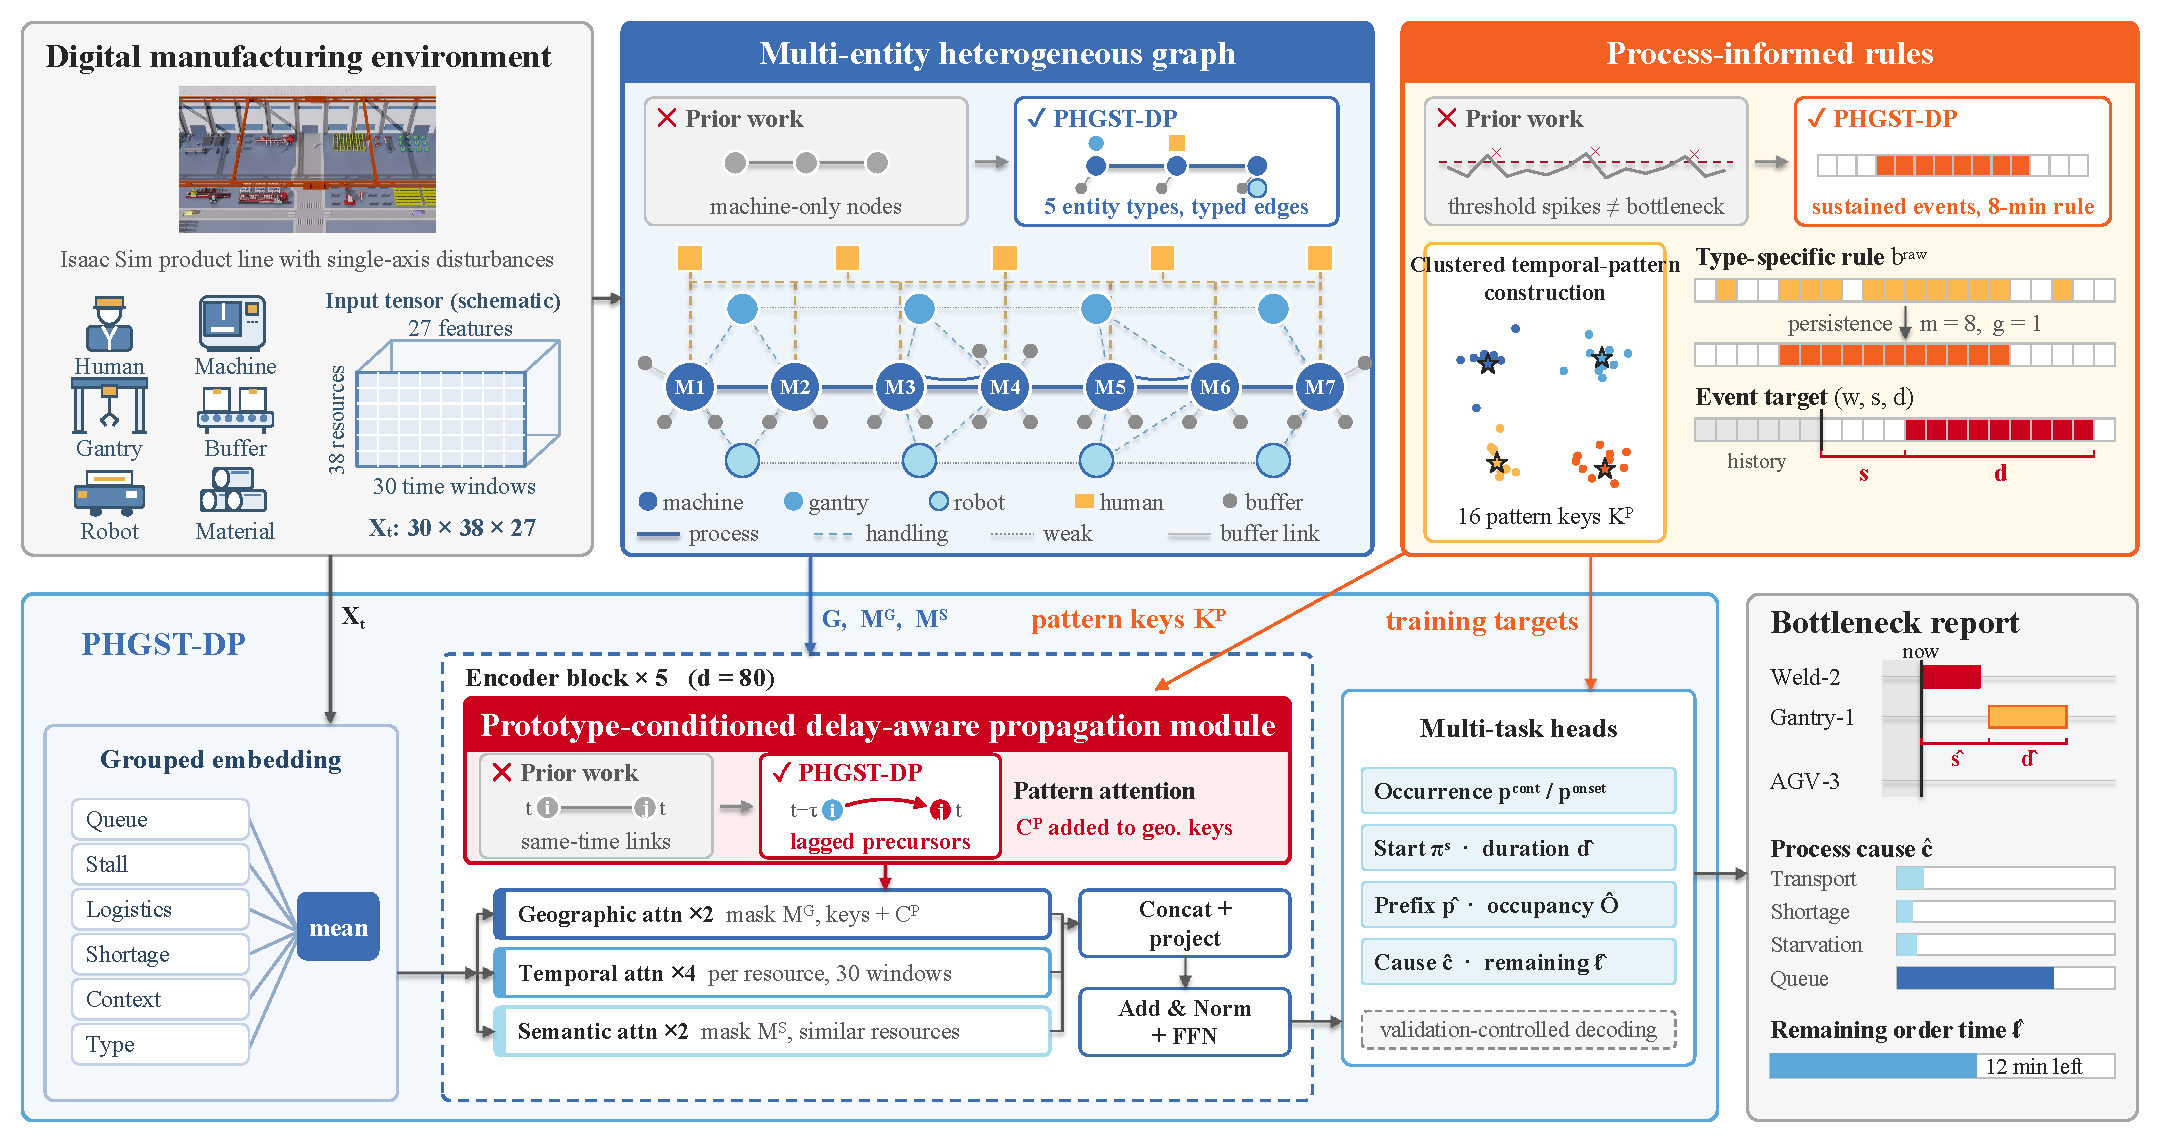
\includegraphics[width=\textwidth]{figures/fig_method_final.pdf}
\caption{Overview of the problem formulation and the PHGST-DM method.}
\label{fig:method-framework}
\end{figure*}

\subsection{Production system and resource relations}

The production system comprises multiple interacting resource entities. We represent this multi-entity environment as a heterogeneous process--logistics graph with resource-specific node types and typed relations. This representation distinguishes the resources that receive bottleneck-event supervision from the contextual resources that influence how constraints form and propagate.

\zhpara{生产系统由多个相互作用的资源实体组成。本文将这一多实体环境表示为具有资源类型节点与带类型关系的异构工艺—物流图。该表示区分接受瓶颈事件监督的资源，以及影响约束形成与传播的上下文资源。}

\subsubsection{Production task and resource entities}

We consider a shared water-pipe production line represented in an open-workspace factory environment, with cutting, grooving, spot welding, root welding, surface welding, and finishing operations. In this study, a workstation denotes a processing or assembly unit, including automated equipment and manually operated workbenches. The process is coupled with storage, gantry handling, transport-robot delivery, and worker service. The graph implementation represents the primary process backbone with seven workstation nodes because parallel workbench and rotary-welding resources are retained as separate stations. Each production episode contains one order of ten products, and the nominal controller admits at most five products as concurrent WIP. It coordinates admission, process precedence, resource availability, and handling tasks; bottleneck prediction observes this controlled process but does not replace the controller.

\zhpara{本文考虑一条共享式数字制造产线，水管产品依次经过切割、开槽、点焊、根部焊接、表面焊接和后处理等工序，并与仓储、龙门搬运、运输机器人配送及人工服务相耦合。图实现将平行工作台和旋转焊接资源分别保留为独立工位，因此主要工艺骨干由七个工作站节点表示。每个生产 episode 包含一个十件产品订单，名义控制器最多允许五件产品同时作为在制品进入系统，并负责任务准入、工艺先后、资源可用性和搬运任务协调。瓶颈预测对这一受控生产过程进行观测，但不取代底层控制器。}

Let the complete resource set be
\begin{equation}
\mathcal{R}=\mathcal{R}^{m}\cup\mathcal{R}^{g}\cup
\mathcal{R}^{a}\cup\mathcal{R}^{h}\cup\mathcal{R}^{b},
\end{equation}
where the superscripts denote workstations, gantries, transport robots, workers, and buffers. The retained graph contains 38 nodes: 7 workstation nodes, 4 gantries, 4 transport robots, 5 workers, and 18 buffers. Material is not represented as a separate graph node; its state enters through shortage propagation, inbound waiting, affiliated-buffer occupancy, and other material-flow channels attached to the affected resources. These entities have different operational meanings. A workstation transforms a product, a gantry or transport robot moves a product between locations, a worker provides labour-dependent service, and a buffer stores intermediate products. The event-supervised target set is
\begin{equation}
\mathcal{S}=\mathcal{R}^{m}\cup\mathcal{R}^{g}\cup\mathcal{R}^{a}.
\end{equation}
Worker and buffer nodes remain in the observation graph because labour availability and storage occupancy influence other resources, but the current implementation does not assign them station-event targets.

\zhpara{记完整资源集合为
\begin{equation}
\mathcal{R}=\mathcal{R}^{m}\cup\mathcal{R}^{g}\cup
\mathcal{R}^{a}\cup\mathcal{R}^{h}\cup\mathcal{R}^{b},
\end{equation}
其中上标分别表示工位、龙门、运输机器人、工人和缓冲区。保留图包含 38 个节点：7 个工位节点、4 个龙门、4 个运输机器人、5 名工人和 18 个缓冲区。物料不作为单独图节点表示；其状态通过短缺传播、入库等待、附属缓冲占用以及其他附着于受影响资源的物料流通道进入模型。这些实体具有不同的运行含义：工位完成产品加工，龙门或运输机器人在位置间搬运产品，工人提供依赖劳动力的服务，缓冲区存放中间产品。事件监督的目标集合为
\begin{equation}
\mathcal{S}=\mathcal{R}^{m}\cup\mathcal{R}^{g}\cup\mathcal{R}^{a}.
\end{equation}
工人与缓冲节点仍保留在观测图中，因为劳动力可用性与存储占用会影响其他资源，但当前实现不为其分配工位事件目标。}

\subsubsection{Heterogeneous process--logistics graph}

The production system is represented as a weighted undirected graph
\begin{equation}
G=(\mathcal{R},E,A),\qquad
E=E^{p}\cup E^{f}\cup E^{b}\cup E^{l}\cup E^{w},
\end{equation}
where $E^{p}$ follows the seven-station process chain, $E^{f}$ connects parallel workstations belonging to the same equipment family, $E^{b}$ links storage buffers to affiliated workstations, $E^{l}$ links handling agents to workstation resources, and $E^{w}$ provides weak links among gantries or among transport robots. The implemented edge weights are $1.0$, $0.8$, $0.6$, $0.5$, and $0.3$ for these five relation groups, respectively, and every node receives a self-loop of weight $1.0$.

\zhpara{生产系统表示为加权无向图
\begin{equation}
G=(\mathcal{R},E,A),\qquad
E=E^{p}\cup E^{f}\cup E^{b}\cup E^{l}\cup E^{w},
\end{equation}
其中 $E^{p}$ 沿七工位工艺链，$E^{f}$ 连接同一设备族中的并联工位，$E^{b}$ 将存储缓冲连接到附属工位，$E^{l}$ 将搬运代理连接到工位资源，$E^{w}$ 在龙门之间或运输机器人之间提供弱连接。上述五类关系的实现边权分别为 $1.0$、$0.8$、$0.6$、$0.5$ 和 $0.3$，且每个节点带有权为 $1.0$ 的自环。}

The graph preserves resource-type distinctions and specifies possible channels through which material flow, service delay, and congestion can propagate. Process edges encode downstream dependency; buffer edges expose storage-mediated blockage or starvation; and logistics edges connect a delayed workstation input to the handling resources that can cause it. This distinction is important because two nodes may be structurally close but have different feature semantics, while two structurally distant nodes may exhibit similar operating trajectories. Section~\ref{sec:method} therefore derives both geographic and semantic attention masks from $G$ and the training trajectories.

\zhpara{该图保留资源类型区分，并规定物料流、服务延迟和拥堵可能传播的通道。工艺边编码下游依赖，缓冲区边揭示由存储引起的阻塞或饥饿，物流边则把延迟的工位入站与可能造成该延迟的搬运资源联系起来。这一区分十分重要：结构相近的节点可能具有不同特征语义，而结构较远的节点也可能呈现相似运行轨迹。因此，第~\ref{sec:method}节将分别从图结构和训练轨迹构建地理注意力与语义注意力掩码。}

\subsection{State representation and prediction targets}

The resource graph is observed through fixed production windows and paired with process-informed event and auxiliary targets. The following definitions align the historical input, future bottleneck interval, process cause, and order-level progress within one prediction sample.

\zhpara{资源图通过固定生产窗口进行观测，并与过程知情事件目标及辅助目标配对。以下定义在同一预测样本中对齐历史输入、未来瓶颈区间、过程原因和订单级进度。}

\subsubsection{Windowed production state}

Raw factory-model events are sampled at logical-second resolution and aggregated into non-overlapping windows of $\Delta=60$\,s. For resource $n$ and window $t$, the state $x_{t,n}\in\mathbb{R}^{27}$ contains twenty-one operational variables, five resource-type indicators, and one labour-saturation context variable. The operational variables cover queue and occupancy, activity and waiting, blockage and starvation, downtime, inter-departure variability, upstream/downstream interaction, route and inbound delay, shortage propagation, affiliated-buffer occupancy, operating variation context, and two turning-point/momentary indicators. Labour saturation is computed from the worker states and broadcast only to workstation nodes. The bottleneck score used by the offline aggregation pipeline is deliberately excluded from $x_{t,n}$ to avoid leaking a supervision signal into the predictor.

\zhpara{原始仿真事件以逻辑秒为分辨率采集，并聚合为互不重叠的 $\Delta=60$ 秒窗口。资源 $n$ 在窗口 $t$ 的状态 $x_{t,n}\in\mathbb{R}^{27}$ 由二十一个运营变量、五个资源类型指示变量和一个人力饱和上下文变量组成。运营变量覆盖队列与占用、活跃与等待、阻塞与饥饿、停机、离开间隔波动、上下游交互、路径与入站延迟、缺料传播、关联缓冲区占用、扰动上下文以及转折点和瞬时瓶颈指示。人力饱和状态由人员节点计算并只广播至机器节点。离线聚合流程中的瓶颈评分被明确排除在 $x_{t,n}$ 之外，以避免监督信号泄漏到预测器输入。}

\begin{table}[pos=t]
\centering
\caption{Semantic groups of the 27-dimensional resource state.}
\label{tab:feature-groups}
\scriptsize
\setlength{\tabcolsep}{3pt}
\renewcommand{\arraystretch}{1.12}
\begin{tabularx}{\columnwidth}{@{}l c >{\raggedright\arraybackslash}X@{}}
\toprule
Group & Dim. & Representative information \\
\midrule
Queue & 4 & Queue length, waiting, occupancy, growth \\
Stall & 6 & Blocked/starved time, stop, availability, coupling \\
Logistics & 4 & Departure variation, route/inbound delay, buffer \\
Shortage & 1 & Material-shortage propagation \\
Context & 7 & Activity, duration, time gap, operating variation, turning state, labour \\
Type & 5 & Workstation, gantry, worker, robot, buffer \\
\bottomrule
\end{tabularx}
\end{table}

Given $T_{\mathrm{in}}=30$ historical windows over $N$ resources, the model input is
\begin{equation}
X_t=\left[x_{\tau,n}\right]_
{\substack{\tau=t-T_{\mathrm{in}},\ldots,t-1\\n=1,\ldots,N}}
\in\mathbb{R}^{T_{\mathrm{in}}\times N\times 27}.
\end{equation}
The future label grid contains $H_{\mathrm{label}}=30$ one-minute windows. Within this grid, the admissible event onset $H_{\mathrm{start}}$ is varied between experimental settings. Separating the thirty-minute label grid from the onset cap allows an event to begin up to fifteen minutes ahead while retaining enough future windows to satisfy the eight-window persistence requirement.

\zhpara{给定覆盖 $N$ 个资源的 $T_{\mathrm{in}}=30$ 个历史窗口，模型输入为
\begin{equation}
X_t=\left[x_{\tau,n}\right]_
{\substack{\tau=t-T_{\mathrm{in}},\ldots,t-1\\n=1,\ldots,N}}
\in\mathbb{R}^{T_{\mathrm{in}}\times N\times 27}.
\end{equation}
未来标签网格包含 $H_{\mathrm{label}}=30$ 个一分钟窗口。在该网格内，允许的事件起点上限 $H_{\mathrm{start}}$ 随实验设置变化。将三十分钟标签网格与起点上限分开，使事件可以提前最多十五分钟开始，同时仍保留足够未来窗口以满足八窗口持续性要求。}

\subsubsection{Process-informed supervision for bottleneck events}

A bottleneck label must distinguish a production-relevant constraint from ordinary activity or travel. For each supervised resource, the implementation first applies a type-dependent rule
\begin{equation}
b^{\mathrm{raw}}_{t,n}=\Phi_{\rho(n)}(x_{t,n},X_t)\in\{0,1\},
\end{equation}
where $\rho(n)$ is the resource type. For a workstation, $\Phi_m$ combines queue accumulation with blocked or starved time, coupled upstream/downstream evidence, shortage propagation, inbound or route delay, downtime, and labour-related waiting. An operating variation flag alone is insufficient: it must coincide with queue, stall, or unavailability evidence. For a gantry, a hot state requires route or inbound delay with stalling, or a stop/unavailable state. For a transport robot, inbound waiting must coincide with stalling, or the robot must be frozen/stopped; normal route travel is not considered a bottleneck.

\zhpara{瓶颈标签必须区分真正影响生产的约束与普通作业或运输活动。对于每个监督资源，代码首先应用资源类型相关规则 $b^{\mathrm{raw}}_{t,n}=\Phi_{\rho(n)}(x_{t,n},X_t)$。对于机器，$\Phi_m$ 将队列积压与阻塞或饥饿时间、上下游耦合证据、缺料传播、入站或路径延迟、停机和劳动力等待结合。单独出现扰动标识不足以形成瓶颈标签，它必须同时伴随队列、停滞或不可用证据。对于龙门，热状态要求路径或入站延迟与停滞同时出现，或者资源处于停止/不可用状态。对于运输机器人，入站等待必须伴随停滞，或机器人处于冻结/停止状态；正常路径运输不被视为瓶颈。}

The raw binary grid is converted into sustained occupancy. In the retained configuration, runs shorter than $m=8$ windows are removed first; an internal cold gap of at most $g=1$ window is then filled when it lies between retained hot regions. Denoting short-run removal by $\mathcal{D}_{m}$ and gap filling by $\mathcal{F}_{g}$, the implemented legacy order is
\begin{equation}
o_{:,n}=\mathcal{F}_{g}\!\left(\mathcal{D}_{m}
\left(b^{\mathrm{raw}}_{:,n}\right)\right).
\end{equation}
This persistence requirement rejects isolated threshold crossings. The occupancy grid $o$ is an offline supervision target. At a forecast origin $t$, the model instead uses a history-only state $h_{t-1,n}$ computed from the observed prefix $x_{0:t,:,:}$, with no observations at or after $t$. Any persistence check used to construct this historical state is evaluated on that prefix only; internal-gap filling cannot use a future hot segment. The historical state is therefore distinct from the retrospective label $o_{t-1,n}$. It should not be confused with the offline event CSV, whose score-event merge can retain a one-window event; PHGST-DM training targets are generated from the operational occupancy grid and use the eight-window criterion.

\zhpara{原始二值网格随后被转换为持续性占用。在最终配置中，首先删除短于 $m=8$ 个窗口的热段；若保留热段之间存在不超过 $g=1$ 个窗口的冷间隙，再将该间隙填补。以 $\mathcal{D}_m$ 表示短段删除、$\mathcal{F}_g$ 表示间隙填补，则代码采用的 legacy 顺序为 $o_{:,n}=\mathcal{F}_{g}(\mathcal{D}_{m}(b^{\mathrm{raw}}_{:,n}))$。该持续性要求用于排除孤立阈值穿越。它不能与离线事件 CSV 的评分事件合并规则混淆：后者可保留一个窗口的事件，而 PHGST-DM 训练目标来自运营占用网格，并采用八窗口条件。}

For a history ending immediately before window $t$, the primary target for station $n$ is
\begin{equation}
y_{t,n}^{\mathrm{evt}}=(w_{t,n},s_{t,n},d_{t,n}),
\end{equation}
where $w_{t,n}$ indicates that an eligible run exists, $s_{t,n}$ is its onset offset, and $d_{t,n}$ is its length within the future grid. If the history-only state $h_{t-1,n}=1$ and the future run begins at offset zero, the event is \emph{ongoing}; its future remainder may be shorter than eight windows because the full event already satisfied persistence before the observation boundary. Otherwise, a run with $s_{t,n}>0$ is \emph{upcoming} and must satisfy the configured minimum duration. If several runs are available for one station, the longest eligible run is selected rather than the earliest run.

\zhpara{对于紧邻窗口 $t$ 之前结束的历史序列，工位 $n$ 的主要目标为事件三元组 $y_{t,n}^{\mathrm{evt}}=(w_{t,n},s_{t,n},d_{t,n})$。其中，$w_{t,n}$ 表示存在满足条件的事件段，$s_{t,n}$ 为开始偏移，$d_{t,n}$ 为其在未来网格中的长度。如果资源在历史最后一个窗口处于热状态，且未来事件从偏移零开始，则该事件定义为进行中事件；由于完整事件已在观测边界之前满足持续性条件，其未来剩余部分可以短于八个窗口。否则，$s_{t,n}>0$ 的事件定义为即将发生事件，并必须满足最短持续时间。当同一工位存在多个候选热段时，选择最长的合格事件，而不是最早事件。}

Algorithm~\ref{alg:targets} consolidates the complete supervision pipeline, from type-dependent state evidence to persistent events, cause targets, regime context, and order-level remaining time. Worker and buffer nodes contribute contextual observations but are omitted from station-event decoding because they are not in $\mathcal{S}$.

\zhpara{算法~\ref{alg:targets} 汇总完整监督流程，从资源类型相关状态证据出发，依次构造持续性事件、原因目标、工况上下文和订单层剩余时间。人员和缓冲区提供上下文观测，但不属于 $\mathcal{S}$，因此不参与工位事件解码。}

\begin{algorithm*}[t]
\caption{Process-informed supervision and regime-context construction.}
\label{alg:targets}
\KwIn{episode trajectories $\mathcal{E}$; resource types $\rho$; supervised set $\mathcal{S}$; $T_{\mathrm{in}}$; $H_{\mathrm{label}}$; $H_{\mathrm{start}}$; $m{=}8$; $g{=}1$}
\KwOut{causal samples $\mathcal{D}=\{X_t,O_t,Y_t^{\mathrm{evt}},c_t,\ell_t,r_t\}$}
$\mathcal{D}\leftarrow\varnothing$\;
\ForEach{completed, reset-free episode $e\in\mathcal{E}$}{
  \tcp{Stage 1: synchronize heterogeneous observations}
  aggregate raw streams into non-overlapping $60$,s windows\;
  align resource states by identifier and append type/context channels\;
  preserve the episode boundary and compute jobs remaining\;
  \tcp{Stage 2: construct the persistent occupancy grid}
  \ForEach{$n\in\mathcal{S}$ and window $u$}{
    $b^{\mathrm{raw}}_{u,n}\leftarrow\Phi_{\rho(n)}(x_{u,n})$ using queue, stall, availability, shortage, and logistics evidence\;
  }
  \ForEach{$n\in\mathcal{S}$}{
    $o_{:,n}\leftarrow\mathcal{F}_{g}(\mathcal{D}_{m}(b^{\mathrm{raw}}_{:,n}))$ \tcp*{drop short runs, then fill gaps}
  }
  \tcp{Stage 3: derive process cause and regime context}
  \ForEach{window $u$ and resource $n$}{
    assign $r_{u,n}$ by the deterministic cause-aligned state rules\;
  }
  \ForEach{window $u$ containing reportable hot evidence}{
    assign $c_u$ by the priority shortage $\succ$ delay $\succ$ queue $\succ$ blockage\;
    set the cause-loss weight to $1$ only when $c_u\in\mathcal{C}$\;
  }
  \tcp{Stage 4: instantiate one causal forecasting sample}
  \For{$t\leftarrow T_{\mathrm{in}}$ \KwTo episode completion}{
    $X_t\leftarrow x_{t-T_{\mathrm{in}}:t,:,:}$ and $O_t\leftarrow o_{t:t+H_{\mathrm{label}},:}$\;
    compute $h_{t-1}$ from the observed prefix $x_{0:t,:,:}$ only \tcp*{no retrospective occupancy supplied to inference}
    \ForEach{$n\in\mathcal{S}$}{
      $(s,d)\leftarrow$ longest hot run of $O_{t,:,n}$ whose onset is within $H_{\mathrm{start}}$\;
      \eIf{$h_{t-1,n}=1$ and $s=0$}{
        $(w_{t,n},s_{t,n},d_{t,n})\leftarrow(1,0,d)$ \tcp*{ongoing remainder}
      }{
        \eIf{$0<s\le H_{\mathrm{start}}$ and $d\ge m$}{
          $(w_{t,n},s_{t,n},d_{t,n})\leftarrow(1,s,d)$ \tcp*{upcoming event}
        }{
          $(w_{t,n},s_{t,n},d_{t,n})\leftarrow(0,0,0)$\;
        }
      }
    }
    $\ell_t\leftarrow$ future one-minute windows until all jobs finish, clipped by the prediction cap\;
    append $(X_t,O_t,Y_t^{\mathrm{evt}},c_{t-1},\ell_t,r_{t-1})$ to $\mathcal{D}$\;
  }
}
\Return $\mathcal{D}$\;
\end{algorithm*}

\subsubsection{Cause and order-level targets}

Station events identify where and when production is constrained, but intervention also requires a process explanation. The aggregation pipeline assigns a window-level cause through a fixed evidence priority: material shortage, transport delay, queue buildup, and downstream blockage. The label is inferred from measured shortage, inbound/route delay, queue, and blocked variables; it is not copied from the injected operating variation dimension.

\zhpara{工位事件说明生产约束发生在何处以及何时发生，但生产干预还需要过程解释。聚合流程按照固定证据优先级赋予窗口级原因：物料短缺、运输延迟、队列积压、下游阻塞、上游饥饿和高利用率。该标签依据缺料、入站/路径延迟、队列、阻塞、饥饿和活跃变量推导，而不是复制注入扰动维度。因此，例如机器扰动在传播之后可以形成下游饥饿标签。}

The reported cause set is
\begin{equation}
\begin{aligned}
\mathcal{C}=\{&
\text{material shortage},\text{transport delay},\\
&\text{queue buildup},\text{downstream blockage}\}.
\end{aligned}
\end{equation}
The order-level target $\ell_t$ is the number of future one-minute windows until all jobs are complete under the configured prediction cap. It provides a line-level estimate of production consequence that complements the station-level event report.

\zhpara{报告原因集合为
\begin{equation}
\begin{aligned}
\mathcal{C}=\{&
\text{material shortage},\text{transport delay},\\
&\text{queue buildup},\text{downstream blockage}\}.
\end{aligned}
\end{equation}
订单级目标 $\ell_t$ 是在所配置预测上限下、距全部作业完成尚剩的未来一分钟窗口数。它提供对生产后果的产线级估计，用以补充工位级事件报告。}

The cause-assignment stage of Algorithm~\ref{alg:targets} applies this priority to each reportable hot window. The same algorithm distinguishes these cause targets from deterministic regime identifiers: the former supervise the graph-level explanation head, whereas the latter only condition the station-event representation.

\zhpara{算法~\ref{alg:targets} 的原因分配阶段把上述优先级应用到每个具有可报告热状态证据的窗口。不属于 $\mathcal{C}$ 的标签仍可记录，但在原因损失中权重为零。该算法同时区分原因目标与确定性工况标识：前者监督图级解释头，后者只用于调节工位事件表示。}

\subsection{Multi-task prediction formulation}

The complete prediction problem is the mapping
\begin{equation}
f_{\theta}:(X_t,G)\longmapsto
\left(
\{\hat w_{t,n},\hat s_{t,n},\hat d_{t,n}\}_{n\in\mathcal{S}},
\hat c_t,\hat\ell_t
\right).
\end{equation}
This formulation differs from forecasting a bottleneck score. The outputs jointly describe the affected resource, event onset and persistence, process explanation, and expected order impact. The method in Section~\ref{sec:method} parameterizes $f_{\theta}$ with a delay-aware heterogeneous spatiotemporal encoder and multiple task heads.

\zhpara{完整预测问题被定义为从历史状态与工厂图到所有监督工位事件、过程原因和订单剩余时间的映射。该形式不同于瓶颈评分预测：输出在统一的决策接口中明确给出受影响资源、事件起点、持续性、过程解释和预期订单影响。第~\ref{sec:method}节使用延迟感知异构时空编码器及多任务预测头参数化该映射。}

The delayed-propagation challenge is contained in this mapping rather than introduced as an additional label. For an upcoming event at target resource $j$, predictive evidence may occur at another resource $i$ and at an earlier history offset $\tau$. The model must therefore learn associations of the form
\begin{equation}
(x_{t-\tau,i},\,i\!\rightarrow\!j)\longmapsto y^{\mathrm{evt}}_{t,j},
\qquad \tau>0,
\end{equation}
where $i\!\rightarrow\!j$ denotes a possible process or logistics route, not a proven physical causal path. This formulation motivates conditioning cross-resource interaction on recurrent historical patterns while evaluating success only through the future event report.

\zhpara{延迟传播困难包含在上述映射中，而不是通过额外标签引入。对于目标资源 $j$ 的 upcoming 事件，可预测证据可能出现在另一资源 $i$ 及更早的历史偏移 $\tau$ 处。因此，模型需要学习从较早资源状态与可能的工艺或物流路径到未来目标事件的关联。这里的 $i\!\rightarrow\!j$ 表示潜在传播通道，而不是已经证明的物理因果路径。该形式化为“使用重复历史模式调节跨资源交互”提供动机，而模型成败仍只通过未来事件报告进行评价。}

Two event criteria are distinguished. A station-level hit requires that the predicted resource equal the labelled resource. A stricter report-level true positive additionally requires
\begin{equation}
|\hat{s}_{t,n}-s_{t,n}|\leq\epsilon_s,\qquad
\epsilon_s=3~\mathrm{min}.
\end{equation}
Occurrence precision, recall, and F1 quantify the coverage and reliability of alarms. Start, duration, and remaining-time errors are conditional or regression measures and cannot compensate for a missed station event. Ongoing and upcoming recalls are therefore reported separately: the latter is the direct measure of whether the model provides warning before the bottleneck becomes visible at the target station.

\zhpara{本文区分两种事件判定标准。工位级命中要求预测资源与标签资源一致；更严格的报告级真阳性还要求开始时间误差不超过 $\epsilon_s=3$ 分钟。事件精确率、召回率和 F1 衡量报警的可靠性与覆盖程度；开始时间、持续时间和订单剩余时间误差属于条件性或回归指标，不能弥补工位事件漏检。因此，本文分别报告进行中与即将发生事件的召回率，其中后者直接衡量模型能否在瓶颈于目标工位显现之前提供预警。}

%% ========================================================================
\section{Methodology} \label{sec:method}
%% ========================================================================

\subsection{Method overview}

PHGST-DM is organized around the three contributions established in Section~\ref{sec:intro}. First, an open-workspace factory model developed for NVIDIA Isaac Sim, a heterogeneous factory graph, and grouped embedding integrate workstation, worker, material-flow, buffer, gantry, and transport evidence. Second, process-informed supervision and temporal pattern clustering produce traceable event and cause supervision, deterministic regime context, and recurrent operating-pattern prototypes. Third, delay-aware spatiotemporal modeling uses those prototypes to organize lagged cross-resource interaction. The complete information flow is
\begin{equation}
\begin{aligned}
\text{factory model}&\rightarrow\text{window/event construction}\\
&\rightarrow\text{factory graph}\rightarrow\text{joint prediction}.
\end{aligned}
\end{equation}
The first two stages create reproducible observations and targets. The latter two parameterize the mapping $f_\theta$ defined in Section~\ref{sec:problem}.

\zhpara{PHGST-DM 围绕第~\ref{sec:intro}节确立的三项贡献组织。第一，面向 NVIDIA Isaac Sim 开发的开放式工厂模型、异构工厂图与分组嵌入，整合工位、工人、物料流、缓冲、龙门与运输证据。第二，过程知情监督与时间模式聚类产生可追溯的事件与原因监督、确定性工况上下文以及重复运行模式原型。第三，延迟感知建模利用这些原型组织滞后的跨资源交互。完整信息流为
\begin{equation}
\begin{aligned}
\text{factory model}&\rightarrow\text{window/event construction}\\
&\rightarrow\text{factory graph}\rightarrow\text{joint prediction}.
\end{aligned}
\end{equation}
前两阶段形成可复现的观测与目标；后两阶段参数化第~\ref{sec:problem}节定义的映射 $f_\theta$。}

Figure~\ref{fig:model-architecture} presents the PHGST-DM model architecture. The multi-entity history is partitioned into six semantic feature groups and combined with temporal, graph-Laplacian, and node-identity embeddings. Temporal pattern clustering supplies a fixed prototype bank, and delay-aware spatiotemporal modeling uses that bank to condition geographic keys so that recurrent precursors can influence cross-resource interaction after a delay. Station-level and graph-level heads then decode occurrence, onset, duration, future occupancy, process cause, and remaining order time.

\zhpara{图~\ref{fig:model-architecture}给出 PHGST-DM 的模型结构。多实体历史被划分为六个语义特征组，并与时间、图拉普拉斯与节点身份嵌入相结合。时间模式聚类提供固定原型库；延迟感知建模利用该库调节地理键，使重复出现的前驱模式能在延迟后影响跨资源交互。随后，工位级与图级输出头解码发生与否、开始时间、持续时间、未来占用、过程原因以及订单剩余时间。}

\begin{figure*}[t]
\centering
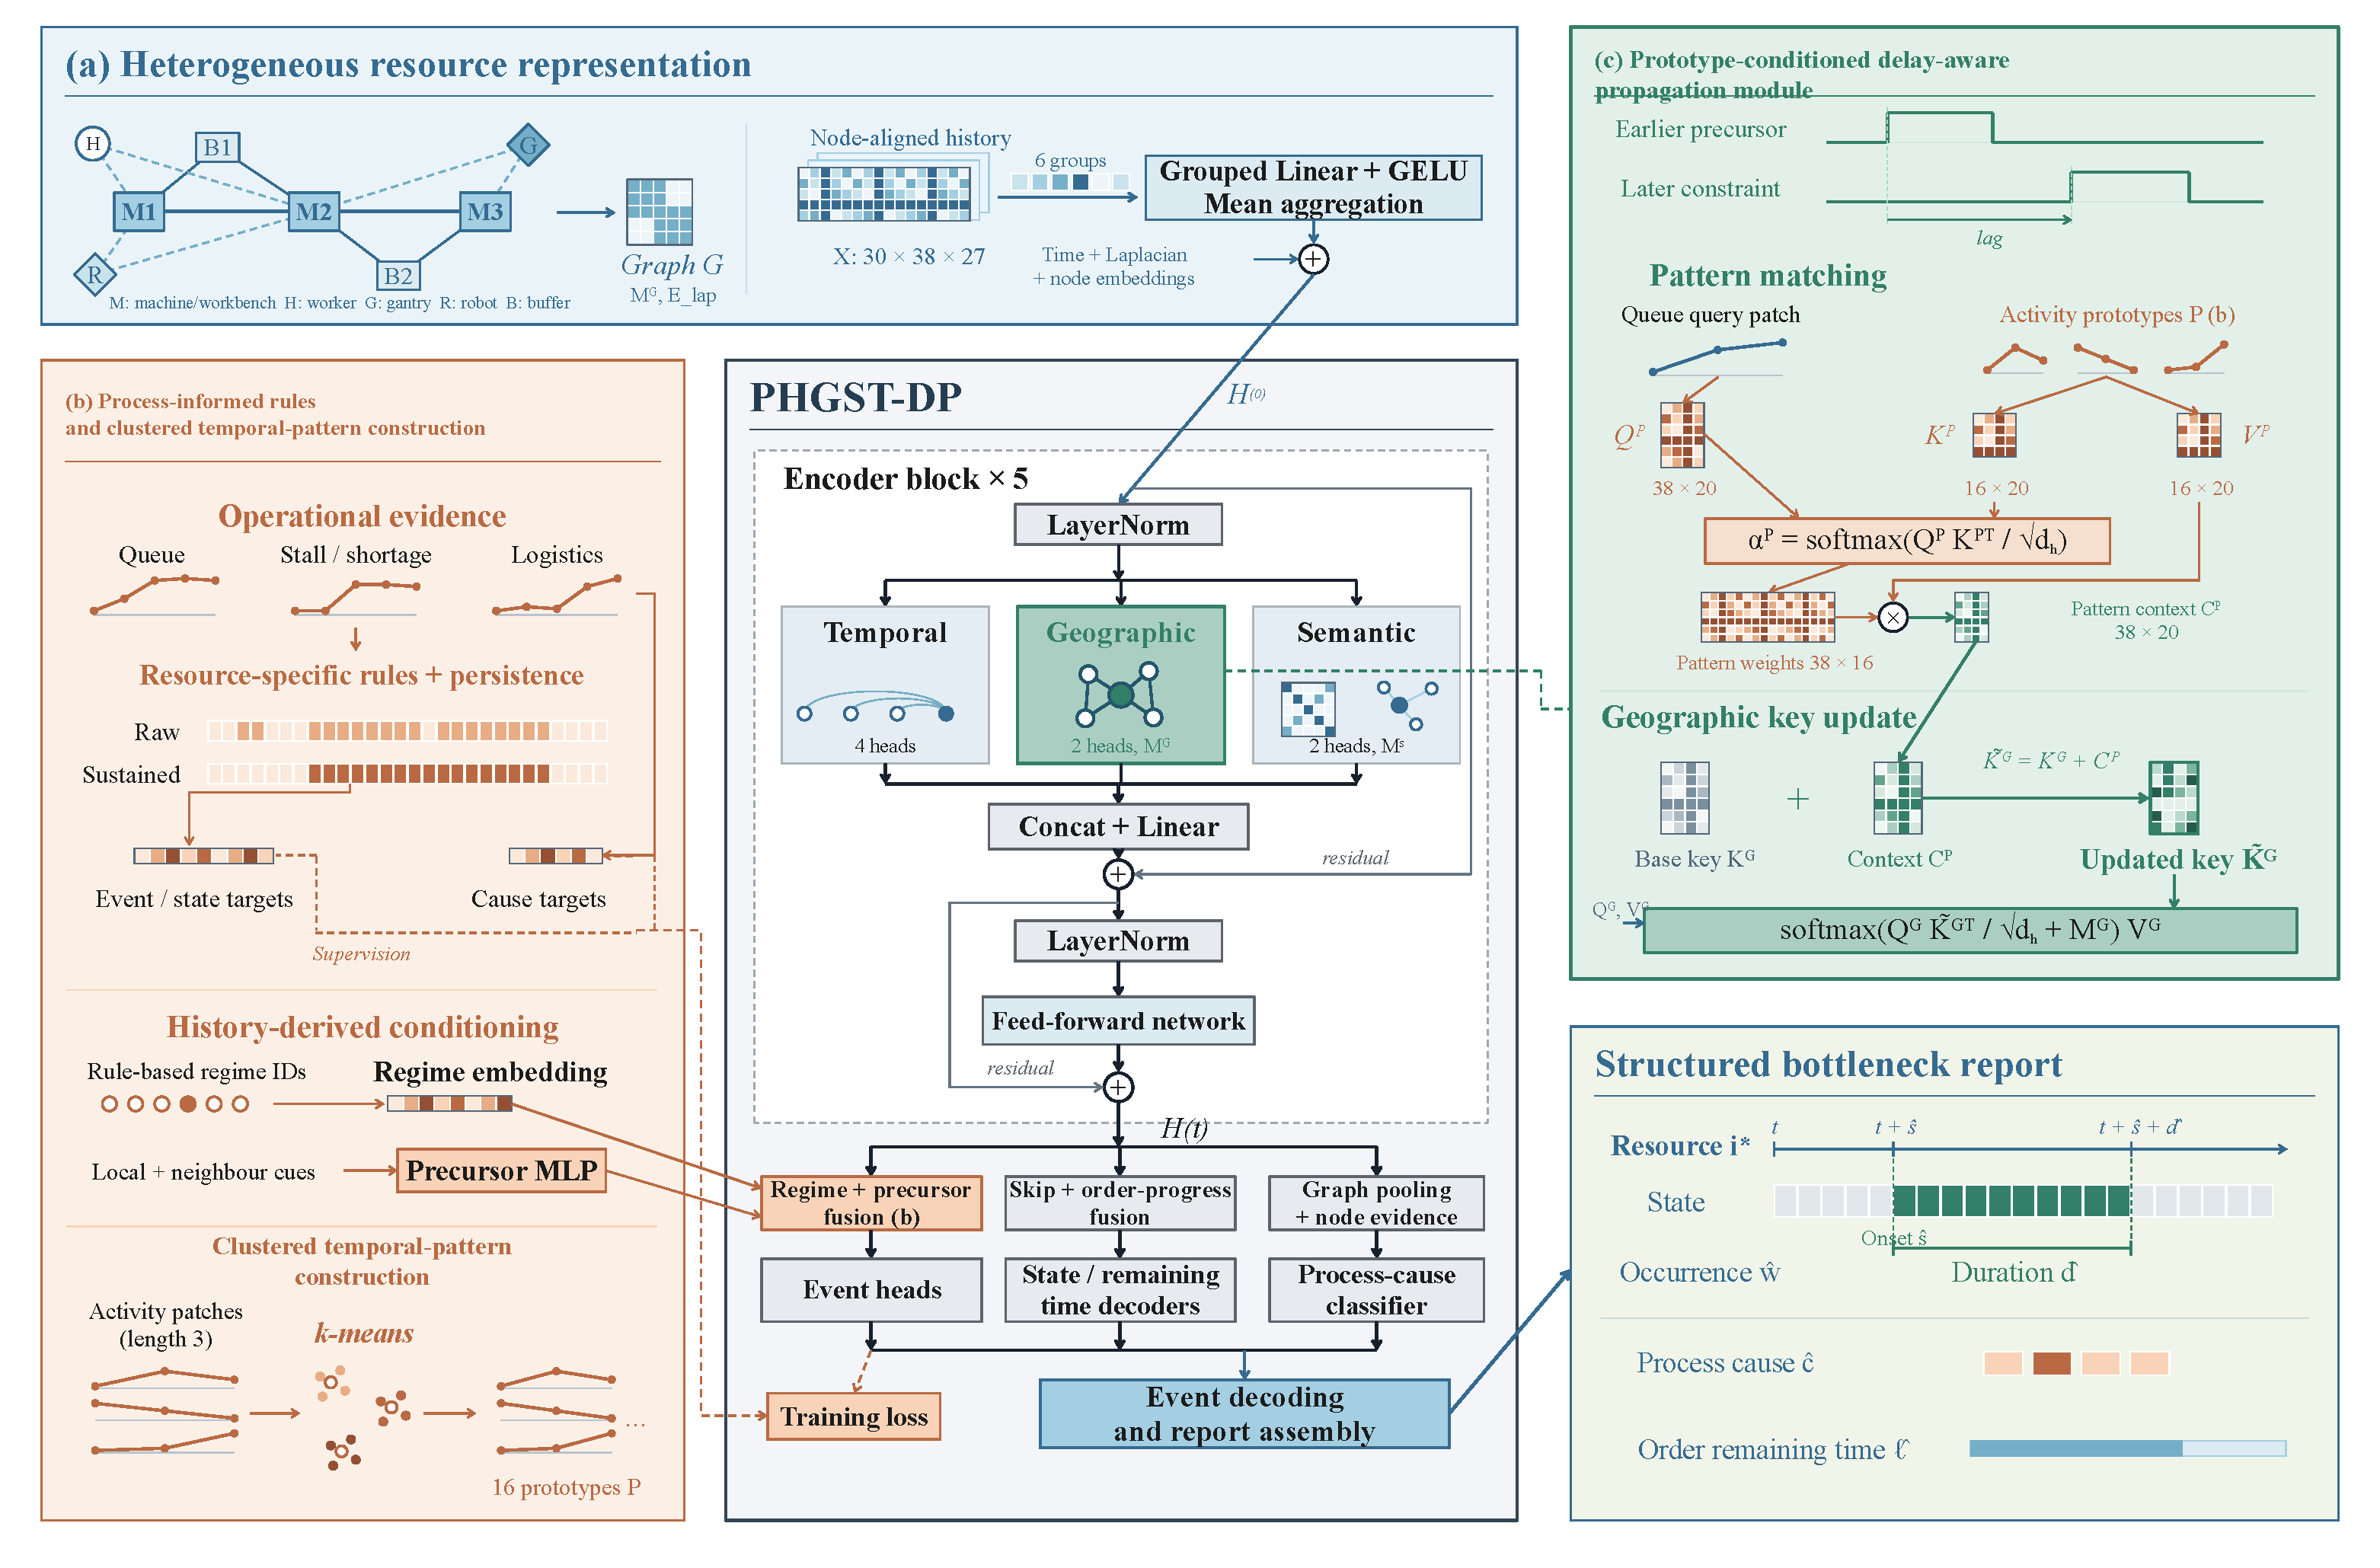
\includegraphics[width=\textwidth]{figures/fig_model_final.pdf}
\caption{Architecture of PHGST-DM.}
\label{fig:model-architecture}
\end{figure*}

Algorithm~\ref{alg:phgst-train} gives the end-to-end learning and model-selection procedure around that architecture. It makes explicit which quantities are fitted from training episodes, how validation controls checkpoint and threshold selection, and when the held-out episodes are first evaluated. Algorithm~\ref{alg:phgst-predict} then expands one complete PHGST-DM forward and report-generation pass.

\zhpara{算法~\ref{alg:phgst-train} 给出围绕该架构的端到端学习与模型选择过程，明确区分由训练 episode 拟合的量、由验证集控制的 checkpoint 与阈值选择，以及留出测试 episode 首次参与评价的时点。算法~\ref{alg:phgst-predict} 随后展开一次完整的 PHGST-DM 前向计算与报告生成过程。}

\begin{algorithm*}[t]
\SetAlFnt{\small}
\SetAlCapFnt{\small}
\SetAlCapNameFnt{\small\bfseries}
\SetInd{0.6em}{1.0em}
\caption{End-to-end PHGST-DM training, selection, and held-out evaluation.}
\label{alg:phgst-train}
\KwIn{raw episodes $\mathcal{E}$; factory relations $G$; onset caps $\mathcal{H}=\{5,10,15\}$; candidate thresholds $\mathcal{T}$}
\KwOut{frozen event model $\theta^{\star}$, remaining-time head $\psi^{\star}$, threshold $\tau^{\star}$, held-out reports}
\BlankLine
\textbf{Stage 1: leakage-controlled data and fixed structural context}\;
split $\mathcal{E}$ by episode into $\mathcal{E}_{\mathrm{tr}},\mathcal{E}_{\mathrm{val}},\mathcal{E}_{\mathrm{te}}$\;
construct causal samples with Algorithm~\ref{alg:targets} independently inside each episode\;
fit all feature/target scalers on $\mathcal{E}_{\mathrm{tr}}$; reuse them unchanged for $\mathcal{E}_{\mathrm{val}}$ and $\mathcal{E}_{\mathrm{te}}$\;
obtain $(A,M^{G},M^{S},E_{\mathrm{lap}})$ from Algorithm~\ref{alg:graph-masks} and $K^{P}$ from Algorithm~\ref{alg:pattern-bank}\;
freeze every data-derived structural quantity before neural-parameter optimization \tcp*{masks and prototypes stay fixed}
\BlankLine
\textbf{Stage 2: curriculum learning of shared representations and event-related heads}\;
initialize $\theta$ from the documented prefix-supervised checkpoint\;
\ForEach{$H_{\mathrm{start}}\in\mathcal{H}$ in curriculum order}{
  warm-start the current onset cap from the preceding retained checkpoint when available\;
  \For{epoch $=1,\ldots,E_1$ until patience is exhausted}{
    \ForEach{oversampled training minibatch $B$}{
      $(\widehat{Y}^{\mathrm{evt}},\hat O,\hat c,\hat\ell)\leftarrow\mathrm{PHGSTDMForward}_{\theta}(B,A,M^{G},M^{S},K^{P})$\;
      evaluate the event, occupancy, cause, reconstruction, contrastive, and remaining-time losses, then update $\theta$\;
    }
    decode $\mathcal{E}_{\mathrm{val}}$ with Algorithm~\ref{alg:phgst-predict} for every $\tau\in\mathcal{T}$\;
    retain the checkpoint--threshold pair that passes the precision/recall gates and maximizes station F1\;
  }
}
freeze the selected stage-1 parameters and threshold as $(\theta^{\star},\tau^{\star})$ \tcp*{event reports locked hereafter}
\BlankLine
\textbf{Stage 3: remaining-time specialization without changing event reports}\;
freeze the encoder and all event, occupancy, and cause heads\;
initialize the rate-augmented remaining-time head $\psi$ from $\theta^{\star}$\;
\For{epoch $=1,\ldots,E_2$ until validation loss stops improving}{
  update only $\psi$ using progress-weighted remaining-time loss\;
}
freeze $\psi^{\star}$; do not retune $\tau^{\star}$\;
\BlankLine
\textbf{Stage 4: held-out evaluation after all choices are frozen}\;
run Algorithm~\ref{alg:phgst-predict} on $\mathcal{E}_{\mathrm{te}}$ using $(\theta^{\star},\psi^{\star},\tau^{\star})$\;
\Return frozen models, threshold, and held-out reports \tcp*{test episodes never re-enter selection}
\end{algorithm*}

\subsection{Data preparation and graph instantiation}

Section~\ref{sec:problem} defines the entities, graph relations, and prediction targets. This stage describes only how those formal objects are instantiated for PHGST-DM: factory-model trajectories are converted into a synchronized resource--time tensor, aligned supervision targets, and the structural and semantic masks required by the encoder.

\zhpara{第~\ref{sec:problem}节已经定义实体、图关系与预测目标，本节仅说明这些形式化对象如何在 PHGST-DM 中实例化：将可追溯的受控扰动轨迹转换为同步资源—时间张量、对齐的监督目标以及编码器所需的结构与语义掩码。}

\subsubsection{Open-workspace factory model}

Data are collected using an open-workspace factory model developed for NVIDIA Isaac Sim. The model represents the water-pipe line, resource layout, storage locations, and handling activities. At every logical second, the collector records the episode configuration, active operating variation, resource-state transitions, job traces, buffer events, transport tasks, and material inventory. These streams are synchronized by episode and logical time, allowing a downstream event to be traced back through the states that preceded it. A known model implementation defect can trigger a deadlock reset that is not part of the intended production process and does not represent a physical production condition. Episodes affected by this defect are treated as invalid model records and removed; valid episodes are exported after all ten products complete.

\zhpara{数据利用面向 NVIDIA Isaac Sim 开发的开放式工厂模型采集。该模型表示水管产线、资源布局、仓储位置与搬运活动。采集器在每个逻辑秒记录 episode 配置、活动运行变化、资源状态转移、作业轨迹、缓冲事件、运输任务与物料库存。这些数据流按 episode 与逻辑时间对齐，从而使下游事件能够回溯到其前序状态。已知的模型实现缺陷可能触发并非预期生产过程、也不代表实体生产条件的死锁复位；受该缺陷影响的 episode 被视为无效模型记录并剔除，有效 episode 在十件产品全部完成后导出。}

Formal single-axis collection activates one operating variation dimension at intensity $I=1.0$ while leaving the other dimensions nominal:
\begin{itemize}
 \item[$\bullet$] \textbf{Workstation operating variation} increases processing-time variation, lowers successful operation probability, disables selected workstations, and inserts temporary workstation-fault pulses.
 \item[$\bullet$] \textbf{Worker operating variation} reduces the workforce from five to three, increases task-time variation, and inserts temporary leave periods.
 \item[$\bullet$] \textbf{Logistics operating variation} reduces transport robots from four to two, slows gantry motion, and inserts handling freezes that include an AGV freeze.
 \item[$\bullet$] \textbf{Material operating variation} temporarily hides flange or elbow kits and introduces additional shortage pulses for selected stock-keeping units.
\end{itemize}
The temporary workstation, worker, and logistics pulses last at least ten logical minutes. This design does not assume that the injected dimension is the final bottleneck cause. Its purpose is to produce traceable perturbations whose operational consequences can emerge at different resources and times.

\zhpara{正式单轴采集在强度 $I=1.0$ 下激活一个运行变化维度，其余维度保持名义条件：
\begin{itemize}
 \item[$\bullet$] \textbf{工位运行变化}增大加工时间波动、降低成功操作概率、停用选定工位，并插入临时工位故障脉冲。
 \item[$\bullet$] \textbf{工人运行变化}将劳动力从五人减至三人、增大任务时间波动，并插入临时离岗时段。
 \item[$\bullet$] \textbf{物流运行变化}将运输机器人从四台减至两台、减慢龙门运动，并插入包含 AGV 冻结在内的搬运冻结。
 \item[$\bullet$] \textbf{物料运行变化}临时隐藏法兰或弯头套件，并对选定库存单元引入额外短缺脉冲。
\end{itemize}
临时工位、工人与物流脉冲至少持续十个逻辑分钟。该设计并不假定所注入维度即为最终瓶颈原因；其目的是产生可追溯扰动，使其运行后果可在不同资源与时刻显现。}

\subsubsection{Multi-entity aggregation and target instantiation}

The second stage converts heterogeneous raw logs into a common resource--time grid. Statistics are aggregated over non-overlapping one-minute windows and aligned by resource identifier. Missing resource states are completed through the export pipeline, type one-hot variables are appended, and labour saturation is recomputed from the available worker nodes. The resulting tensor contains 38 resource nodes and 27 channels in the retained dataset. Episode boundaries are preserved throughout sliding-window generation, preventing a history from combining observations from two production runs.

\zhpara{第二阶段将异构原始日志转换为统一的资源—时间网格。统计量按互不重叠的一分钟窗口聚合并依据资源标识对齐；缺失资源状态由导出流程补齐，随后加入类型独热变量，并依据可用人员节点重新计算人力饱和状态。最终保留数据集包含三十八个资源节点和二十七个通道。滑动窗口生成过程中始终保留 episode 边界，避免一个历史样本拼接两个不同生产运行。}

The pipeline instantiates the supervision defined in Section~\ref{sec:problem} from each aggregated episode, producing aligned occurrence, onset, duration, occupancy-grid, prefix, process-cause, and remaining-time targets. The retained configuration derives event targets from operational states rather than the exported bottleneck-score column, preventing the model from solving the task by reproducing an aggregation score.

\zhpara{数据流程依据第~\ref{sec:problem}节的定义，从每个聚合 episode 实例化彼此对齐的事件发生、起点、持续时间、未来占用网格、prefix、过程原因和订单剩余时间目标。最终配置依据运营状态生成事件目标，而不使用导出的瓶颈评分列，从而避免模型通过复现聚合评分完成任务。}

Three different clustering-related objects are kept conceptually separate. First, the offline aggregation tools can produce station- and window-level $K=8$ k-means descriptors for exploratory regime analysis. Second, the training dataset derives cause-aligned regime identifiers by deterministic rules and can use them for representation conditioning and contrastive regularization. Third, the temporal pattern clustering component fits short temporal patches to create the recurrent prototype bank. Temporal pattern clustering fits the prototype bank. Delay-aware spatiotemporal modeling then matches recent patches to these prototypes and adds the resulting context to geographic attention. The offline cluster-prediction loss has weight zero, and no cluster index defines the bottleneck ground truth; event labels are produced only by the process rules and persistence filter above.

\zhpara{与聚类相关的三类对象在概念上保持分离。第一，离线聚合工具可生成工位级与窗口级的 $K=8$ k-means 描述子，用于探索性工况分析。第二，训练数据由确定性规则导出原因对齐的工况标识，并可用于表示条件化与对比正则。第三，时间模式聚类组件将短时片段拟合为重复原型库。时间模式聚类负责拟合该原型库；延迟感知建模再将近期片段与这些原型匹配，并把所得上下文加入地理注意力。离线聚类预测损失权重为零，且不以簇索引作为瓶颈真值；事件标签仅由上述过程规则与持续性过滤生成。}

\subsubsection{Heterogeneous factory graph and attention masks}

The weighted adjacency $A$ follows the relation definitions in Section~\ref{sec:problem}. Floyd--Warshall shortest-path computation converts nonzero edges into hop distances $D^{\mathrm{hop}}$. The geographic mask is
\begin{equation}
M^G_{ij}=
\begin{cases}
0, & D^{\mathrm{hop}}_{ij}<\delta_G,\\
-\infty, & \text{otherwise},
\end{cases}
\qquad \delta_G=4,
\end{equation}
so a node attends only to resources fewer than four hops away in geographic attention. This mask allows information to cross more than one process or logistics edge while excluding globally unrelated nodes.

\zhpara{加权邻接矩阵 $A$ 遵循第~\ref{sec:problem}节的关系定义。Floyd--Warshall 最短路径计算将非零边转换为跳数距离 $D^{\mathrm{hop}}$。地理掩码仅允许最短路径小于 $\delta_G=4$ 的节点相互注意，使信息可以跨越不止一条工艺或物流边传播，同时排除全局无关节点。}

Geographic proximity alone cannot capture parallel or substitutable resources with similar behaviour. A semantic distance matrix is therefore computed from training trajectories. The feature channels of each node are first averaged to form a scalar trajectory $\bar x_{:,i}$, after which
\begin{equation}
D^{\mathrm{sem}}_{ij}
=1-\mathrm{corr}(\bar{x}_{:,i},\bar{x}_{:,j}).
\end{equation}
For each node, the five nearest trajectories are unmasked in $M^S$; all others are suppressed. This implementation uses Pearson correlation distance as a short-episode substitute for the dynamic-time-warping distance used in traffic PDFormer. Finally, the nontrivial eigenvectors of the normalized graph Laplacian provide an eight-dimensional structural position for every resource. The exact graph-and-mask instantiation invoked during training is isolated in Algorithm~\ref{alg:graph-masks}. All trajectory-dependent quantities in this procedure are computed from the training split only.

\zhpara{仅依赖地理邻近无法表示行为相似的平行或可替代资源，因此模型还依据训练轨迹构建语义距离矩阵。首先对每个节点的特征通道取平均形成标量轨迹 $\bar x_{:,i}$，再计算 $D^{\mathrm{sem}}_{ij}=1-\mathrm{corr}(\bar{x}_{:,i},\bar{x}_{:,j})$。对于每个节点，语义掩码 $M^S$ 仅保留距离最近的五条轨迹。该实现以 Pearson 相关距离替代交通 PDFormer 中适合长交通序列的动态时间规整距离。最后，归一化图拉普拉斯的非平凡特征向量为每个资源提供八维结构位置。训练阶段调用的完整图与掩码实例化过程见算法~\ref{alg:graph-masks}，其中所有依赖轨迹的量均只由训练集计算。}

\subsection{Delay-aware heterogeneous spatiotemporal encoding}

The encoder first preserves the distinct semantics of heterogeneous observations through grouped embedding and then models temporal evolution, graph propagation, and behavioural similarity. Delay-aware spatiotemporal modeling further links current resource states with recurrent precursor patterns whose effects emerge later in the production process.

\zhpara{编码器首先通过分组嵌入保留异构观测的不同语义，随后联合建模时间演化、图上传播和资源行为相似性。延迟感知建模进一步将当前资源状态与生产过程中后续显现影响的重复前驱模式联系起来。}

\subsubsection{Grouped heterogeneous state embedding}

A single linear projection would combine all 27 channels without explicitly distinguishing the semantics of queue length, downtime, type codes, and shortage evidence. The grouped token embedding instead partitions the channels into queue, stall, logistics, shortage, context, and type groups. Each group $q$ has an independent affine projection and GELU activation:
\begin{equation}
e^{(q)}_{t,n}=\mathrm{GELU}
\left(W_q x^{(q)}_{t,n}+b_q\right).
\end{equation}
The six group embeddings are mean-pooled, rather than concatenated as separate tokens:
\begin{equation}
e_{t,n}=\frac{1}{6}\sum_{q=1}^{6}e^{(q)}_{t,n}.
\end{equation}
This operation maps heterogeneous evidence to a common latent space and gives each feature group equal weight in the pooling step, regardless of its channel count.

\zhpara{若用单一线性投影合并全部 27 个通道，将无法显式区分队列长度、停机、类型编码与短缺证据等语义。分组标记嵌入则将通道划分为队列、停滞、物流、短缺、上下文与类型六组。每一组 $q$ 使用独立仿射投影与 GELU 激活：
\begin{equation}
e^{(q)}_{t,n}=\mathrm{GELU}
\left(W_q x^{(q)}_{t,n}+b_q\right).
\end{equation}
六组嵌入取均值池化，而不是拼接为独立标记：
\begin{equation}
e_{t,n}=\frac{1}{6}\sum_{q=1}^{6}e^{(q)}_{t,n}.
\end{equation}
该操作将异构证据映射到共同潜空间，并在池化步中使各组权重相等，而不依赖其通道数量。}

The initial representation combines grouped evidence with temporal, structural, and identity information:
\begin{equation}
H^{(0)}=E_{\mathrm{group}}(X_t)+
E_{\mathrm{time}}+E_{\mathrm{lap}}(G)+E_{\mathrm{node}}.
\end{equation}
$E_{\mathrm{time}}$ is sinusoidal, $E_{\mathrm{lap}}$ projects the graph eigenvectors, and $E_{\mathrm{node}}$ is a learned resource-identity embedding. Day-of-week and time-of-day embeddings are disabled because an episode is driven by order progress and operating variations rather than calendar periodicity.

\zhpara{初始表示由分组证据、时间信息、图结构和节点身份共同组成。$E_{\mathrm{time}}$ 为正弦时间位置编码，$E_{\mathrm{lap}}$ 投影图拉普拉斯特征向量，$E_{\mathrm{node}}$ 为可学习资源身份嵌入。模型关闭星期和日内时刻编码，因为 episode 演化由订单进度和扰动驱动，而不是由日历周期驱动。}

\subsubsection{Delay-aware spatiotemporal modeling}

Delay-aware spatiotemporal modeling must distinguish three dependencies: evolution of one resource through time, propagation through the process--logistics graph, and similarity between resources that need not be adjacent. Each encoder block therefore allocates separate attention heads to temporal, geographic, and semantic attention. For an attention branch $b\in\{T,G,S\}$,
\begin{equation}
\mathrm{Attn}_{b}(Q_b,K_b,V_b;M_b)
=\mathrm{softmax}\!\left(
\frac{Q_bK_b^\top}{\sqrt{d_h}}+M_b
\right)V_b ,
\end{equation}
where temporal attention has no cross-node mask, geographic attention uses $M^G$, and semantic attention uses $M^S$.

\zhpara{编码器需要区分三类依赖：单个资源随时间的演化、沿工艺—物流图的传播，以及不一定相邻资源之间的行为相似性。因此，每个编码器模块分别为时间、地理和语义注意力分配注意力头。时间注意力不使用跨节点掩码，地理注意力使用 $M^G$，语义注意力使用 $M^S$。}

Temporal pattern clustering supplies the data-derived keys used for delay-aware spatiotemporal modeling. In the retained implementation, the prototype bank is fitted by applying k-means with sixteen centres to length-three patches of the configured activity channel (\texttt{active\_pct\_s}), whereas online query patches use the first model-output channel (\texttt{queue\_length\_s}). Let $P_{t,n}$ denote a queue query patch and $K^P$ the learned activity-pattern centres. Prototype matching computes
\begin{equation}
C^P_{t,n}=
\mathrm{softmax}\!\left(
\frac{Q^P(P_{t,n})K^P(K^P)^\top}{\sqrt{d_h}}
\right)V^P(K^P).
\end{equation}
The resulting cross-channel pattern context is added to the geographic key before geographic attention is evaluated. Spatial interaction therefore depends on node proximity and the learned association between current queue evolution and recurrent activity prototypes. The mechanism does not use a Fourier transform. Algorithm~\ref{alg:pattern-bank} specifies the training-only extraction and Lloyd-update procedure used to obtain this prototype bank.

\zhpara{延迟传播通过数据驱动的短模式键引入。在最终实现中，模式原型库依据指定活动通道（\texttt{active\_pct\_s}）的长度三 patch，通过十六中心 k-means 拟合；在线查询 patch 则来自模型的第一个输出通道（\texttt{queue\_length\_s}）。模式注意力将当前队列查询与活动模式原型进行投影匹配，所得跨通道模式上下文在计算地理注意力之前加入地理 key。因此，空间交互不仅取决于节点邻近性，还取决于当前队列演化与重复活动原型之间学习到的关联。该机制不使用傅里叶变换。仅使用训练集的 patch 提取与 Lloyd 更新过程见算法~\ref{alg:pattern-bank}。}

For encoder block $l$, the three branches are
\begin{equation}
\begin{aligned}
H_T^{(l)}&=\mathrm{Attn}_T(H^{(l-1)}),\\
H_G^{(l)}&=\mathrm{Attn}_G(H^{(l-1)},M^G,C^P),\\
H_S^{(l)}&=\mathrm{Attn}_S(H^{(l-1)},M^S).
\end{aligned}
\end{equation}
Their outputs are concatenated, projected, and processed by pre-normalized residual and feed-forward layers. The retained configuration uses five blocks with latent dimension 80. It allocates four temporal heads, two geographic heads, and two semantic heads; these are separate branches rather than one undifferentiated eight-head attention module.

\zhpara{在第 $l$ 个编码器模块中，时间、地理和语义分支分别生成 $H_T^{(l)}$、$H_G^{(l)}$ 和 $H_S^{(l)}$。三者输出经过拼接和投影，再进入预归一化残差与前馈层。最终配置使用五个编码器模块和八十维潜表示，并分别分配四个时间头、两个地理头和两个语义头；它们是三类独立分支，而不是一个未区分作用的八头注意力模块。}

\subsection{Multi-task bottleneck prediction and optimization}

The shared spatiotemporal representation is converted into station-level event reports and graph-level explanatory outputs. The prediction heads, joint objective, and validation-controlled decoder form a single sequence from latent representation to the final operational report.

\zhpara{共享时空表示被转换为工位级事件报告和图级解释输出。预测头、联合目标与验证集控制的解码器共同构成从潜在表示到最终运营报告的完整过程。}

\subsubsection{Event, occupancy, and explanatory heads}

Let $z_{t,n}$ be the final representation of supervised station $n$. The event occurrence module contains separate logits for continuation and future onset:
\begin{equation}
p^{\mathrm{cont}}_{t,n}=\sigma(f_{\mathrm{cont}}(z_{t,n})),
\qquad
p^{\mathrm{onset}}_{t,n}=\sigma(f_{\mathrm{onset}}(z_{t,n})).
\end{equation}
The history-only state $h_{t-1,n}$ selects which logit is used for the combined occurrence probability. The separate heads are intended to reduce interference between the more abundant ongoing-event patterns and the weaker precursor patterns of upcoming events. A start head produces a categorical distribution over future minute offsets, while duration and prefix heads produce nonnegative lengths:
\begin{equation}
\begin{aligned}
\pi^s_{t,n}&=\mathrm{softmax}(f_s(z_{t,n})),\\
\hat d_{t,n}&=\mathrm{softplus}(f_d(z_{t,n})),\\
\hat p_{t,n}&=\mathrm{softplus}(f_p(z_{t,n})).
\end{aligned}
\end{equation}

\zhpara{设 $z_{t,n}$ 为监督工位 $n$ 的最终表示。事件发生模块分别输出持续事件 logit 与未来起点 logit，并依据历史末端占用状态选择组合发生概率。这种分离避免数量较多的 ongoing 模式压制 upcoming 事件中较弱的前驱模式。开始时间头输出未来分钟偏移上的分类分布，持续时间头和 prefix 头则输出非负长度。}

An occupancy decoder predicts the complete future hot grid $\hat O_t\in[0,1]^{H_{\mathrm{label}}\times N}$. It acts as dense temporal supervision for the sparse event tuple. The prefix prediction estimates how long a hot segment continues from the first future window and is used to distinguish a truly continuing bottleneck from a station that was hot at the end of history but immediately recovers. A precursor branch additionally combines local queue/stall evidence with neighbourhood information before occurrence prediction.

\zhpara{占用解码器预测完整未来热状态网格 $\hat O_t\in[0,1]^{H_{\mathrm{label}}\times N}$，为稀疏事件三元组提供密集时间监督。prefix 预测估计从第一个未来窗口开始热段连续维持多久，用于区分真正持续的瓶颈与历史末端虽为热状态但随即恢复的工位。前驱分支还在事件发生预测前融合局部队列/停滞证据与邻域信息。}

Order remaining time and cause are graph-level outputs. The final node states are pooled through mean aggregation and a maximum gated-node score, then concatenated with order-progress information:
\begin{equation}
\begin{aligned}
u_t&=\mathrm{AuxPool}(H_t^{(L)},\text{order state}),\\
\hat\ell_t&=f_\ell(u_t),\qquad \hat c_t=f_c(u_t).
\end{aligned}
\end{equation}
The cause head predicts a graph-level probability distribution over the four process-cause classes in $\mathcal{C}$ from the shared historical representation. It is trained with process-rule-derived cause labels; the predicted category supplies process context alongside the station-event forecast.

\zhpara{订单剩余时间与原因属于图级输出。最终节点状态经均值聚合与最大门控节点分数汇聚，再与订单进度信息拼接：
\begin{equation}
\begin{aligned}
u_t&=\mathrm{AuxPool}(H_t^{(L)},\text{order state}),\\
\hat\ell_t&=f_\ell(u_t),\qquad \hat c_t=f_c(u_t).
\end{aligned}
\end{equation}
原因报告限定为 $\mathcal{C}$ 中的四类。}

Algorithm~\ref{alg:phgst-predict} assembles representation, delay-aware spatiotemporal modeling, multi-task prediction, and operational decoding into one complete evaluation of $f_{\theta}$. Pattern centres condition geographic keys inside every block; they are fitted once from training histories and are not recomputed from the current minibatch.

\zhpara{算法~\ref{alg:phgst-predict} 将表示构造、延迟模式交互、多任务预测和运营报告解码合成为一次完整的 $f_{\theta}$ 计算。模式中心只依据训练历史拟合一次，在每个编码器模块内调节地理键，而不根据当前 minibatch 重新估计。}

\begin{algorithm*}[t]
\SetAlFnt{\small}
\SetAlCapFnt{\small}
\SetAlCapNameFnt{\small\bfseries}
\SetInd{0.6em}{1.0em}
\caption{PHGST-DM prediction with delay-aware spatiotemporal modeling.}
\label{alg:phgst-predict}
\KwIn{history $X_t$ and history-only state $h_{t-1}$; $A,M^{G},M^{S}$; pattern bank $K^{P}$; regime state $r_{t-1}$; parameters $(\theta,\psi)$; threshold $\tau$; onset cap $H_{\mathrm{start}}$}
\KwOut{station reports $\widehat{\mathcal{R}}_t$; occupancy $\hat O_t$; cause $\hat c_t$; remaining time $\hat\ell_t$}
\BlankLine
\textbf{Stage 1: heterogeneous state representation}\;
\ForEach{group $q$}{
  $e^{(q)}\leftarrow\mathrm{GELU}(W_q x^{(q)}+b_q)$\;
}
$H^{(0)}\leftarrow\mathrm{mean}_{q}e^{(q)}+E_{\mathrm{time}}+E_{\mathrm{lap}}+E_{\mathrm{node}}$\;
construct causal length-$3$ queue patches $P$ and project the fixed activity-pattern centres $K^{P}$\;
\BlankLine
\textbf{Stage 2: delay-aware spatiotemporal modeling}\;
\For{$l\leftarrow 1$ \KwTo $5$}{
  $H_T\leftarrow\mathrm{Attn}_{T}(H^{(l-1)})$\;
  $C^{P}\leftarrow\mathrm{softmax}(Q^{P}(P)K^{P}(K^{P})^{\top}/\sqrt{d_h})V^{P}(K^{P})$ \tcp*{queue query vs.\ activity prototypes}
  $H_G\leftarrow\mathrm{Attn}_{G}(H^{(l-1)},M^{G};\,\text{geographic keys}+C^{P})$ \tcp*{delay-aware geographic mixing}
  $H_S\leftarrow\mathrm{Attn}_{S}(H^{(l-1)},M^{S})$\;
  $\widetilde H^{(l)}\leftarrow H^{(l-1)}+\mathrm{Proj}[H_T;H_G;H_S]$\;
  $H^{(l)}\leftarrow\widetilde H^{(l)}+\mathrm{FFN}(\widetilde H^{(l)})$\;
}
\BlankLine
\textbf{Stage 3: station-level and graph-level prediction heads}\;
$z_n\leftarrow H^{(5)}_{t-1,n}+E_{\mathrm{regime}}(r_{t-1,n})$ for the station-event branch\;
fuse local queue/stall and neighbourhood precursor evidence into $z_n$\;
\ForEach{$n\in\mathcal{S}$}{
  $(a^{\mathrm{cont}}_n,a^{\mathrm{onset}}_n)\leftarrow(f_{\mathrm{cont}}(z_n),f_{\mathrm{onset}}(z_n))$ \tcp*{continuation vs.\ new-onset scores}
  $(\pi^{s}_n,\hat d_n,\hat p_n)\leftarrow(\mathrm{softmax}(f_s(z_n)),\mathrm{softplus}(f_d(z_n)),\mathrm{softplus}(f_p(z_n)))$\;
}
$\hat O_t\leftarrow\sigma(f_O(H^{(5)}))$; pool nodes and order progress into $u_t$; set $(\hat c_t,\hat\ell_t)\leftarrow(f_c(u_t),f_{\psi}(u_t))$\;
\BlankLine
\textbf{Stage 4: event-consistent operational decoding}\;
$\widehat{\mathcal{R}}_t\leftarrow\varnothing$\;
\ForEach{$n\in\mathcal{S}$}{
  select $a_n\leftarrow a^{\mathrm{cont}}_n$ if $h_{t-1,n}=1$, and $a_n\leftarrow a^{\mathrm{onset}}_n$ otherwise\;
  \If{$h_{t-1,n}=1$ and $\hat p_n$ satisfies the continuation rule}{
    lift $a_n$ with prefix evidence and set $\hat s_n\leftarrow0$\;
  }
  recover the longest eligible run $(\hat s^{O}_n,\hat d^{O}_n)$ from $\hat O_{t,:,n}$\;
  merge the run and event-head estimates subject to the ongoing/upcoming duration rule\;
  apply the global threshold $\tau$, the resource-type threshold, and the onset cap $H_{\mathrm{start}}$\;
  \If{station $n$ is retained}{
    append $(n,\hat s_n,\hat d_n,\hat c_t,\hat\ell_t)$ to $\widehat{\mathcal{R}}_t$\;
  }
}
\Return $\widehat{\mathcal{R}}_t,\hat O_t,\hat c_t,\hat\ell_t$\;
\end{algorithm*}

To keep the three end-to-end algorithms readable, Algorithms~\ref{alg:graph-masks} and~\ref{alg:pattern-bank} isolate the two reusable preprocessing routines called by Algorithm~\ref{alg:phgst-train}. The first instantiates structural and semantic constraints; the second performs the temporal pattern clustering used to fit the prototype bank. Neither routine reads validation labels or held-out outcomes.

\zhpara{为保持三个端到端主算法的整体脉络清晰，算法~\ref{alg:graph-masks} 和算法~\ref{alg:pattern-bank} 分别展开算法~\ref{alg:phgst-train} 调用的两个可复用预处理过程：前者实例化结构与语义约束，后者拟合延迟模式原型。两者均不读取验证标签或留出测试结果。}

\begin{algorithm}[t]
\caption{Factory graph and attention-mask construction.}
\label{alg:graph-masks}
\KwIn{resources $\mathcal{V}$; typed relations $\mathcal{R}$; scaled training histories $X^{\mathrm{tr}}$; $\delta_G{=}4$; $k_S{=}5$; $d_{\mathrm{lap}}{=}8$}
\KwOut{weighted adjacency $A$; geographic mask $M^G$; semantic mask $M^S$; structural positions $E_{\mathrm{lap}}$}
$A\leftarrow I_{|\mathcal{V}|}$\;
\ForEach{typed relation $(i,j,w)\in\mathcal{R}$}{
  $A_{ij}\leftarrow A_{ji}\leftarrow\max(A_{ij},w)$\;
}
$D^{\mathrm{hop}}\leftarrow\mathrm{FloydWarshall}(\mathbf{1}[A>0])$\;
\ForEach{$(i,j)\in\mathcal{V}\times\mathcal{V}$}{
  $M^G_{ij}\leftarrow0$ if $D^{\mathrm{hop}}_{ij}<\delta_G$, otherwise $-\infty$\;
}
$\bar x_{:,i}\leftarrow\mathrm{MeanChannels}(X^{\mathrm{tr}}_{:,:,i,:})$ for every $i$\;
$D^{\mathrm{sem}}_{ij}\leftarrow1-\mathrm{corr}(\bar x_{:,i},\bar x_{:,j})$\;
\ForEach{$i\in\mathcal{V}$}{
  $\mathcal{N}^{S}_i\leftarrow$ indices of the $k_S$ smallest finite values in $D^{\mathrm{sem}}_{i,:}$\;
  $M^S_{ij}\leftarrow0$ for $j\in\mathcal{N}^{S}_i\cup\{i\}$, and $-\infty$ otherwise\;
}
$L\leftarrow I-D_A^{-1/2}AD_A^{-1/2}$\;
$E_{\mathrm{lap}}\leftarrow$ first $d_{\mathrm{lap}}$ nontrivial eigenvectors of $L$\;
\Return $A,M^G,M^S,E_{\mathrm{lap}}$\;
\end{algorithm}

\begin{algorithm}[t]
\caption{Training-only temporal pattern clustering.}
\label{alg:pattern-bank}
\KwIn{scaled training histories $X^{\mathrm{tr}}$; activity channel $c_{\mathrm{act}}$; patch length $S{=}3$; centres $K{=}16$; iterations $J{=}10$; seed $0$}
\KwOut{pattern bank $K^P=\{k^P_1,\ldots,k^P_K\}$}
$\mathcal{P}\leftarrow\varnothing$\;
\ForEach{training history $X_b\in X^{\mathrm{tr}}$}{
  \ForEach{resource $n$ and valid start $u$}{
    append $X_{b,u:u+S-1,n,c_{\mathrm{act}}}$ to $\mathcal{P}$\;
  }
}
initialize $K^P$ with $K$ distinct patches sampled from $\mathcal{P}$ using seed $0$\;
\For{$j=1,\ldots,J$}{
  assign each $p\in\mathcal{P}$ to $a(p)=\arg\min_k\lVert p-k^P_k\rVert_2^2$\;
  \ForEach{centre $k$ with nonempty assignment $\mathcal{P}_k$}{
    $k^P_k\leftarrow |\mathcal{P}_k|^{-1}\sum_{p\in\mathcal{P}_k}p$\;
  }
}
\Return $K^P$ reshaped to $K\times S\times1$\;
\end{algorithm}

\subsubsection{Joint training objective}

The learning objective is organized into primary event terms, dense temporal terms, explanatory terms, and representation regularizers:
\begin{equation}
\begin{aligned}
\mathcal{L}={}&
\lambda_w\mathcal{L}_{\mathrm{will}}+
\lambda_{on}\mathcal{L}_{\mathrm{onset}}+
\lambda_s\mathcal{L}_{\mathrm{start}}+
\lambda_d\mathcal{L}_{\mathrm{dur}}\\
&+\lambda_p\mathcal{L}_{\mathrm{prefix}}+
\lambda_o\mathcal{L}_{\mathrm{occ}}+
\lambda_{\ell}\mathcal{L}_{\mathrm{remain}}+
\lambda_c\mathcal{L}_{\mathrm{cause}}\\
&+\lambda_r\mathcal{L}_{\mathrm{recon}}+
\lambda_q\mathcal{L}_{\mathrm{contrast}}+
\lambda_{\mathrm{tpm}}\mathcal{L}_{\mathrm{tpm}} .
\end{aligned}
\end{equation}
The occurrence loss combines reweighted binary cross-entropy, focal modulation, hard-false-positive weighting, and an internal differentiable F1 term. Separate onset supervision is applied to the cold-history head. The start loss uses a Gaussian soft target over minute offsets, whereas duration, prefix, and remaining time use log-transformed Smooth-L1 regression. Remaining-time samples are further weighted by order progress.

\zhpara{联合目标由主要事件项、密集时间项、解释性任务项和表示正则项组成。发生损失结合重加权二元交叉熵、focal 调制、困难假阳性加权和内部可微 F1 项；冷历史分支另接受独立起点监督。开始时间损失采用分钟偏移上的高斯软目标，持续时间、prefix 和订单剩余时间采用对数变换后的 Smooth-L1 回归，剩余时间样本还依据订单进度进行加权。}

The occupancy term combines type-balanced binary cross-entropy, soft Dice, and soft intersection-over-union losses. Cause classification uses class-weighted cross-entropy only for supported hot-window labels. Future-feature reconstruction and graph-level supervised contrastive learning regularize the shared representation, while an auxiliary turning-point/momentary signal contributes a binary loss. In the retained configuration, legacy score, will, mark, time-to-start, STGNPP, and offline cluster-head losses are all disabled. In particular, $\lambda_{\mathrm{cluster}}=0$; the headline event prediction is not optimized to reproduce offline k-means assignments.

\zhpara{未来占用项由资源类型平衡的二元交叉熵、soft Dice 和 soft IoU 组成。原因分类只对具有支持且处于热状态的窗口使用类别加权交叉熵。未来特征重构和图级监督对比学习用于正则化共享表示，转折点/瞬时信号则提供辅助二元损失。在最终配置中，旧版 score、will、mark、time-to-start、STGNPP 和离线簇头损失均被关闭。尤其是 $\lambda_{\mathrm{cluster}}=0$，核心事件预测不会被优化为复现离线 k-means 分配。}

\subsubsection{Validation-controlled report decoding}

Training loss alone does not define an operational report. At inference, PHGST-DM first chooses the continuation logit when the history-only state $h_{t-1,n}=1$ and the onset logit otherwise. The state is computed before prediction from observed history alone; the offline occupancy grid, future labels, and full-episode persistence decisions are not supplied to either head or the report decoder. Prefix evidence can lift an ongoing occurrence and set its onset to zero. Predicted occupancy runs can be united with the event head when they satisfy the minimum-duration rule, including a separate upcoming union. Type-specific report thresholds are retained for gantries and transport robots, and events whose predicted onset exceeds the active cap are removed.

\zhpara{训练损失本身并不能完整定义运营报告。推理时，PHGST-DM 对历史热工位使用持续事件 logit，对历史冷工位使用未来起点 logit；prefix 证据可以提升 ongoing 发生概率并将其起点设为零；满足最短持续时间的预测占用段可以与事件头取并集，其中 upcoming 事件采用独立并集逻辑。模型还为龙门和运输机器人保留资源类型相关报告阈值，并删除预测起点超过当前上限的事件。}

The global report threshold is not tuned on the test set. Candidate thresholds are swept on validation data. Checkpoint selection prioritizes candidates that meet the configured validation precision and recall requirements, then selects by station F1. If no candidate meets these requirements, the documented fallback rule is used. The chosen checkpoint and threshold are then frozen for held-out evaluation. This separation is essential because the decoder contains several event-consistency rules and could otherwise be inadvertently fitted to the test distribution.

\zhpara{全局报告阈值不在测试集上调参。候选阈值在验证集上扫描。检查点选择优先满足所配置的验证精确率与召回率要求，再按工位 F1 择优；若无一候选满足要求，则采用文档规定的回退规则。最终检查点与阈值随后冻结，用于留出评估。这一分离十分必要，因为解码器包含多项事件一致性规则，否则可能无意中拟合测试分布。}

The report-generation stage of Algorithm~\ref{alg:phgst-predict} is also used during validation. Candidate thresholds are compared on validation predictions only; after $(\theta^{\star},\tau^{\star})$ is frozen by Algorithm~\ref{alg:phgst-train}, the identical decoding rules are applied to the held-out episodes without further selection.

\zhpara{算法~\ref{alg:phgst-predict} 的报告生成阶段同样用于验证。候选阈值只在验证集预测上比较；算法~\ref{alg:phgst-train} 冻结 $(\theta^{\star},\tau^{\star})$ 后，相同解码规则直接应用于留出测试 episode，不再进行任何选择。}

%% ========================================================================
\section{Experiments}\label{sec:exp}

PHGST-DM is evaluated for a central production objective: identifying emerging bottlenecks with sufficient temporal and process detail to support intervention planning. The experiments connect event detection and early warning with duration and state prediction, then examine the heterogeneous resource representation, process-informed supervision and temporal pattern clustering, and delay-aware modeling that support these outputs. Resource-level traces illustrate how the predictions describe bottleneck onset, persistence, and recovery. A complementary evaluation examines the computational efficiency of report generation.

\zhpara{PHGST-DM 的实验围绕一个核心生产目标展开：识别正在形成的瓶颈，并提供支持干预规划的时间与过程信息。实验将事件识别和提前预警与持续时间、状态预测相联系，进一步分析异构资源表示、过程知情监督和延迟感知建模对这些输出的作用。资源级轨迹展示预测如何刻画瓶颈的发生、持续与恢复；补充评价进一步考察模型生成瓶颈报告的计算效率。}

\subsection{Experimental setup}

\subsubsection{Dataset and data processing}

Experiments use \texttt{dense\_i1}, a dataset collected using an open-workspace factory model developed for NVIDIA Isaac Sim. Each episode produces one order of ten workpieces through six operations: cutting, grooving, spot welding, root welding, surface welding, and finishing. Gantries handle local loading and unloading, transport robots connect processing areas, and workers and buffers support shared operations and intermediate storage (Figure~\ref{fig:experiment}). The resource graph contains 38 nodes: seven workstations or workbenches, four gantries, four transport robots, five workers, and eighteen buffers. The first three groups form the 15 prediction targets; worker and buffer observations supply process context. Material availability is represented by inventory, shortage, and inbound-waiting features associated with the consuming resources.

\zhpara{实验采用在 Isaac Sim 管材生产线上采集的数字孪生数据集 \texttt{dense\_i1}。每个 episode 对应一个包含十件工件的订单，依次经过切割、坡口加工、点焊、打底焊、盖面焊和精整六道工序。龙门负责区域内上下料，运输机器人连接不同加工区域，人员与缓冲区支持共享作业和中间存储（图~\ref{fig:experiment}）。资源图包含三十八个节点：七个机器或工作台、四个龙门、四个运输机器人、五名人员和十八个缓冲区。前三组共十五个资源为预测对象，人员与缓冲区观测提供过程上下文；物料可用性通过关联到消耗资源的库存、短缺与入站等待特征表示。}

\begin{figure*}[t]
\centering
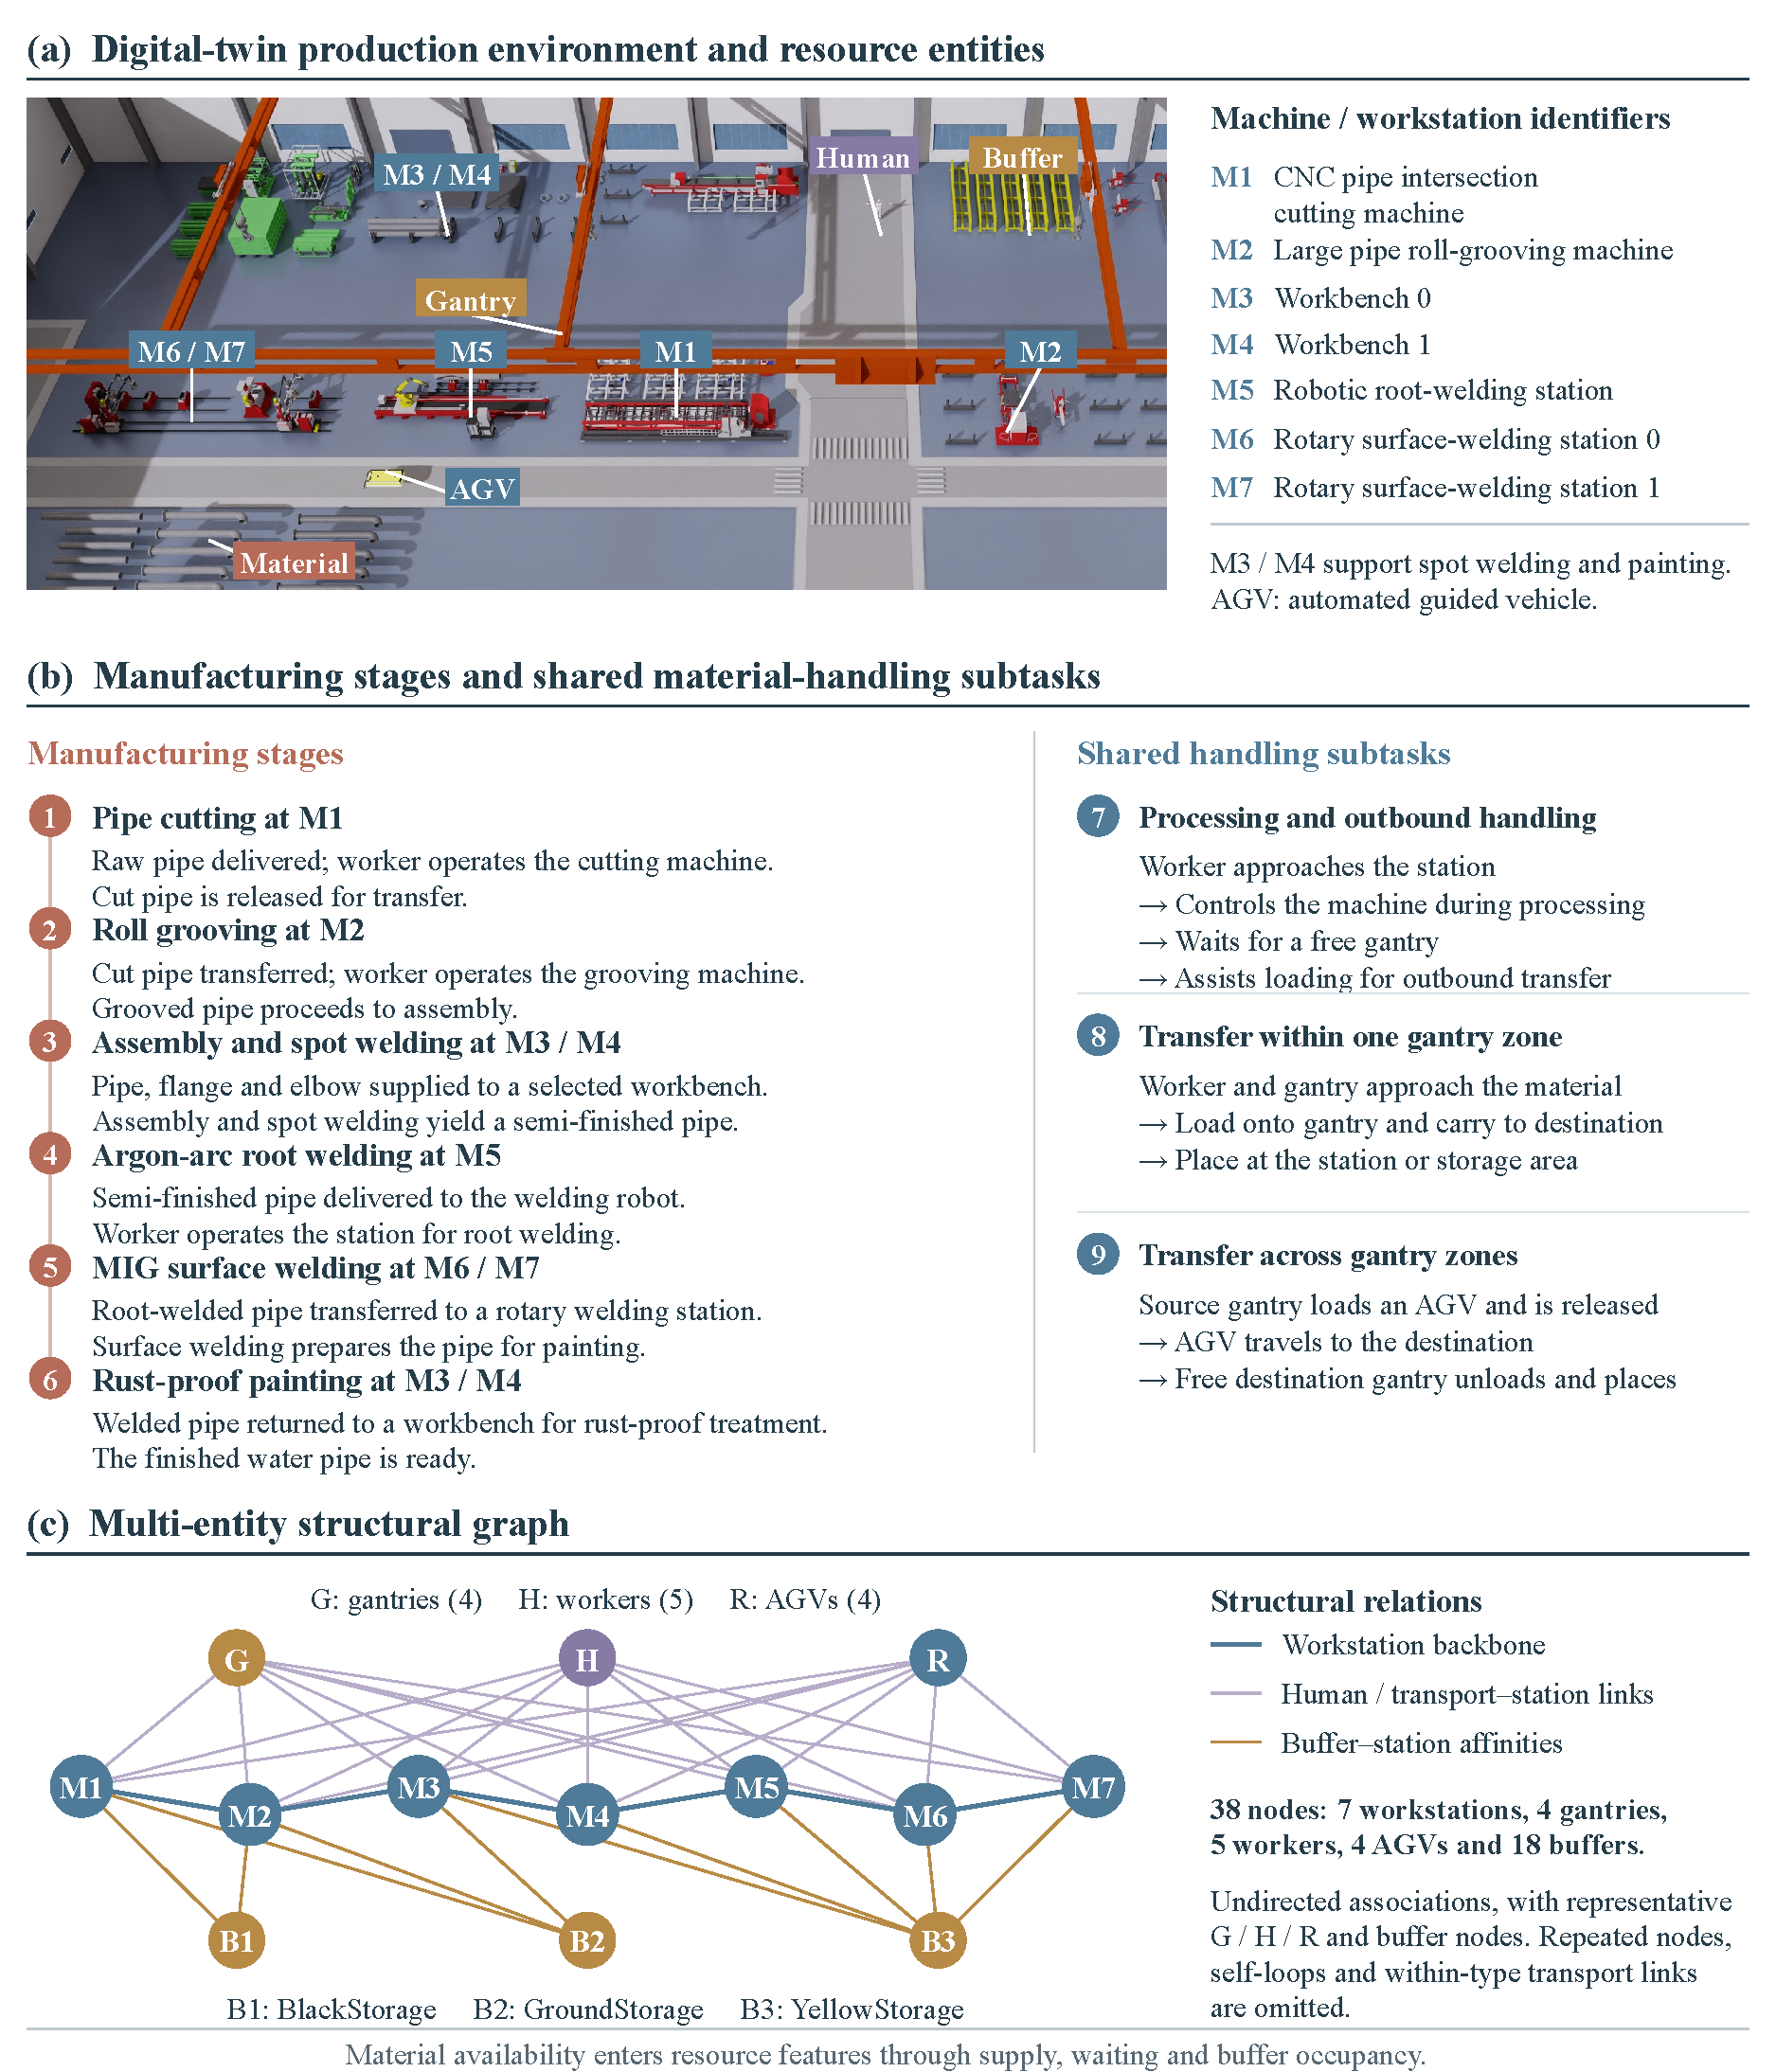
\includegraphics[width=\textwidth]{figures/fig_experiment.pdf}
\caption{Open-workspace factory model developed for NVIDIA Isaac Sim: (a)~resource entities; (b)~manufacturing stages; (c)~structural graph of 38 resources.}
\label{fig:experiment}
\end{figure*}

The data-generation environment exposes four operating variation dimensions and applies each dimension at three intervention levels (Table~\ref{tab:disturbance-design}). Level~0 changes episode-wide resource capacity before each model run, Level~1 perturbs sampled processing or service behaviour, and Level~2 injects temporary events during production. The platform supports intensity $I\in\{1,2,3\}$; slash-separated values in the table follow this order. The formal \texttt{dense\_i1} collection activates one dimension at a time at $I=1$, while nominal runs keep all dimensions inactive. The injected dimension controls data generation but is not used as the bottleneck or process-cause label.

\zhpara{数据生成环境围绕工位、人员、物流和物料四个维度设置扰动，并在配置级、采样级和运行时事件级三个层面实施（表~\ref{tab:disturbance-design}）。L0 在仿真开始前改变整局资源能力，L1 改变加工或服务过程的随机采样，L2 在生产过程中注入有起止时间的临时事件。环境支持 $I\in\{1,2,3\}$ 三档强度，表中斜线分隔值依次对应三档。正式 \texttt{dense\_i1} 数据每次仅激活一个扰动维度且固定 $I=1$，无扰动运行保持全部维度为标称状态；二维、三维和四维混合扰动另行保存，不并入主数据集。这样的设计既保留了注入条件的可追溯性，也避免把扰动维度直接当作瓶颈标签或过程原因标签。}

\begin{table*}[t]
\centering
\caption{Four operating variation dimensions and their three intervention levels. Values separated by slashes correspond to $I=1/2/3$. One model step equals one logical second.}
\label{tab:disturbance-design}
\scriptsize
\setlength{\tabcolsep}{3.2pt}
\renewcommand{\arraystretch}{1.12}
\begin{tabularx}{\FullWidth}{@{}lXXX@{}}
\toprule
Dimension & L0: episode configuration & L1: sampled process variation & L2: temporary runtime events \\
\midrule
workstation & Disable workbench ws1 and rotary-welding ws1 & Processing-time noise $5/10/15$ steps; success rate $0.88/0.76/0.64$; tool wear $15/30/45$ steps per 1,000 steps & $2/(2$--$3)/(3$--$4)$ idle-station failures; additional $1$--$2/2$--$3/3$--$4$ weld or kitting quality-hold windows \\
Worker & Reduce workers from 5 to $3/2/1$ & Service-time scale $1.55/2.10/2.65$; worker-specific skill range $0.8$--$1.4/0.7$--$1.6/0.6$--$1.8$; time noise $12/22/32$ steps & $2/(2$--$3)/(3$--$4)$ temporary absences, applied only when the selected worker is idle \\
Logistics & Reduce AGVs from 4 to $2/1/1$; retain all four zone gantries & Gantry-time scale $1.65/2.30/2.95$ with motion noise $10/18/26$ steps; weak background process variation & $2/(2$--$3)/(3$--$4)$ gantry or AGV freezes; at least one pulse targets an AGV while other vehicles remain active \\
Material & Keep the nominal inventory of ten pipes, flanges, and elbows; no permanent deletion & At steps 400--1,000, temporarily hide $6$--$7/7$--$8/7$--$8$ idle flanges or elbows for $1{,}400$--$2{,}200/2{,}000$--$2{,}700/2{,}500$--$3{,}200$ steps & After the opening shortage, inject $1$--$2/2$--$3/3$--$4$ complementary flange/elbow shortage pulses; pipe blanks are never hidden \\
\bottomrule
\end{tabularx}
\end{table*}

For workstation, worker, and logistics operating variations, every Level~2 pulse lasts at least 600 steps and the intensity-specific upper bounds are 900/1,300/1,400 steps. Event targets, start times, counts, and durations are resampled for each episode using a deterministic seed. Adjacent pulses are separated by at least 360 steps, and an event waits for an eligible idle target rather than interrupting an active operation. These controls make the injected condition long enough to survive the eight-window persistence filter while avoiding a deterministic one-to-one mapping between an injection and a labelled bottleneck.

\zhpara{对于工位、人员和物流扰动，每个 L2 脉冲至少持续六百步，三档强度的时长上限分别为 900/1,300/1,400 步。目标、起点、条数和时长在每个 episode 中依据固定种子重新采样，相邻事件至少间隔三百六十步；若目标资源正在作业，事件等待其空闲后再生效，而不直接打断加工。该约束使扰动能够跨越八窗口持续性过滤，同时避免注入事件与最终瓶颈标签形成确定的一一对应。}

Raw records use logical model time at one-second resolution and include resource-state transitions, workpiece routes and completion times, buffer changes, transport tasks, material inventories, and operating variation logs. The aggregation pipeline reconstructs resource-state intervals and aligns them into non-overlapping 60-s windows. Processing, blockage, starvation, and stoppage durations are accumulated over their overlap with each window; active and unavailable ratios divide the corresponding durations by the window length. Queue features count waiting jobs and summarize their waiting times, while buffer occupancy is averaged over recorded values in the window (carrying forward the preceding value when no update is recorded) and its growth is computed from the difference between the window-end and window-start counts. Process and transport relations supply upstream/downstream state ratios, route delay, inbound waiting, and material-shortage propagation.

\zhpara{原始记录采用分辨率为一秒的逻辑仿真时间，包括资源状态转换、工件路线与完成时间、缓冲区变化、运输任务、物料库存及扰动日志。聚合流程先重建资源状态区间，再将其对齐到互不重叠的六十秒窗口。加工、阻塞、饥饿与停机时长按状态区间与窗口的重叠部分累计，活动率和不可用率由相应时长除以窗口长度得到；队列特征统计等待工件数及其等待时间，缓冲区占用取窗口内记录值的均值，无更新时沿用前值，增长率由窗口起止库存差除以窗口长度得到。工艺与运输关联进一步提供上下游状态比例、路径延迟、入站等待和物料短缺传播信息。}

All windows share a fixed resource ordering. Each node has 21 operational channels, a five-dimensional resource-type encoding, and one labour-saturation channel, forming a $38\times27$ feature matrix per window. The export routine fills absent numeric entries with zero and recomputes labour saturation from worker activity. Each valid episode ends after all ten workpieces have completed. Runs affected by the known model deadlock defect are discarded as invalid records rather than interpreted as observations of a production operating variation. A run-stratified, episode-level split gives 140/28/36 training/validation/test episodes from 204 valid episodes. Sliding samples use 30 historical windows and a 30-window future grid, with a one-window stride and no crossing of episode boundaries. The resulting partitions contain 20,826/4,331/5,354 forecast windows (Table~\ref{tab:exp-dataset}); feature standardization is fitted on the training histories and applied unchanged to validation and test inputs. All main baseline comparisons use a unified re-evaluation on the same 5,354 shared test-window identities rather than scores from an earlier sample set. Table~\ref{tab:dataset-labels} reports the Upcoming, Ongoing, and no-event composition of the test window--resource pairs under each Start cap.

\zhpara{各窗口采用固定的资源顺序。每个节点包含二十一个运行特征、五维资源类型编码和一个人员饱和度特征，构成每窗口 $38\times27$ 的特征矩阵。导出流程将缺失数值填零，并根据人员活动重新计算人员饱和度。每个有效 episode 在十件工件全部完成后结束。受已知模型死锁缺陷影响的运行作为无效模型记录剔除，而不解释为生产运行变化观测。二百零四个有效 episode 按运行组分层、以 episode 为单位划分为 140/28/36 个训练、验证和测试 episode。滑动样本采用三十个历史窗口与三十个未来窗口网格，步长为一个窗口，且不跨越 episode 边界。最终得到 20{,}826/4{,}331/5{,}354 个预测窗口（表~\ref{tab:exp-dataset}）；特征标准化参数由训练历史拟合，并原样应用于验证与测试输入。主要基线比较均在同一批 5{,}354 个共享测试窗口身份上统一重评，而非沿用更早样本集上的分数。表~\ref{tab:dataset-labels}给出各 Start cap 下测试窗口—资源对的 Upcoming、Ongoing 与无事件构成。}

Operational-state rules combine processing activity, queue buildup, starvation, and resource-coupling indicators into resource-level bottleneck labels. Process-cause targets are derived from the corresponding operating evidence; the report uses material shortage, transport delay, queue buildup, and downstream blockage. Workpiece completion records provide the order-level target: the time from the forecast origin until all ten workpieces have finished.

\zhpara{运行状态规则将加工活动、队列积压、饥饿与资源耦合指标综合为资源级瓶颈标签。过程原因目标由相应运行证据导出；报告使用物料短缺、运输延迟、队列积压与下游阻塞。工件完工记录提供订单级目标：从预报起点到十件工件全部完成的时间。}

Process-informed labels apply an eight-window persistence rule (Min8) to newly forming bottlenecks. An event already active at the last historical window is retained when at least one labelled future window remains. We evaluate three onset-cap settings, Start$\leq5$, Start$\leq10$, and Start$\leq15$, which define the admissible distance between the current window and a future event onset. The future grid and the onset cap are kept fixed within each task. A three-window start tolerance is used for strict report matching, and every window corresponds to 60~s; duration, start, and remaining-time errors are consequently reported in minutes.

\zhpara{过程知情标签对新形成瓶颈采用八窗口持续性规则（Min8）；对于最后一个历史窗口已处于活动状态的事件，只要未来仍有至少一个带标签窗口，就保留其剩余部分。实验设置三个事件起点范围：Start$\leq5$、Start$\leq10$ 和 Start$\leq15$，分别规定当前窗口与未来事件开始之间允许的最大距离。每个任务内部固定未来标签网格和起点上限；严格事件报告采用三个窗口的起点容差。每个窗口对应六十秒，因此持续时间、起点和剩余时间误差均以分钟报告。}

\begin{table}[pos=t]
\centering
\caption{Dataset and label protocol used in the experiments.}
\label{tab:exp-dataset}
\scriptsize
\setlength{\tabcolsep}{4pt}
\renewcommand{\arraystretch}{1.08}
\begin{tabularx}{\columnwidth}{@{}lX@{}}
\toprule
Item & Setting \\
\midrule
Dataset & \texttt{dense\_i1}, 204 valid episodes, 38 resources \\
Split & 140/28/36 episodes; 20,826/4,331/5,354 windows \\
Windowing & 60-s windows; 30 historical + 30 future windows \\
Targets & 15 resources: 7 workstations, 4 gantries, 4 robots \\
Event rule & Min8 persistence; Start$\leq5/10/15$ \\
Report matching & Three-window onset tolerance \\
\bottomrule
\end{tabularx}
\end{table}

\begin{table}[pos=t]
\centering
\caption{Test-set label composition under each Start cap. Counts are window--resource pairs over 5,354 windows $\times$ 15 targets ($80{,}310$ pairs); parentheses give the share of all pairs.}
\label{tab:dataset-labels}
\scriptsize
\setlength{\tabcolsep}{3.2pt}
\renewcommand{\arraystretch}{1.08}
\begin{tabular*}{\columnwidth}{@{\extracolsep{\fill}}lrrr@{}}
\toprule
Start cap & Upcoming & Ongoing & No-event \\
\midrule
$\leq5$ & 336 (0.42\%) & 766 (0.95\%) & 79,208 (98.63\%) \\
$\leq10$ & 604 (0.75\%) & 768 (0.96\%) & 78,938 (98.29\%) \\
$\leq15$ & 708 (0.88\%) & 770 (0.96\%) & 78,832 (98.16\%) \\
\bottomrule
\end{tabular*}
\end{table}

\subsubsection{Baseline methods}

Four baselines represent complementary modelling families. XGBoost is a gradient-boosted decision-tree predictor operating on tabular summaries, providing a non-neural reference for nonlinear feature interactions. LSTM is a recurrent predictor that models temporal dependencies in the historical sequence. BTGCN constructs a graph over production tasks and combines graph convolution with a GRU to model relational and temporal information~\cite{yin2025btgcn}. BSTAN uses graph attention with a GRU to learn adaptive neighbour contributions for blockage and starvation related prediction~\cite{lai2023bstan}. All baseline comparisons reported in this paper use a unified re-evaluation on the same 5,354 shared test windows, with identical sample identities, history length, future grid, target resources, and event-label definitions for PHGST-DM and the four baselines. Each baseline retains its corresponding input representation and training procedure.

\zhpara{匹配比较包含四种模型族。XGBoost 是作用于表格统计量的梯度提升决策树模型，为非神经模型提供非线性交互参考；LSTM 是利用循环结构建模历史序列时间依赖的预测器；BTGCN 在生产任务之间构造图，并结合图卷积与 GRU 建模关系和时间信息~\cite{yin2025btgcn}；BSTAN 使用图注意力和 GRU 学习邻居资源的自适应贡献，用于与阻塞和饥饿相关的预测~\cite{lai2023bstan}。统一比较为五种模型规定相同的历史长度、未来标签网格、目标资源和事件标签定义，各基线采用其对应的输入表示与训练流程。}

\begin{table}[pos=t]
\centering
\caption{Baseline models and their roles in the comparison.}
\label{tab:exp-baselines}
\scriptsize
\setlength{\tabcolsep}{4pt}
\renewcommand{\arraystretch}{1.10}
\begin{tabularx}{\columnwidth}{@{}lXX@{}}
\toprule
Model & Core framework & Comparison role \\
\midrule
XGBoost & Gradient-boosted decision trees & Tabular predictor \\
LSTM & Long short-term memory & Recurrent temporal predictor \\
BTGCN & Graph convolution + GRU & Graph-convolutional predictor \\
BSTAN & Graph attention + GRU & Graph-attention predictor \\
\bottomrule
\end{tabularx}
\end{table}

\subsubsection{Overall experimental settings and metrics}

PHGST-DM uses five encoder blocks, an 80-dimensional latent representation, eight-dimensional Laplacian positional encoding, $4/2/2$ temporal/geographic/semantic attention heads, a geographic hop-distance cutoff of 4, five semantic neighbours, and 16 length-three pattern keys. AdamW is used with batch size 16, learning rate $5\times10^{-5}$, weight decay $0.05$, cosine decay to $10^{-6}$, and fourfold positive-window oversampling. Training has two stages. Stage~1 learns the bottleneck and cause heads: it starts from the fixed parameter state reused by every ablation arm, unfreezes the last five encoder blocks, and runs for at most 50 epochs with patience 40. The three onset caps are trained as a curriculum (Start$\leq5\rightarrow$Start$\leq10\rightarrow$Start$\leq15$). A far-onset enhancement doubles the onset loss for events starting more than 5~min ahead, sets the far-onset positive weight to $9/10/11$ for the three caps, and raises the false-alarm penalty (weights $2.5$ and $2.2$ for ordinary and hard false positives). Stage~2 freezes the encoder and every bottleneck and cause head, adds a per-workpiece rate term to the remaining-time head, and fine-tunes only that head for at most 20 epochs with validation loss as the selection criterion. This stage specializes the order-progress forecast while preserving the event and cause outputs. All reported training runs use seed 42; the results are point estimates rather than multi-seed stability estimates. Table~\ref{tab:shared-training-protocol} summarizes the shared training and model settings; Appendix~\ref{app:additional} gives the loss weights, label thresholds, and decoding details.

\zhpara{PHGST-DM 使用五个编码器模块、八十维潜表示、八维拉普拉斯位置编码、$4/2/2$ 的时间/地理/语义注意力头、地理跳数截断为 4、五个语义邻居和十六个长度为三的模式键。训练使用 AdamW，batch size 为 16，学习率为 $5\times10^{-5}$，权重衰减为 $0.05$，余弦衰减下限为 $10^{-6}$，并对正例窗口进行四倍过采样。训练分为两个阶段。第一阶段学习瓶颈头和原因头：从各消融分支共用的固定参数状态起步，解冻编码器最后五个模块，最多训练 50 个 epoch，patience 为 40。三个起点范围按课程依次训练（Start$\leq5\rightarrow$Start$\leq10\rightarrow$Start$\leq15$）。远期增强将起点超过五分钟的事件的起点损失加倍，三个范围的远期正样本权重分别设为 $9/10/11$，并提高误报惩罚（普通与困难误报权重分别为 $2.5$ 与 $2.2$）。第二阶段冻结编码器以及全部瓶颈头和原因头，为剩余时间头增加按工件计的速率项，仅微调该头，最多二十个 epoch，并以验证损失选模。该阶段专项优化订单进度预测，同时保持事件与原因输出。所有报告训练均使用 seed 42；结果为点估计，而非多种子稳定性估计。表~\ref{tab:shared-training-protocol}与表~\ref{tab:model-task-parameters}汇总所报告 Full 与消融比较采用的完整共用协议与模型设置。}

The checkpoint and report threshold are selected on the validation split. Candidate thresholds are $\{0.45,\dots,0.90,0.94\}$; selection uses the internal station-identification F1 among candidates satisfying validation report precision $\geq0.80$ and recall $\geq0.70$. This selection score is not reported as a result; the reported event metric is the onset-qualified F1-score defined below. All three onset caps use the selected threshold of $0.94$ for testing.

\zhpara{checkpoint 与报告阈值依据验证集选择。候选阈值为 $\{0.45,\dots,0.90,0.94\}$；在满足验证报告精确率 $\geq0.80$、召回率 $\geq0.70$ 的候选中，使用内部工位识别 F1 选择工作点。该选择分数不作为结果报告；正式事件指标采用下文定义的、包含起点容差的 F1-score。三个起点范围的测试均采用选定阈值 $0.94$。}

Metrics follow the three prediction dimensions. The reported bottleneck-event F1-score requires both correct station identification and an onset error within three windows. Upcoming recall uses future-event window--resource pairs whose final historical window is non-bottleneck; Ongoing recall uses pairs with an active final historical window. Start and duration MAE are measured on correctly detected events, while union duration MAE/RMSE includes missed and false events. Next-window and 30-window State F1 describe the predicted occupancy over time, including recovery. Process-cause evaluation uses accuracy and macro recall over the four supported classes. Order-completion evaluation uses remaining-time MAE at the line level.

\zhpara{评价指标围绕三个预测维度组织。正式报告的瓶颈事件 F1-score 同时要求工位识别正确且起点误差不超过三个窗口。Upcoming 召回率在最后历史窗口尚未处于瓶颈的未来事件窗口—资源对上计算，Ongoing 召回率对应历史末端已有活动瓶颈的样本。起点与持续时间 MAE 在正确识别的事件上计算，union 持续时间 MAE/RMSE 同时计入漏报与误报；下一窗口与三十窗口 State F1 描述随时间变化的占用状态，包括恢复过程。过程原因评价采用四个有支持类别上的准确率与宏平均召回率，订单完成评价采用产线级剩余时间 MAE。}

\begin{table*}[t]
\centering
\caption{Metrics used in the main evaluation and component analyses.}
\label{tab:exp-metrics}
\scriptsize
\setlength{\tabcolsep}{3.5pt}
\renewcommand{\arraystretch}{1.08}
\begin{tabular*}{\FullWidth}{@{\extracolsep{\fill}}lll@{}}
\toprule
Metric group & Metric & Interpretation \\
\midrule
Event & F1-score & Station identification with a three-window onset tolerance \\
Early warning & Upcoming / ongoing recall & Station recall: historically cold / active resources \\
State & State F1 (1-step / horizon) & Bottleneck state accuracy at one step / 30-step horizon \\
Temporal & Start MAE; duration MAE & Localization and duration error on detected events \\
Temporal & Union duration MAE/RMSE & Error including missed and false events \\
Auxiliary & Remaining-time MAE & Global order-progress estimation error \\
Auxiliary & Cause accuracy / macro recall & Four supported process-cause classes \\
\bottomrule
\end{tabular*}
\end{table*}

\subsection{Main and baseline performance comparison}\label{sec:comparison-overview}

The comparison evaluates three complementary capabilities of the production forecast. Bottleneck event and temporal prediction identifies the affected resource and describes when its constraint begins, persists, and ends (Table~\ref{tab:comparison-main}); process-cause prediction supplies an operational interpretation of that constraint (Table~\ref{tab:comparison-state}); and order remaining-time prediction estimates line-level completion progress (Table~\ref{tab:comparison-remain}). Together, these outputs provide resource-level warning with process context and an order-progress estimate. All baseline comparisons in this section use a unified re-evaluation on the same 5,354 shared test windows (and the corresponding window--resource pairs), with identical sample identities, target resources, future grid, and label definitions for PHGST-DM and the four baselines.

\zhpara{该比较从生产预报的三项互补能力展开。瓶颈事件与时间预测识别受影响资源，并描述约束何时开始、持续与结束（表~\ref{tab:comparison-main}）；过程原因预测为该约束提供运行解释（表~\ref{tab:comparison-state}）；订单剩余时间预测估计产线级完工进度（表~\ref{tab:comparison-remain}）。三者共同构成带有过程上下文的资源级预警与订单进度估计。本节报告的全部基线比较均在同一批 5{,}354 个共享测试窗口（及对应窗口—资源对）上统一重评，PHGST-DM 与四个基线使用相同的样本身份、目标资源、未来网格与标签定义。}

\subsubsection{Bottleneck occurrence, onset, end, and duration}\label{sec:comparison-event}

PHGST-DM couples resource identification with the expected bottleneck interval and its evolving occupancy. Table~\ref{tab:comparison-main} evaluates this capability through event P/R/F1, Upcoming/Ongoing recall, onset and duration MAE, and one-step/30-step State F1. Onset and duration jointly specify the reported interval within the 30-min horizon, while the future state sequence describes persistence and recovery. Temporal MAE is evaluated on correctly detected events and is read alongside event recall to characterize both coverage and localization.

\zhpara{PHGST-DM 将资源识别、瓶颈时间区间及其占用变化联合起来。表~\ref{tab:comparison-main}通过事件 P/R/F1、Upcoming/Ongoing 召回率、起点与持续时间 MAE，以及单步和三十步 State F1 评价这一能力。起点与持续时间共同描述三十分钟预测范围内的报告区间，未来状态序列进一步刻画持续与恢复过程。时间 MAE 在正确检出的事件上评价，并与事件召回率共同反映覆盖范围和时间定位表现。}

PHGST-DM combines broad event coverage with early warning across the three onset caps. F1-score reaches $0.804/0.778/0.768$; the reported differences from the strongest baseline are $10.2/16.7/19.1$ percentage points. Upcoming recall remains $0.542/0.535/0.537$, alongside Ongoing recall of $0.937/0.939/0.930$. These results indicate that PHGST-DM detects upcoming bottlenecks while maintaining coverage of ongoing events.

\zhpara{PHGST-DM 在三个起点范围下同时保持较广的事件覆盖与提前预警。F1-score 达到 $0.804/0.778/0.768$，相对最强基线的报告差值为 $10.2/16.7/19.1$ 个百分点。Upcoming 召回率保持为 $0.542/0.535/0.537$，Ongoing 召回率为 $0.937/0.939/0.930$。结果表明，PHGST-DM 在识别即将发生的瓶颈的同时，仍保持对进行中事件的覆盖。}

\begin{table*}[t]
\centering
\caption{Bottleneck event and temporal prediction. Classification scores are percentages; timing MAE is in minutes. Within each Start cap, bold marks the best value and underline marks second-best. All entries use the unified 5,354-window re-evaluation in Section~\ref{sec:comparison-overview}.}
\label{tab:comparison-main}
\scriptsize
\setlength{\tabcolsep}{3.2pt}
\renewcommand{\arraystretch}{1.12}
\begin{tabular*}{\FullWidth}{@{\extracolsep{\fill}}lrrrrrrr@{}}
\toprule
Model & \multicolumn{1}{c}{Event identification $\uparrow$} & \multicolumn{2}{c}{Event recall $\uparrow$} & \multicolumn{2}{c}{Timing MAE $\downarrow$} & \multicolumn{2}{c}{State F1 $\uparrow$} \\
\cmidrule(lr){2-2}\cmidrule(lr){3-4}\cmidrule(lr){5-6}\cmidrule(l){7-8}
 & F1-score & Upcoming & Ongoing & Start & Duration & 1 step & 30 steps \\
\midrule
\multicolumn{8}{l}{\textit{Start $\leq5$}} \\
PHGST-DM & \textbf{80.4\%} & \textbf{54.2\%} & \textbf{93.7\%} & 0.127 & \textbf{1.863} & \textbf{88.3\%} & \textbf{52.5\%} \\
XGBoost & \underline{70.2\%} & 6.0\% & \underline{81.9\%} & \underline{0.030} & \underline{3.264} & 61.1\% & 37.3\% \\
LSTM & 58.3\% & \underline{9.9\%} & 68.7\% & 0.056 & 3.855 & 29.5\% & 29.5\% \\
BTGCN & 66.9\% & 4.6\% & 78.6\% & \textbf{0.020} & 3.322 & 64.3\% & 37.2\% \\
BSTAN & 68.7\% & 9.5\% & 79.4\% & 0.043 & 3.565 & \underline{71.9\%} & \underline{37.9\%} \\
\midrule
\multicolumn{8}{l}{\textit{Start $\leq10$}} \\
PHGST-DM & \textbf{77.8\%} & \textbf{53.5\%} & \textbf{93.9\%} & 0.227 & \textbf{1.788} & \textbf{89.2\%} & \textbf{58.9\%} \\
XGBoost & \underline{61.1\%} & 4.1\% & \underline{80.5\%} & \underline{0.122} & \underline{3.210} & 59.5\% & 33.7\% \\
LSTM & 47.7\% & \underline{11.2\%} & 69.3\% & 0.388 & 3.768 & 27.5\% & 26.2\% \\
BTGCN & 57.9\% & 4.5\% & 72.2\% & \textbf{0.117} & 3.238 & 56.6\% & 35.9\% \\
BSTAN & 60.9\% & 5.7\% & 79.6\% & 0.153 & 3.533 & \underline{63.2\%} & \underline{36.5\%} \\
\midrule
\multicolumn{8}{l}{\textit{Start $\leq15$}} \\
PHGST-DM & \textbf{76.8\%} & \textbf{53.7\%} & \textbf{93.0\%} & 0.227 & \textbf{1.716} & \textbf{90.0\%} & \textbf{61.0\%} \\
XGBoost & \underline{57.7\%} & 3.9\% & \underline{79.6\%} & \textbf{0.167} & 3.170 & 58.2\% & 32.2\% \\
LSTM & 46.1\% & \underline{10.2\%} & 64.3\% & 0.453 & 3.615 & 26.8\% & 26.0\% \\
BTGCN & 51.8\% & 5.4\% & 69.9\% & 0.302 & \underline{3.121} & 46.1\% & 32.3\% \\
BSTAN & 53.4\% & 4.4\% & 70.0\% & \underline{0.222} & 3.422 & \underline{59.3\%} & \underline{33.5\%} \\
\bottomrule
\end{tabular*}
\end{table*}

The temporal outputs extend event identification into a forecast of how long a resource will remain constrained. PHGST-DM's onset MAE is $0.127/0.227/0.227$~min, and detected-event duration MAE is $1.863/1.788/1.716$~min. The latter corresponds to reductions of $42.9\%/44.3\%/45.0\%$ relative to the lowest reported baseline errors. One-step State F1 reaches $0.883/0.892/0.900$, and 30-step State F1 reaches $0.525/0.589/0.610$, exceeding the strongest reported baseline by $14.6/22.4/27.5$ percentage points at the full horizon. Together, the onset, duration, and occupancy predictions describe when a resource is expected to become constrained and recover, providing temporal context for intervention planning. Figure~\ref{fig:baseline-comparison} summarizes F1-score, Upcoming recall, and duration MAE: PHGST-DM maintains Upcoming recall near $0.54$ and duration MAE below 2~min across all three cap settings.

\zhpara{时间输出将事件识别进一步扩展为资源持续受限过程的预测。PHGST-DM 的起点 MAE 为 $0.127/0.227/0.227$ 分钟，正确检出事件的持续时间 MAE 为 $1.863/1.788/1.716$ 分钟，后者相对于已报告误差最低的基线下降 $42.9\%/44.3\%/45.0\%$。单步 State F1 达到 $0.883/0.892/0.900$，三十步 State F1 达到 $0.525/0.589/0.610$；在完整预测范围内，后者高于已报告最佳基线 $14.6/22.4/27.5$ 个百分点。起点定位、持续时间估计和占用预测共同描述了可用于规划资源关注与恢复的时间区间。图~\ref{fig:baseline-comparison}汇总 F1-score、Upcoming 召回率和持续时间 MAE：PHGST-DM 在三个起点范围下的 Upcoming 召回率均保持在 $0.54$ 左右，持续时间 MAE 均低于两分钟。}

\begin{figure*}[t]
\centering
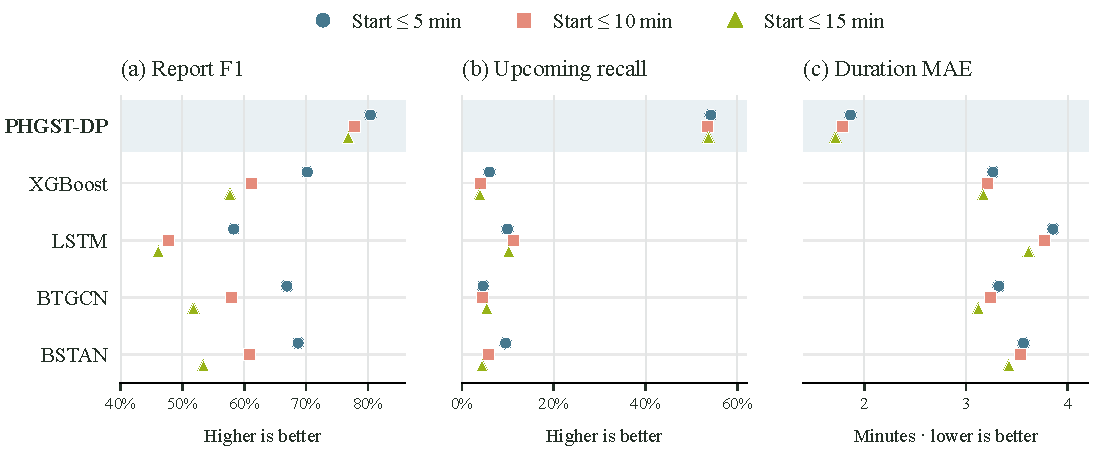
\includegraphics[width=0.96\textwidth]{figures/fig_range_response.pdf}
\caption{Grouped comparison of (a)~F1-score, (b)~Upcoming recall, and (c)~detected-event duration MAE across Start caps.}
\label{fig:baseline-comparison}
\end{figure*}

Within the Start$\leq15$ task, grouping events by their true onset distance shows how warning extends into the future: strict report recall is $0.574$, $0.522$, and $0.433$ for onsets within 5, 6--10, and more than 10~min, respectively. The last group directly demonstrates warning coverage beyond 10~min. Across the three separately configured cap tasks, exact-onset accuracy among station-matched true positives is $0.896/0.844/0.831$, and onset-bucket accuracy is $0.921/0.918/0.920$. Warning also spans processing and material handling: workstation/gantry/robot F1 is $0.805/0.811/0.771$ at Start$\leq5$ and $0.751/0.840/0.639$ at Start$\leq15$. These results place the temporal forecast across the resource types through which production constraints emerge.

\zhpara{在 Start$\leq15$ 任务内部，按真实起点距离分组可以展示预警向未来延伸的覆盖情况：五分钟内、六至十分钟及十分钟以后事件的严格报告召回率分别为 $0.574$、$0.522$ 和 $0.433$，其中最后一组直接体现十分钟以后的预警覆盖。在三个分别配置的起点范围任务中，工位匹配成功的真阳性样本的精确起点准确率为 $0.896/0.844/0.831$，起点分档准确率为 $0.921/0.918/0.920$。预警还覆盖加工与物料搬运资源：机器/龙门/运输机器人的 F1 在 Start$\leq5$ 下为 $0.805/0.811/0.771$，在 Start$\leq15$ 下为 $0.751/0.840/0.639$。这些结果将时间预测扩展到生产约束形成过程中涉及的多类资源。}

\subsubsection{Bottleneck process-cause prediction}\label{sec:comparison-cause}

PHGST-DM predicts process causes alongside its event and temporal forecasts, with cause accuracy of $0.965/0.962/0.974$ and macro recall of $0.967/0.965/0.978$ across the three caps (Table~\ref{tab:comparison-state}). XGBoost records the highest values, with accuracy of $0.990$ and macro recall of $0.988$ under each cap. PHGST-DM ranks second, trailing XGBoost by $1.6$--$2.8$ percentage points in accuracy and $1.0$--$2.3$ points in macro recall. It outperforms the three neural baselines on both metrics under every cap. Its cause classification output complements event coverage by providing graph-level process context in the categories of material shortage, transport delay, queue buildup, and downstream blockage.

\zhpara{PHGST-DM 在事件与时间预测之外同时给出过程解释：三个 cap 下原因准确率为 $0.965/0.962/0.974$，宏平均召回率为 $0.967/0.965/0.978$（表~\ref{tab:comparison-state}）。XGBoost 取得最高值，各 cap 下准确率均为 $0.990$、宏平均召回率均为 $0.988$。PHGST-DM 位列第二，准确率仅落后 XGBoost $1.6$--$2.8$ 个百分点，宏平均召回率落后 $1.0$--$2.3$ 个百分点，并在每个 cap 的两项指标上均优于三个神经基线。其具有竞争力的原因识别与事件覆盖相互补充，可将所预测的资源与时间区间关联到物料短缺、运输延迟、队列积压或下游阻塞。}

\begin{table*}[t]
\centering
\caption{Bottleneck process-cause prediction (\%). Each Start-cap group reports accuracy and macro recall. Within each Start-cap metric, bold marks the best value and underline marks second-best among the compared models. All entries use the unified 5,354-window re-evaluation in Section~\ref{sec:comparison-overview}.}
\label{tab:comparison-state}
\scriptsize
\setlength{\tabcolsep}{3.2pt}
\renewcommand{\arraystretch}{1.12}
\begin{tabular*}{\FullWidth}{@{\extracolsep{\fill}}lrrrrrr@{}}
\toprule
Model & \multicolumn{2}{c}{Start $\leq5$} & \multicolumn{2}{c}{Start $\leq10$} & \multicolumn{2}{c}{Start $\leq15$} \\
\cmidrule(lr){2-3}\cmidrule(lr){4-5}\cmidrule(l){6-7}
 & Accuracy $\uparrow$ & Macro R $\uparrow$ & Accuracy $\uparrow$ & Macro R $\uparrow$ & Accuracy $\uparrow$ & Macro R $\uparrow$ \\
\midrule
PHGST-DM & \underline{96.5\%} & \underline{96.7\%} & \underline{96.2\%} & \underline{96.5\%} & \underline{97.4\%} & \underline{97.8\%} \\
XGBoost & \textbf{99.0\%} & \textbf{98.8\%} & \textbf{99.0\%} & \textbf{98.8\%} & \textbf{99.0\%} & \textbf{98.8\%} \\
LSTM & 93.8\% & 92.0\% & 93.6\% & 93.0\% & 94.4\% & 92.2\% \\
BTGCN & 90.0\% & 88.2\% & 90.7\% & 90.0\% & 90.7\% & 90.0\% \\
BSTAN & 95.7\% & 95.2\% & 95.9\% & 95.1\% & 95.1\% & 93.5\% \\
\bottomrule
\end{tabular*}
\end{table*}


\subsubsection{Order-completion remaining-time prediction}\label{sec:comparison-remain}

Order remaining time is a line-level scalar target that complements resource-level bottleneck forecasts. Table~\ref{tab:comparison-remain} reports global remaining-time MAE under the same unified 5,354-window re-evaluation used for the event and cause comparisons. XGBoost records the lowest MAE, $5.23$~min under each Start cap, whereas PHGST-DM after stage-2 fine-tuning records $9.60/9.27/8.91$~min at Start$\leq5/10/15$. Under this common-sample protocol, XGBoost is the more accurate order remaining-time predictor among the compared models.

\zhpara{订单剩余时间是对资源级瓶颈预报的产线级标量补充。表~\ref{tab:comparison-remain}在与事件、原因比较相同的统一 5{,}354 窗口重评协议下报告全局剩余时间 MAE。XGBoost 的 MAE 最低，各 Start cap 下均为 $5.23$~min；经第 2 阶段微调后的 PHGST-DM 在 Start$\leq5/10/15$ 下为 $9.60/9.27/8.91$~min。在该同一样本协议下，XGBoost 是所比较模型中更准确的订单剩余时间预测器。}

\begin{table}[pos=htbp]
\centering
\caption{Global order remaining-time MAE (min; lower is better). Within each Start cap, bold marks the best value and underline marks second-best. All entries use the unified 5,354-window re-evaluation in Section~\ref{sec:comparison-overview}.}
\label{tab:comparison-remain}
\scriptsize
\setlength{\tabcolsep}{3pt}
\renewcommand{\arraystretch}{1.10}
\begin{tabular*}{\columnwidth}{@{\extracolsep{\fill}}lrrr@{}}
\toprule
Model & Start $\leq5$ & Start $\leq10$ & Start $\leq15$ \\
\midrule
XGBoost & \textbf{5.23} & \textbf{5.23} & \textbf{5.23} \\
LSTM & 10.59 & 10.61 & 9.01 \\
BTGCN & 19.34 & 18.10 & 12.83 \\
BSTAN & 14.70 & 13.85 & 13.56 \\
\midrule
PHGST-DM (stage 1) & 10.93 & 11.21 & 9.72 \\
PHGST-DM (stage 2) & \underline{9.60} & \underline{9.27} & \underline{8.91} \\
\bottomrule
\end{tabular*}
\end{table}

A possible explanation concerns the representation and optimization used for this target. In the baseline design, XGBoost trains an independent remaining-time regressor using recent historical statistics, global state, and explicit order-progress features, including remaining workpiece count, total count, and remaining fraction. Its piecewise nonlinear regression may be well suited to progress--completion-time relationships. PHGST-DM first learns a shared representation for bottleneck events and their temporal and process context; stage~2 freezes the encoder and event and cause heads while optimizing the remaining-time head. PHGST-DM also conditions this head on the remaining workpiece fraction and total count, and its stage-2 rate term uses the remaining count. Thus, the observed gap cannot be attributed simply to an absence of progress information in PHGST-DM. The common-sample results are consistent with the interpretation that independently optimized tree regression fits this order-level target better than the frozen shared representation under the evaluated configuration.

\zhpara{一种可能的解释与该目标所用的表示与优化有关。在基线设计中，XGBoost 使用近期历史统计、全局状态以及显式订单进度特征（包括剩余工件数、总数与剩余比例）训练独立的剩余时间回归器；其分段非线性回归可能较适合进度—完工时间关系。PHGST-DM 首先为瓶颈事件及其时间与过程上下文学习共享表示；第 2 阶段冻结编码器以及事件与原因头，仅优化剩余时间头。PHGST-DM 也以剩余工件比例与总数条件化该头，且其第 2 阶段速率项使用剩余件数。因此，观测到的差距不能简单归因于 PHGST-DM 缺少进度信息。同一样本结果与如下解释一致：在所评估配置下，独立优化的树回归比冻结共享表示更贴合这一订单级目标。}

Stage-2 fine-tuning reduces PHGST-DM MAE from $10.93/11.21/9.72$ to $9.60/9.27/8.91$~min while retaining the event and cause outputs (Figure~\ref{fig:remain-finetune}). This improvement supports the value of task-specific optimization, but does not establish superiority over a dedicated regressor. PHGST-DM's contribution is to report order progress together with resource-level advance warning and process explanations.

\zhpara{第 2 阶段微调将 PHGST-DM 的 MAE 从 $10.93/11.21/9.72$ 降至 $9.60/9.27/8.91$~min，同时保留事件与原因输出（图~\ref{fig:remain-finetune}）。这一改进支持任务特定优化的价值，但并不确立相对专用回归器的优势。PHGST-DM 的贡献在于把订单进度与资源级提前预警及过程解释一并报告。}

\subsection{Ablation study}

The ablation study links predictive performance to three design choices: heterogeneous process--logistics information, process-informed supervision and temporal pattern clustering, and delay-aware modeling. Nine configurations also examine the decoder and training choices that support advance warning (Table~\ref{tab:ablation-arms}). Every ablation comparison, including its Full reference, is evaluated on the same 5,354 shared test windows used in Section~\ref{sec:comparison-overview}, begins from identical parameter values, and uses a 50-epoch budget, the same Start$\leq5\rightarrow$Start$\leq10\rightarrow$Start$\leq15$ curriculum, and the same validation-controlled checkpoint and threshold-selection rule. Dataset, target resources, label rules, and candidate thresholds also follow the same protocol. The common selection procedure yields a threshold of $0.94$ for most arms and $0.90/0.88/0.94$ for NoFarBoost. The matched-budget cause-supervision experiment separately isolates the explanatory effect of the cause head. Remaining-time comparisons within the ablation study use the stage-1 reference, before head-specific fine-tuning.

\zhpara{消融实验将预测性能与三项设计选择联系起来：异构工艺—物流信息、过程知情监督与时间模式聚类，以及延迟感知建模。另有九种配置考察支撑提前预警的解码器与训练选择（表~\ref{tab:ablation-arms}）。每一项消融比较（含 Full 对照）均在第~\ref{sec:comparison-overview}节所用同一批 5{,}354 个共享测试窗口上评估，从相同参数初始化出发，采用 50 个 epoch 预算、相同的 Start$\leq5\rightarrow$Start$\leq10\rightarrow$Start$\leq15$ 课程，以及相同的验证控制检查点与阈值选择规则。数据集、目标资源、标签规则与候选阈值亦遵循同一协议。该共用选择流程对多数分支给出阈值 $0.94$，对 NoFarBoost 给出 $0.90/0.88/0.94$。匹配预算的原因监督实验单独隔离原因头的解释作用。消融内的剩余时间比较使用阶段 1 参考结果，即在头级微调之前。}

\begin{table*}[t]
\centering
\caption{Ablation arms. Every comparison, including the Full reference, begins from identical parameter values and uses the same 50-epoch budget, Start$\leq5\rightarrow$Start$\leq10\rightarrow$Start$\leq15$ curriculum, and validation-controlled model-selection rule.}
\label{tab:ablation-arms}
\scriptsize
\setlength{\tabcolsep}{3.5pt}
\renewcommand{\arraystretch}{1.08}
\begin{tabular*}{\FullWidth}{@{\extracolsep{\fill}}llll@{}}
\toprule
Arm & Contribution & Change relative to the retained model & Training \\
\midrule
NoGraph & Heterogeneous graph & Self-loop adjacency only; no factory edges & Common protocol, 50 ep. \\
NoGroup & Heterogeneous graph & One linear projection of the 27 channels instead of six semantic groups & Common protocol, 50 ep. \\
NoCross & Heterogeneous graph & Within-type edges only; cross-type semantic attention masked & Common protocol, 50 ep. \\
NoInfo & Heterogeneous graph & Only workstations observed; non-workstation features and five coupling channels zeroed & Common protocol, 50 ep. \\
WorkstationOnly & Heterogeneous graph & NoCross and NoInfo combined & Common protocol, 50 ep. \\
NoCluster & Temporal pattern clustering & Temporal pattern clustering removed & Common protocol, 50 ep. \\
NoPattern & \makecell[l]{Delay-aware modeling} & Recent-patch matching to the temporal-pattern prototype bank disabled & Common protocol, 50 ep. \\
NoSplit & Decoder & One shared will head for continuing and new events & Common protocol, 50 ep. \\
NoFarBoost & Training & Far-onset weighting and enhanced false-alarm penalty removed & Common protocol, 50 ep. \\
\bottomrule
\end{tabular*}
\end{table*}

PHGST-DM preserves event accuracy as the onset range expands (Tables~\ref{tab:entity-ablation-new}, \ref{tab:group-ablation}, \ref{tab:delay-ablation-new}, and~\ref{tab:decoder-ablation}). Most removed components lower F1-score and Upcoming recall and raise union duration error, while NoFarBoost is slightly better at Start$\leq5$ at its validation-selected threshold. From Start$\leq5$ to Start$\leq15$, Full F1-score changes from $0.804$ to $0.768$, and union duration MAE from $4.17$ to $4.43$~min. Under the matched initialization, budget, curriculum, and model-selection protocol, the structural and entity variants exhibit larger changes, with F1 reductions of approximately $0.052$--$0.328$ and union duration MAE increases of $0.95$--$3.23$~min across NoGraph, NoGroup, NoCross, NoInfo, and WorkstationOnly over the three onset caps. For delay-aware modeling, Upcoming recall holds with Full across caps, whereas NoPattern and NoSplit degrade more sharply, and the $>10$~min strict-report bin rises from $0.240$ (NoFarBoost) to $0.433$ (Full).

\zhpara{PHGST-DM 在扩大事件起点范围时保持了事件识别精度（表~\ref{tab:ablation-grouped}）。去掉大多数组件后，F1-score 与 Upcoming 召回率下降、union 持续时间误差上升；NoFarBoost 在其自身阈值下于 Start$\leq5$ 略优于 Full。从 Start$\leq5$ 到 Start$\leq15$，Full 的 F1-score 从 $0.804$ 变为 $0.768$，union 持续时间 MAE 从 $4.17$ 分钟变为 $4.43$ 分钟。结构与实体变体在各自训练配置下的变化幅度更大，F1 下降 $0.08$--$0.16$，MAE 上升 $0.8$--$1.5$ 分钟。就延迟模式而言，Full 的 Upcoming 召回率随范围保持稳定，NoPattern 与 NoSplit 退化更明显，且 $>10$ 分钟严格报告召回率由 NoFarBoost 的 $0.240$ 提高到 Full 的 $0.433$。}

\subsubsection{Heterogeneous graph and multi-entity information}

This experiment examines the value of observing multiple resource entities and exchanging information across their process relations (Table~\ref{tab:entity-ablation-new}). NoGraph and NoGroup remove the factory graph and grouped embedding, respectively. NoCross retains all observations and restricts interaction to the same resource type. NoInfo uses workstation observations with five coupling channels masked: route delay, inbound waiting, shortage propagation, blocked-minus-starved time, and labour saturation. WorkstationOnly combines the NoCross and NoInfo restrictions.

\zhpara{本实验考察异构资源观测及跨资源过程信息交换的价值（表~\ref{tab:entity-ablation-new}）。NoGraph 与 NoGroup 分别移除工厂图和分组嵌入；NoCross 保留全部观测，将交互限定在相同资源类型内；NoInfo 使用机器观测，并屏蔽物流路线延迟、入库等待、缺料传播、阻塞减饥饿时间和人力饱和度五个耦合通道；WorkstationOnly 同时施加 NoCross 与 NoInfo 的限制。}

\begin{table*}[t]
\centering
\caption{Ablation of the heterogeneous graph, grouped embedding, and multi-entity information. Type hmean is the harmonic mean of workstation, gantry, and AGV occupancy F1; Dur.\ MAE is the union duration MAE (min; lower is better). Within each Start cap, bold marks the best value and underline marks second-best. NoInfo and WorkstationOnly retain the same evaluation targets; their zero type hmean reflects zero occupancy F1 for at least one resource type after the associated input information is removed.}
\label{tab:entity-ablation-new}
\scriptsize
\setlength{\tabcolsep}{3.5pt}
\renewcommand{\arraystretch}{1.05}
\begin{tabular*}{\FullWidth}{@{\extracolsep{\fill}}llrrrrr@{}}
\toprule
Arm & Start cap & F1-score & Upcoming R & Type hmean & State F1 (1-step) & Dur.\ MAE \\
\midrule
Full & $\leq5$ & \textbf{80.4\%} & \textbf{54.2\%} & \textbf{50.5\%} & \textbf{88.3\%} & \textbf{4.17} \\
NoGraph &  & 74.6\% & 10.4\% & 38.4\% & \underline{87.3\%} & 5.48 \\
NoGroup &  & \underline{75.3\%} & \underline{33.3\%} & \underline{43.2\%} & 83.5\% & \underline{5.11} \\
NoCross &  & 71.6\% & 22.0\% & 39.6\% & 81.2\% & 5.28 \\
NoInfo &  & 64.4\% & 4.9\% & 0.0\% & 69.9\% & 6.66 \\
WorkstationOnly &  & 65.0\% & 3.3\% & 0.0\% & 70.9\% & 6.51 \\
\midrule
Full & $\leq10$ & \textbf{77.8\%} & \textbf{53.5\%} & \textbf{53.0\%} & \textbf{89.2\%} & \textbf{4.38} \\
NoGraph &  & 64.9\% & 6.5\% & 37.6\% & \underline{84.4\%} & 6.46 \\
NoGroup &  & \underline{65.1\%} & \underline{48.5\%} & \underline{45.2\%} & 82.6\% & \underline{6.05} \\
NoCross &  & 57.1\% & 20.7\% & 37.1\% & 75.9\% & 6.60 \\
NoInfo &  & 54.4\% & 2.1\% & 0.0\% & 68.4\% & 7.57 \\
WorkstationOnly &  & 55.9\% & 1.4\% & 0.0\% & 70.8\% & 7.40 \\
\midrule
Full & $\leq15$ & \textbf{76.8\%} & \textbf{53.7\%} & \textbf{53.6\%} & \textbf{90.0\%} & \textbf{4.43} \\
NoGraph &  & \underline{61.2\%} & 3.7\% & 36.0\% & \underline{86.5\%} & 6.57 \\
NoGroup &  & 60.4\% & \underline{43.2\%} & \underline{46.9\%} & 81.9\% & \underline{6.34} \\
NoCross &  & 51.4\% & 31.1\% & 36.5\% & 76.0\% & 6.77 \\
NoInfo &  & 44.1\% & 21.8\% & 0.0\% & 59.6\% & 7.66 \\
WorkstationOnly &  & 53.4\% & 2.1\% & 0.0\% & 70.6\% & 7.46 \\
\bottomrule
\end{tabular*}
\end{table*}

Cross-resource information is most closely associated with advance warning. PHGST-DM's Upcoming recall is $0.542/0.535/0.537$, compared with $0.049/0.021/0.218$ for NoInfo and $0.033/0.014/0.021$ for WorkstationOnly. At Start$\leq15$, strict report recall for events beginning more than 10~min ahead is $0.433$ for Full, compared with $0.192$ for NoGroup, $0.067$ for NoCross, and $0$ for NoGraph (Figure~\ref{fig:cross-resource-evidence}a). The resource-type hmean remains $0.505$--$0.536$ for Full but falls to $0.360$--$0.384$ for NoGraph and $0.365$--$0.396$ for NoCross across the three caps (Figure~\ref{fig:cross-resource-evidence}b). Together, the two views associate cross-resource structure with both distant-event coverage and balanced performance across workstation, gantry, and AGV targets. The device traces in Figure~\ref{fig:key-device-entity} connect these aggregate differences to event persistence: PHGST-DM identifies both intervals about 5~min before NoInfo and WorkstationOnly, whose duration estimates remain at 6--8~min during the displayed 20-min reference plateau; NoCross reaches 14~min before decaying to about 8~min.

\zhpara{跨资源信息与提前预警的联系最为突出。PHGST-DM 的 Upcoming 召回率为 $0.542/0.535/0.537$，NoInfo 为 $0.049/0.021/0.218$，WorkstationOnly 为 $0.033/0.014/0.021$。Start$\leq15$ 下，对十分钟以后才开始事件的严格报告召回率，Full 为 $0.433$，NoGroup 为 $0.192$，NoCross 为 $0.067$，NoGraph 为 $0$（图~\ref{fig:cross-resource-evidence}a）。三个起点范围内，Full 的资源类型调和平均保持在 $0.505$--$0.536$，NoGraph 降至 $0.360$--$0.384$，NoCross 降至 $0.365$--$0.396$（图~\ref{fig:cross-resource-evidence}b）。两组结果共同表明，跨资源结构与远期事件覆盖以及机器、龙门和 AGV 目标上的均衡表现相关。图~\ref{fig:key-device-entity}进一步将这些总体差异对应到事件持续过程：PHGST-DM 对两个区间的识别比 NoInfo 和 WorkstationOnly 早约五分钟，后两者在所示二十分钟参考平台期内的持续时间估计保持在 6--8 分钟；NoCross 达到十四分钟后衰减至约八分钟。}

\begin{figure}[pos=htbp]
\centering
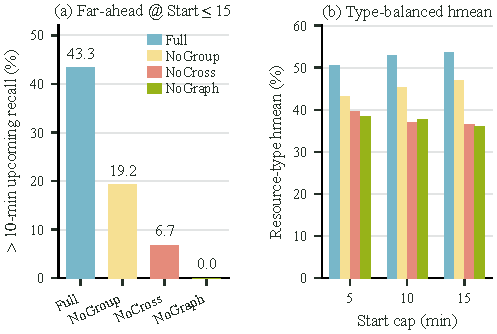
\includegraphics[width=\columnwidth]{figures/fig_cross_resource_evidence.pdf}
\caption{Cross-resource evidence from structural ablations: (a)~far-onset report recall at Start$\leq15$; (b)~type-hmean F1 across Start caps.}
\label{fig:cross-resource-evidence}
\end{figure}

\begin{figure*}[t]
\centering
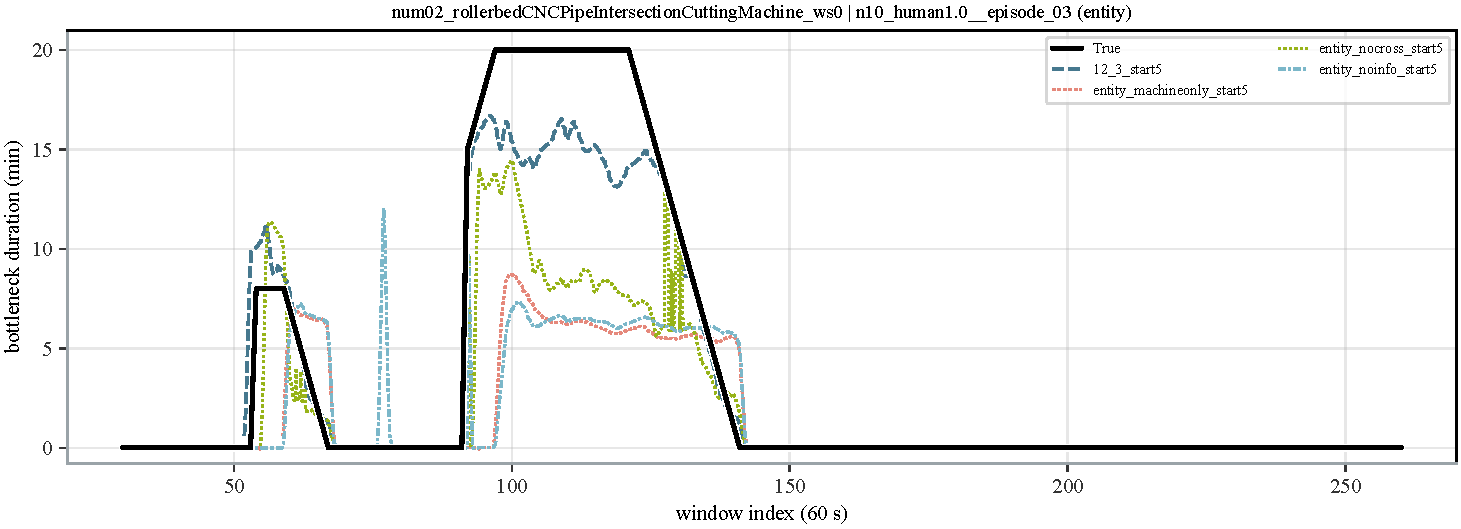
\includegraphics[width=0.96\textwidth]{figures/key_device_entity.pdf}
\caption{Key-device duration traces: (a)~multi-entity ablations at Start$\leq5$; (b)~PHGST-DM under Start$\leq5/10/15$ on the same episode.}
\label{fig:key-device-entity}
\end{figure*}

\paragraph*{Learned cross-resource allocation under mixed operating conditions.}
Attention sampling and averaging follow the protocol in Section~\ref{sec:attention-protocol}. Figure~\ref{fig:attn-change} retains the resource-level change maps underlying the main-text type summary.

Upcoming and ongoing averages are compared with normal attention. Colour indicates increased or decreased weight; the absolute reference matrices are retained below.

\begin{figure*}[pos=!htbp]
\centering
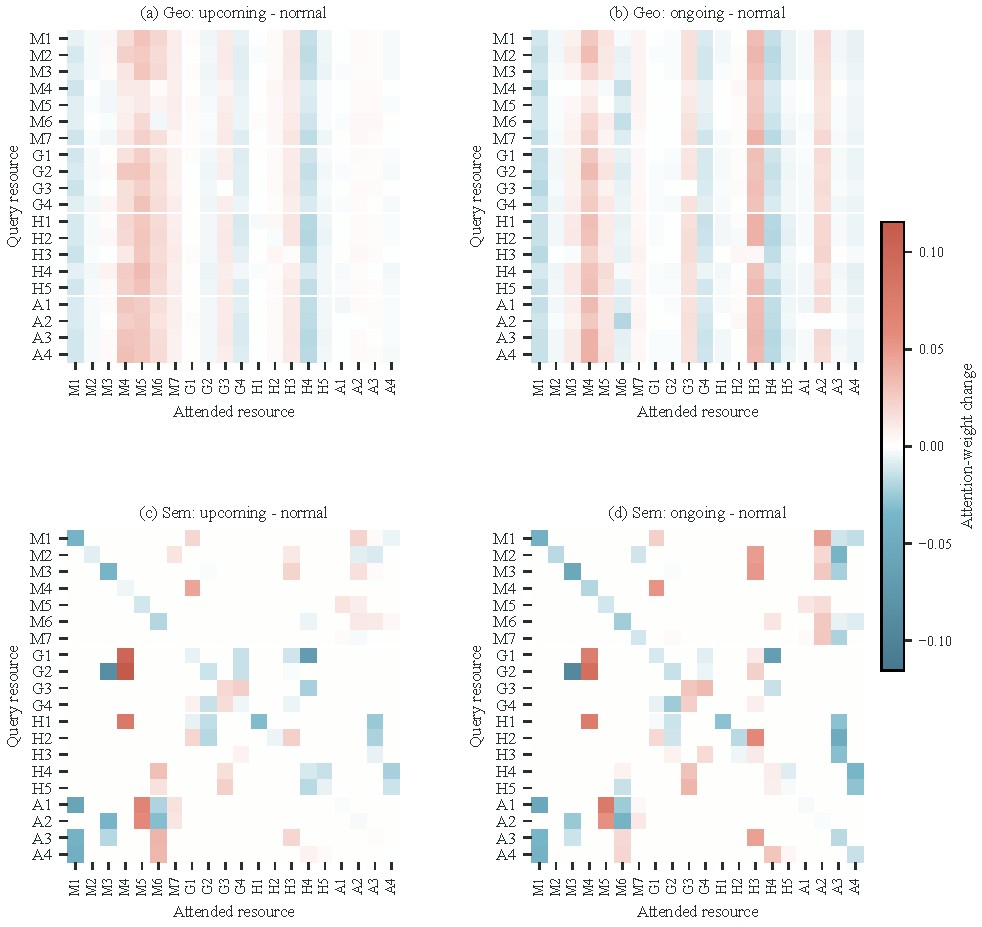
\includegraphics[width=0.92\textwidth]{figures/attention_heatmaps/fig03_resource_attention_change.pdf}
\caption{Resource-attention redistribution relative to normal for upcoming and ongoing samples (coral: increase; blue: decrease).}
\label{fig:attn-change}
\end{figure*}



\subsubsection{Process-informed supervision and temporal pattern clustering}\label{sec:supervision-analysis}
% Prefer text+float sharing a column page; avoid near-empty float pages.
\setcounter{topnumber}{3}
\setcounter{bottomnumber}{2}
\setcounter{totalnumber}{5}
\renewcommand{\topfraction}{0.9}
\renewcommand{\bottomfraction}{0.8}
\renewcommand{\textfraction}{0.15}
\renewcommand{\floatpagefraction}{0.75}
\renewcommand{\dbltopfraction}{0.9}

Process-informed supervision connects the event representation to production meaning. The analysis focuses on temporal pattern clustering, cause accuracy under a matched training budget, and alignment between process-informed label rankings and intervention-sensitive resources. These experiments answer different questions and are therefore interpreted separately.

\zhpara{过程知情监督将事件表示与生产意义联系起来。本节从三个层面展开：完整监督配置下的事件与状态报告、统一训练预算下的原因准确率，以及过程知情标签排序与干预敏感资源之间的对齐。三组实验回答不同问题，因此分别解释。}

\paragraph*{(1) Effects of temporal pattern clustering.}
NoCluster removes temporal pattern clustering to assess its contribution to recurrent temporal-pattern prototype construction. NoPattern separately disables the use of prototype matching in delay-aware modeling.

\zhpara{\paragraph*{(1) 时间模式聚类的作用。}
NoCluster 去掉时间模式聚类，以评估其对重复时间模式原型构造的贡献。NoPattern 则单独关闭延迟感知建模中的原型匹配。}

\begin{table*}[t]
\centering
\caption{Event, state, and duration metrics for the Full configuration and NoCluster (temporal pattern clustering removed). Dur.\ MAE is the union error (min); Dur.\ MAE (tp) is computed on correctly reported events only.}
\label{tab:group-ablation}
\scriptsize
\setlength{\tabcolsep}{3.5pt}
\renewcommand{\arraystretch}{1.08}
\begin{tabular*}{\FullWidth}{@{\extracolsep{\fill}}llrrrrr@{}}
\toprule
Arm & Start cap & F1-score & Upcoming R & State F1 (1-step) & Dur.\ MAE & Dur.\ MAE (tp) \\
\midrule
Full & $\leq5$ & \textbf{80.4\%} & \textbf{54.2\%} & \textbf{88.3\%} & \textbf{4.17} & \textbf{1.86} \\
NoCluster & & 73.4\% & 12.5\% & 84.1\% & 5.43 & 2.89 \\
\midrule
Full & $\leq10$ & \textbf{77.8\%} & \textbf{53.5\%} & \textbf{89.2\%} & \textbf{4.38} & \textbf{1.79} \\
NoCluster & & 57.0\% & 34.6\% & 78.9\% & 6.69 & 2.40 \\
\midrule
Full & $\leq15$ & \textbf{76.8\%} & \textbf{53.7\%} & \textbf{90.0\%} & \textbf{4.43} & \textbf{1.72} \\
NoCluster & & 53.7\% & 37.3\% & 81.9\% & 6.65 & 2.30 \\
\bottomrule
\end{tabular*}
\end{table*}

\paragraph*{(2) Effects of cause supervision.}
Cause supervision improves prediction of the rule-derived process-cause labels under matched training conditions (Table~\ref{tab:matched-cause}). With PHGST-DM labels, a common data split, Start$\leq5$, seed 42, random initialization, and a 50-epoch budget, logged cause accuracy rises from $19.5\%$ to $89.5\%$, and the separately selected cause accuracy and macro recall rise from $25.2\%/25.5\%$ to $92.2\%/93.7\%$. Logged station F1 remains near $73\%$, so the measured benefit is localized to the explanatory output.

\zhpara{统一训练条件下，原因监督直接提升了过程解释能力（表~\ref{tab:matched-cause}）。固定 Ops 标签、数据划分、Start$\leq5$、seed 42、随机初始化和五十个 epoch 的预算后，日志原因准确率由 $19.5\%$ 升至 $89.5\%$，另行选定的原因准确率与宏召回由 $25.2\%/25.5\%$ 升至 $92.2\%/93.7\%$；日志工位 F1 仍接近 $73\%$，因此实测收益主要位于解释输出。}

\begin{table}[pos=htbp]
\centering
\caption{Matched-budget cause-supervision study at Start$\leq5$ (seed 42; 50 epochs). Values are percentages. Logged metrics come from the training export; selected cause metrics use a separately chosen operating point and are not interchanged with the logged values.}
\label{tab:matched-cause}
\scriptsize
\setlength{\tabcolsep}{3.5pt}
\renewcommand{\arraystretch}{1.08}
\begin{tabular*}{\columnwidth}{@{\extracolsep{\fill}}lrr@{}}
\toprule
Metric & Backbone & +Cause \\
\midrule
Logged station F1 & 73.5\% & 73.3\% \\
Logged cause acc. & 19.5\% & \textbf{89.5\%} \\
Selected cause acc. & 25.2\% & \textbf{92.2\%} \\
Selected cause macro recall & 25.5\% & \textbf{93.7\%} \\
\bottomrule
\end{tabular*}
\end{table}

% Evidence: isaac_factory origin/dev_tyx, 8767583f3ed6392cfd8061d4a80de94fcfb9d7a0.
% Source: bottleneck ground-truth validity notes (2026-10-14), checked against label/evaluation code.
% Imported summary values: experiments/data/label_validity_dev_tyx_8767583.json.
\paragraph*{(3) Validation against production sensitivity.}
Production sensitivity provides an operational criterion for bottleneck labels: prioritizing resources whose temporary acceleration shortens order completion. Counterfactual replay compares a service intervention with the unchanged production trajectory from the same saved state. This connects the label ranking to the consequence of a resource-level action.

At a saved factory-model state $t$, each of seven workstation candidates receives a separate service-bundle intervention. Workstation processing and its associated worker service use a duration scale of $0.8$, equivalent to a $1.25\times$ service rate, for 1,200 model steps. Baseline and intervention branches start from the same saved state and random-number state and run to order completion. The counterfactual sensitivity is
\begin{equation}
S_i(t)=M_{\mathrm{base}}(t)-M_{i,0.8}(t),
\end{equation}
where $M$ denotes order-completion time. Positive $S_i(t)$ indicates that temporarily accelerating resource $i$ shortens the order. Each label method ranks candidates using its maximum evidence over the last three fully observed windows before $t$.

\zhpara{在保存的仿真状态 $t$，分别对七个候选机器或工位施加服务组合干预：机器加工及其关联人工作业采用 $0.8$ 的时长缩放系数，即 $1.25$ 倍服务速率，持续 1,200 个仿真步。基准分支与干预分支从相同的保存状态和随机数状态出发，运行至订单完成。反事实敏感度定义为 $S_i(t)=M_{\mathrm{base}}(t)-M_{i,0.8}(t)$，其中 $M$ 表示订单完成时间；$S_i(t)>0$ 表示临时加速资源 $i$ 能缩短订单完成时间。各标签方法使用 $t$ 之前最近三个完整观测窗口内的最大证据值对候选资源排序。}

PHGST-DM yields the highest point estimates on all five sensitivity-alignment metrics in the three-episode nominal-condition pilot (Figure~\ref{fig:label-oracle-pilot}). NDCG@3 measures ranking quality using positive sensitivity as relevance; Positive Recall@$k$ measures coverage of the oracle's $k$ highest positive-sensitivity resources by the first $k$ candidates. Weighted Recall@3 gives the fraction of total positive sensitivity captured by the first three candidates, and Coverage@3$_{0.9}$ covers resources satisfying $S_i\geq0.9\max_j S_j$. PHGST-DM reaches NDCG@3 $0.531$ and Weighted Recall@3 $0.716$, compared with $0.495$ and $0.585$ for Queue-Wait. The mean weighted coverage of positive sensitivity by its top-three candidates is $71.6\%$ under this pilot protocol. Early-, middle-, and late-stage NDCG@3 values are $0.421/0.339/0.770$, with the strongest alignment near order completion.

\zhpara{在三个无扰动 episode 的先导实验中，Ops 的五项敏感度对齐指标点估计均最高（图~\ref{fig:label-oracle-pilot}）。NDCG@3 以正敏感度为相关性衡量排序质量，Positive Recall@$k$ 衡量前 $k$ 个候选对 oracle 中正敏感度最高的 $k$ 个资源的覆盖。Weighted Recall@3 表示前三候选覆盖的正敏感度占总正敏感度的比例，Coverage@3$_{0.9}$ 则评价对满足 $S_i\geq0.9\max_j S_j$ 的资源的覆盖。Ops 的 NDCG@3 为 $0.531$，Weighted Recall@3 为 $0.716$，Queue-Wait 对应为 $0.495$ 和 $0.585$；在该先导实验协议下，Ops 前三候选对正敏感度的平均加权覆盖率为 $71.6\%$。生产早期、中期和后期的 NDCG@3 为 $0.421/0.339/0.770$，在订单接近完成时对齐程度最高。}

\begin{figure}[pos=htbp]
\centering
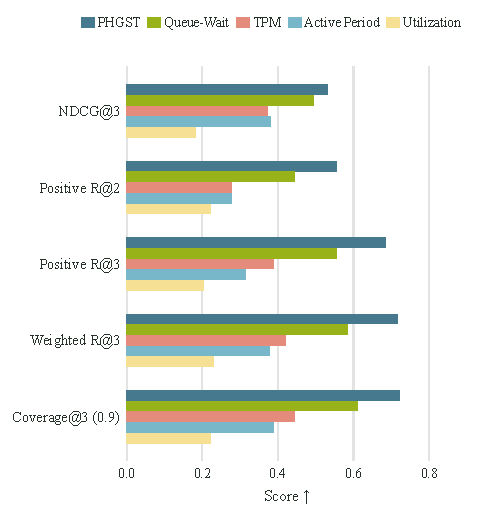
\includegraphics[width=\columnwidth]{figures/fig_label_oracle_bars.pdf}
\caption{Counterfactual sensitivity alignment in the exploratory pilot (↑ better).}
\label{fig:label-oracle-pilot}
\end{figure}

These exploratory estimates support production sensitivity as a distinct dimension of supervision quality. All five retained soft-alignment metrics favour PHGST-DM in this pilot, but the metric set was finalized after inspecting the pilot and Holm-adjusted paired comparisons do not reject the null hypotheses. The independent full-Oracle evaluation has not been run; the numerical ordering is therefore interpreted only as a development result for nominal-condition episodes, not as proof of general superiority across operating conditions.

\zhpara{这些探索性估计支持将生产敏感度作为监督质量的独立评价维度。五项保留的软对齐指标在该先导实验中均由 Ops 取得最高点估计，但指标集合是在查看先导结果后确定的，经 Holm 校正的配对比较也未拒绝零假设。独立 full-Oracle 评价尚未运行，因此当前数值排序只能解释为无扰动 episode 上的开发结果，不能作为跨工况普遍最优的证据。}

\subsubsection{Delay-aware modeling}

Temporal pattern clustering supplies the recurrent prototype bank, while delay-aware modeling uses that bank to support warnings that precede the visible bottleneck state. PHGST-DM records Upcoming recall of $0.542/0.535/0.537$, compared with $0.167/0.278/0.427$ for NoPattern, which retains the graph and attention branches while disabling the matching of recent patches to the temporal-pattern prototype bank (Table~\ref{tab:delay-ablation-new}). For events starting more than 10~min ahead, strict report recall is $0.433$ versus $0.163$. This distance-resolved result is consistent with the role of prototype-conditioned historical context in representing delayed propagation. Cause macro recall is $0.967/0.965/0.978$ for Full and $0.734/0.805/0.850$ for NoPattern; the largest class-level contrast is queue buildup, with recall $0.984$ versus $0.145$ at Start$\leq5$. The stage-1 remaining-time reference also records MAE $10.93/11.21/9.72$~min, compared with $18.62/13.35/11.06$~min for NoPattern, linking temporal context to order-progress estimation.

\zhpara{延迟感知建模支持在可见瓶颈状态形成之前发出预警。PHGST-DM 的 Upcoming 召回率为 $0.542/0.535/0.537$，NoPattern 为 $0.167/0.278/0.427$；后者保留工厂图和注意力分支，关闭近期片段与聚类模式键的匹配（表~\ref{tab:delay-ablation-new}）。对于十分钟以后才开始的事件，严格报告召回率为 $0.433$ 对 $0.163$，这一距离分解结果与历史模式用于表征延迟传播的作用一致。Full 的原因宏平均召回率为 $0.967/0.965/0.978$，NoPattern 为 $0.734/0.805/0.850$；其中差异最大的队列积压类别在 Start$\leq5$ 下为 $0.984$ 对 $0.145$。第一阶段模型的剩余时间 MAE 为 $10.93/11.21/9.72$ 分钟，NoPattern 为 $18.62/13.35/11.06$ 分钟，进一步将时间上下文与订单进度估计联系起来。}

\begin{table*}[t]
\centering
\caption{Ablation of temporal-pattern prototype matching in delay-aware modeling. $R_{\mathrm{up,rep}}$ is strict report recall within the stated onset-distance bin; Cause Macro R is macro recall over the four supported process-cause classes. Remain MAE (min) is compared with the stage-1 model, which, like the ablation, has no remaining-time fine-tuning.}
\label{tab:delay-ablation-new}
\scriptsize
\setlength{\tabcolsep}{2.6pt}
\renewcommand{\arraystretch}{1.08}
\begin{tabular*}{\FullWidth}{@{\extracolsep{\fill}}llrrrrrrr@{}}
\toprule
Arm & Start cap & F1-score & Upcoming R & $R_{\mathrm{up,rep}}^{6\text{--}10}$ & $R_{\mathrm{up,rep}}^{>10}$ & Queue R & Cause Macro R & Remain MAE \\
\midrule
Full (stage 1) & $\leq5$ & \textbf{80.4\%} & \textbf{54.2\%} & --- & --- & \textbf{98.4\%} & \textbf{96.7\%} & \textbf{10.93} \\
NoPattern & & 74.5\% & 16.7\% & --- & --- & 14.5\% & 73.4\% & 18.62 \\
\midrule
Full (stage 1) & $\leq10$ & \textbf{77.8\%} & \textbf{53.5\%} & \textbf{46.6\%} & --- & \textbf{98.4\%} & \textbf{96.5\%} & \textbf{11.21} \\
NoPattern & & 58.8\% & 27.8\% & 14.9\% & --- & 47.6\% & 80.5\% & 13.35 \\
\midrule
Full (stage 1) & $\leq15$ & \textbf{76.8\%} & \textbf{53.7\%} & \textbf{52.2\%} & \textbf{43.3\%} & \textbf{98.4\%} & \textbf{97.8\%} & \textbf{9.72} \\
NoPattern & & 60.1\% & 42.7\% & 39.6\% & 16.3\% & 57.3\% & 85.0\% & 11.06 \\
\bottomrule
\end{tabular*}
\end{table*}

\paragraph*{Historical and layer-wise attention structure.}
Figures~\ref{fig:attn-temporal}--\ref{fig:attn-horizons} examine temporal context within the same supplementary mixed-disturbance analysis. Figure~\ref{fig:attn-temporal} covers all 30 historical windows under normal and upcoming conditions, with an upcoming-minus-normal panel that resolves smaller shifts in the historical positions receiving attention. Its difference scale is much narrower than the absolute-weight scale, so the panel should not be read as a large change in temporal dependence. Figure~\ref{fig:attn-layers} focuses the main-text comparison on encoder layers 1, 4, and 5, retaining an input-near layer and the final two layers while keeping both geographic and semantic branches readable. The complete five-layer view is retained in Appendix~\ref{app:layerwise-attention}. Layer-specific weights do not measure the accuracy contribution of each layer.

Figure~\ref{fig:attn-horizons} compares the upcoming-minus-normal resource maps from three separately trained Start$\leq5/10/15$ mixed-disturbance checkpoints, with 96 samples per condition and checkpoint. The persistent structure and localized changes provide a descriptive view across onset settings. They neither trace propagation through physical time nor replace the distance-resolved recall comparison in Table~\ref{tab:delay-ablation-new}.

\begin{figure*}[t]
\centering
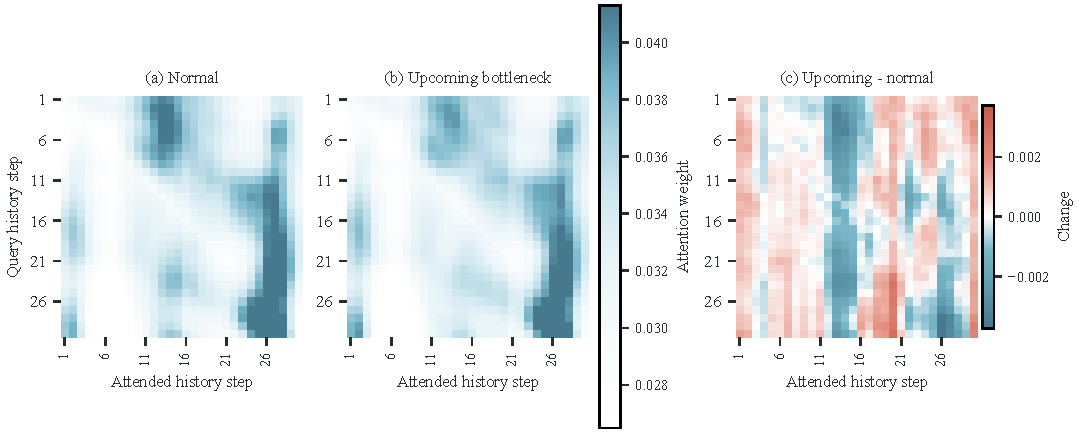
\includegraphics[width=0.98\textwidth]{figures/attention_heatmaps/fig04_temporal_attention_states.pdf}
\caption{Temporal attention over 30 history windows: (a)~normal; (b)~upcoming; (c)~upcoming-minus-normal.}
\label{fig:attn-temporal}
\end{figure*}
\begin{figure*}[t]
\centering
\includegraphics[width=0.92\textwidth]{figures/attention_heatmaps/fig05_layerwise_upcoming_attention_selected.pdf}
\caption{Geographic (upper) and semantic (lower) attention in selected encoder layers 1, 4, and 5.}
\label{fig:attn-layers}
\end{figure*}
\begin{figure*}[t]
\centering
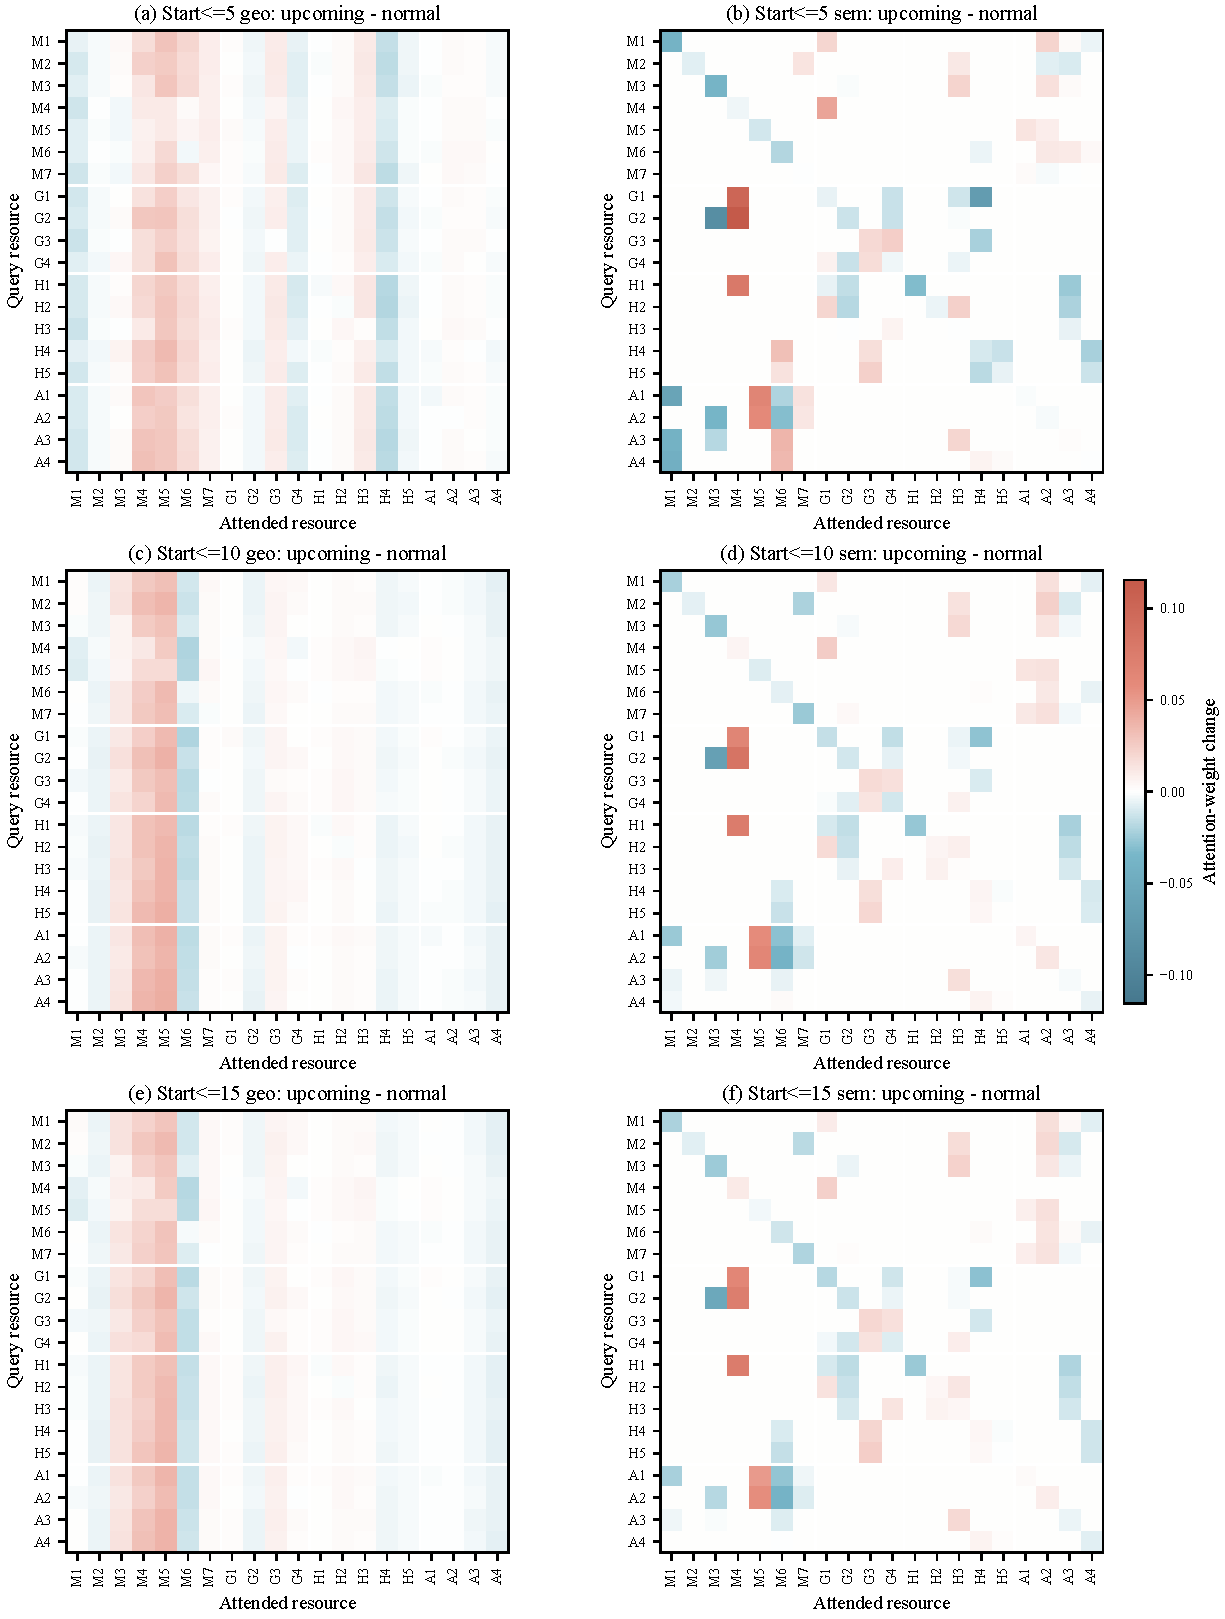
\includegraphics[width=0.98\textwidth]{figures/attention_heatmaps/fig07_horizon_attention_change.pdf}
\caption{Upcoming-minus-normal attention change across Start caps 5/10/15 (upper: geographic; lower: semantic).}
\label{fig:attn-horizons}
\end{figure*}


\subsubsection{Decoder and training components}\label{sec:decoder-training}

The decoder and training comparisons examine two requirements of advance warning: distinguishing new events from continuing events and maintaining sensitivity to distant onsets. NoSplit replaces the continuation and onset heads with one shared head, while NoFarBoost removes far-onset weighting and the associated enhanced false-alarm penalty. Both arms retain the common initialization, 50-epoch curriculum, and validation-controlled checkpoint and threshold-selection rule. Table~\ref{tab:decoder-ablation} reports the resulting operating points.

\zhpara{解码器与训练比较考察提前预警的两项要求：区分新事件与持续事件，以及保持对较远开始时刻的敏感性。NoSplit 用单一共享头替换继续头与开始头；NoFarBoost 去除远开始加权及相关的强化误报惩罚。两个分支均保留共用初始化、50 个 epoch 课程以及验证控制的检查点与阈值选择规则。表~\ref{tab:decoder-ablation}报告相应工作点。}

\begin{table*}[t]
\centering
\caption{Ablation of the split event heads and the far-onset enhancement. Distance-specific $R_{\mathrm{up,rep}}$ additionally requires the three-window onset tolerance. Thr is the validation-selected report threshold.}
\label{tab:decoder-ablation}
\scriptsize
\setlength{\tabcolsep}{3.5pt}
\renewcommand{\arraystretch}{1.08}
\begin{tabular*}{\FullWidth}{@{\extracolsep{\fill}}llrrrrrr@{}}
\toprule
Arm & Start cap & Thr & F1-score & Upcoming R & $R_{\mathrm{up,rep}}^{>10}$ & Ongoing R & Dur.\ MAE \\
\midrule
Full & $\leq5$ & 94.0\% & 80.4\% & 54.2\% & --- & \textbf{93.7\%} & 4.17 \\
NoFarBoost & & 90.0\% & \textbf{81.9\%} & \textbf{54.5\%} & --- & 92.3\% & \textbf{4.03} \\
NoSplit & & 94.0\% & 72.7\% & 19.0\% & --- & 93.5\% & 5.56 \\
\midrule
Full & $\leq10$ & 94.0\% & \textbf{77.8\%} & 53.5\% & --- & 93.9\% & \textbf{4.38} \\
NoFarBoost & & 88.0\% & 75.2\% & \textbf{56.0\%} & --- & 92.3\% & 4.66 \\
NoSplit & & 94.0\% & 58.0\% & 24.7\% & --- & \textbf{94.7\%} & 6.63 \\
\midrule
Full & $\leq15$ & 94.0\% & \textbf{76.8\%} & \textbf{53.7\%} & \textbf{43.3\%} & 93.0\% & \textbf{4.43} \\
NoFarBoost & & 94.0\% & 74.1\% & 48.9\% & 24.0\% & 92.5\% & 4.87 \\
NoSplit & & 94.0\% & 58.6\% & 35.3\% & 12.5\% & \textbf{95.1\%} & 6.36 \\
\bottomrule
\end{tabular*}
\end{table*}

Separating onset and continuation decisions gives PHGST-DM Upcoming recall of $0.542/0.535/0.537$, compared with $0.190/0.247/0.353$ for the shared head; NoSplit's Ongoing recall remains $0.935$--$0.951$. The contrast localizes the value of separate decisions to emerging events. Far-onset enhancement concentrates its benefit at the 10- and 15-min caps, where PHGST-DM records F1-score $0.778/0.768$ and union duration MAE $4.38/4.43$~min, compared with $0.752/0.741$ and $4.66/4.87$~min for NoFarBoost. Strict report recall for events beyond 10~min rises from $0.240$ to $0.433$. At the 5-min cap, NoFarBoost records F1-score $0.819$ and union MAE $4.03$~min, at threshold $0.90$ versus $0.94$ for PHGST-DM. This range-dependent pattern motivates the enhancement for longer warning distances. On the key-device trace (Figure~\ref{fig:key-device-struct-graph}), PHGST-DM reaches 15--17~min during the displayed 20-min reference plateau and follows its decay; the structural variants peak at 12--14.5~min and show post-event spikes.

\zhpara{分离起点与持续判定后，PHGST-DM 的 Upcoming 召回率为 $0.542/0.535/0.537$，共享头为 $0.190/0.247/0.353$，而 NoSplit 的 Ongoing 召回率保持在 $0.935$--$0.951$。这一对照将分离判定的价值定位到正在形成的事件。远期增强的收益集中在十分钟和十五分钟范围：PHGST-DM 的 F1-score 为 $0.778/0.768$，union 持续时间 MAE 为 $4.38/4.43$ 分钟，NoFarBoost 对应为 $0.752/0.741$ 和 $4.66/4.87$ 分钟；对十分钟以后事件的严格报告召回率从 $0.240$ 提高到 $0.433$。五分钟范围下，NoFarBoost 的 F1-score 为 $0.819$、union MAE 为 $4.03$ 分钟，其阈值为 $0.90$，PHGST-DM 为 $0.94$。这种随范围变化的结果支持将远期增强用于更长预警距离。关键设备轨迹（图~\ref{fig:key-device-struct-graph}和图~\ref{fig:key-device-struct-mech}）中，PHGST-DM 在所示二十分钟参考平台期内达到 15--17 分钟并跟随其下降，结构变体的峰值为 12--14.5 分钟，并出现事件结束后的尖峰。}

Head-specific stage-2 fine-tuning reduces overall order remaining-time MAE by $1.32/1.94/0.81$~min at Start$\leq5/10/15$, respectively (Figure~\ref{fig:remain-finetune}). The phase-resolved comparison shows that the reduction is concentrated in early production, where MAE falls by $2.70/3.49/1.64$~min, and remains positive in the middle phase. Late-production MAE changes by only $+0.09/-0.13/+0.01$~min, indicating that the aggregate gain comes primarily from the more difficult early and middle windows rather than a uniform shift across the order trajectory. The event and cause heads remain frozen during this fine-tuning stage.

\zhpara{针对剩余时间预测头的第二阶段专项微调，使 Start$\leq5/10/15$ 下的订单剩余时间总体 MAE 分别下降 $1.32/1.94/0.81$ 分钟（图~\ref{fig:remain-finetune}）。分阶段结果表明，收益主要集中在生产早期，此时 MAE 分别下降 $2.70/3.49/1.64$ 分钟；中期也保持正向改善。生产晚期的 MAE 仅变化 $+0.09/-0.13/+0.01$ 分钟，说明总体收益主要来自更困难的早期和中期窗口，而不是整段订单过程的一致平移。该阶段保持事件头与原因头冻结。}

\begin{figure*}[t]
\centering
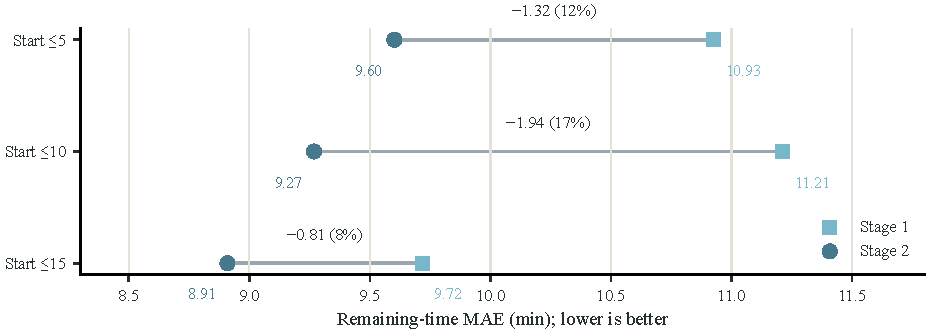
\includegraphics[width=0.90\textwidth]{figures/fig_remain_dumbbell.pdf}
\caption{Effect of remaining-time fine-tuning across early, middle, and late production phases (blue: MAE decrease; coral: increase).}
\label{fig:remain-finetune}
\end{figure*}
\begin{figure*}[t]
\centering
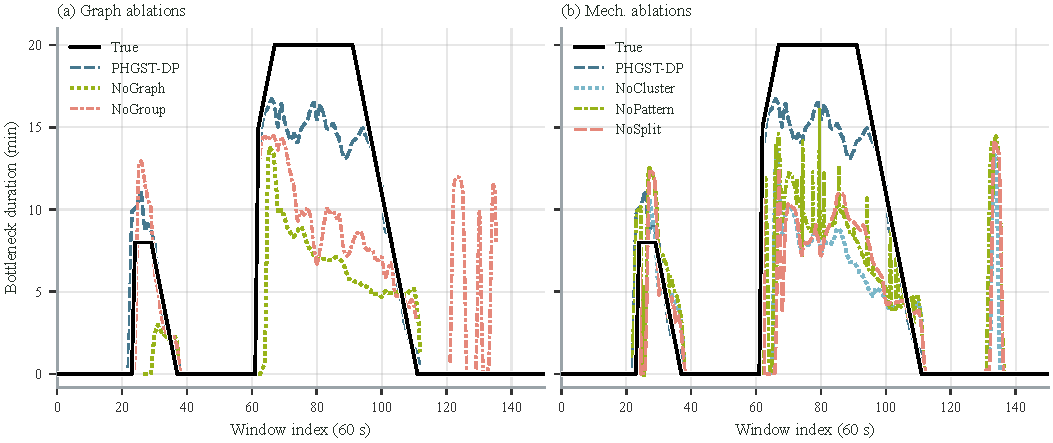
\includegraphics[width=0.96\textwidth]{figures/key_device_struct_pair.pdf}
\caption{Key-device ablation traces (Start$\leq5$): (a)~graph arms; (b)~process-rule/context, delay-aware modeling, and decoder arms.}
\label{fig:key-device-struct-graph}
\end{figure*}

\paragraph*{Supplementary development diagnostics.}


\subsection{Case study and process traceability}

The case study shows how an event report follows bottleneck onset, persistence, and recovery on a production resource. The selected roller-bed CNC pipe-intersection cutting workstation (\texttt{num02}) contributes 301 event-positive window--resource pairs in the test set. Device and episode selection follows a fixed rule: among devices with at least the median event count, select the device with the most events in one episode (ties resolved by PHGST-DM one-step F1), then select its episode with the most and longest bottleneck segments. The resulting episode, \texttt{n10\_human1.0\_\_episode\_03}, contains an approximately 8-min bottleneck and a 49-min bottleneck. The prediction horizon remains 30~min. For visualization, the true-duration reference in the key-device plots is truncated at 20~min to emphasize onset and recovery; the omitted 20--30~min range does not change the experimental prediction horizon. PHGST-DM detects both intervals and tracks their recovery (Figure~\ref{fig:key-device-baselines}). The short event is reported about 1~min in advance with a 10--11~min duration estimate; the long event's onset is aligned, and its declining duration is followed. During the displayed reference plateau, predicted duration is 13--17~min, and state mismatches occur at onset and recovery boundaries (1--2 windows each). The trace illustrates how the report combines event notification with a continuously updated duration estimate.

\zhpara{案例展示事件报告如何跟踪生产资源上瓶颈的发生、持续与恢复。所选滚床数控相贯线切割机（\texttt{num02}）在测试集中贡献 301 个事件阳性窗口—资源对。设备与 episode 依据固定规则选择：在事件数不低于中位数的设备中，选取单个 episode 内事件数最多的设备，并列时依据 PHGST-DM 单步 F1 确定；再选择该设备瓶颈段数最多、持续时间最长的 episode。得到的 \texttt{n10\_human1.0\_\_episode\_03} 包含约八分钟和四十九分钟的两个瓶颈。预测范围仍为三十分钟；关键设备图中的真实持续时间参考为突出起点与恢复而截断在二十分钟，省略的 20--30 分钟区间不改变实验预测范围。PHGST-DM 识别出两个区间并跟踪其恢复过程（图~\ref{fig:key-device-main}）：短事件提前约一分钟报告，持续时间估计为 10--11 分钟；长事件的起点对齐，持续时间下降段得到跟踪。封顶区间的预测为 13--17 分钟，状态错分发生在起点与恢复边界，各为 1--2 个窗口。该轨迹展示了事件通知与持续更新的时间估计如何共同组成预测报告。}

\begin{figure*}[t]
\centering
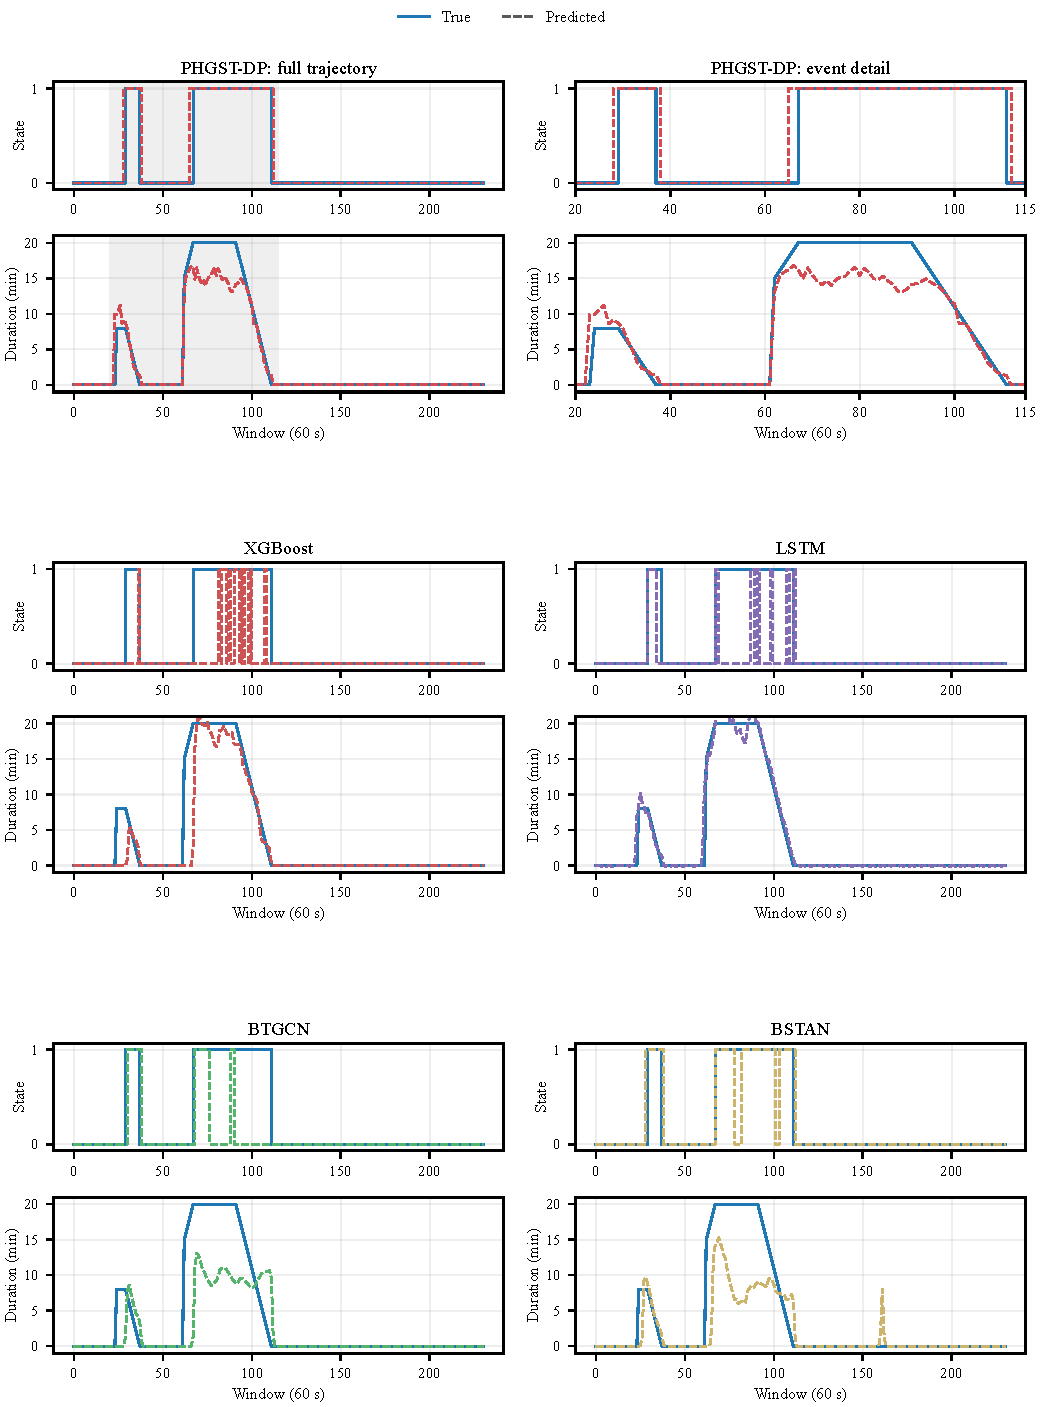
\includegraphics[width=0.96\textwidth]{figures/key_device_models_aligned.pdf}
\caption{Key-device comparison of PHGST-DM and baselines at Start$\leq5$: (a)~next-window state; (b)~duration with the true reference truncated at 20~min for visualization (black: true; dashed: predictions).}
\label{fig:key-device-baselines}
\end{figure*}

Figure~\ref{fig:key-device-baselines} overlays PHGST-DM with XGBoost, LSTM, BTGCN, and BSTAN on the same device and episode: next-window state on the left and duration on the right. Black solid lines show the targets; dashed predictions use one colour per method. Window indices start after the 30-window history. PHGST-DM maintains continuous state coverage over both bottleneck intervals and follows the duration decline towards recovery, while the baselines show gaps or weaker duration tracking on the same trajectory. The aggregate event and temporal results are reported in Table~\ref{tab:comparison-main}.

\zhpara{图~\ref{fig:key-device-baselines}在同一设备与同一 episode 上将 PHGST-DM 与 XGBoost、LSTM、BTGCN、BSTAN 叠加对比：左侧为下一窗口状态，右侧为持续时间。黑色实线为目标；各方法预测以虚线并用不同颜色区分。窗口索引从 30 窗口历史之后开始计数。PHGST-DM 在两段瓶颈区间上保持连续状态覆盖，并跟随持续时间向恢复下降；基线在同一轨迹上则出现缺口或更弱的持续时间跟踪。总体事件与时间结果见表~\ref{tab:comparison-main}。}

The all-resource view connects these local traces to coordinated production-state prediction. Figure~\ref{fig:all-devices-main} shows the seven workstation targets in the same episode. That episode contains 64 positive bottleneck cells, the highest count among test episodes, and all of them fall on these workstations. PHGST-DM recovers every positive cell of the cutting workstation and second welding station (\texttt{num00\_weld\_ws1}), with episode-level State F1 $0.941$. Light-blue cells denote true positives; red cells denote false positives and false negatives. The corresponding F1 values are $0.855$ for NoInfo, $0.832$ for NoCluster, and $0.901$ for NoGraph. NoInfo and NoCluster omit the welding-station interval, while NoGraph fragments it. In this episode, the full model maintains coverage across both resources, while the ablated variants miss or fragment the welding-station interval.

\zhpara{全资源视图将局部轨迹扩展为协同生产状态预测。图~\ref{fig:all-devices-main}给出同一 episode 的七个机器与工作台目标。该 episode 含 64 个正例瓶颈格子，为测试 episode 中最多，且全部落在这些机器上。PHGST-DM 覆盖切割机和第二焊接工位（\texttt{num00\_weld\_ws1}）的全部正例格子，episode 级 State F1 为 $0.941$。浅蓝色表示真阳性，红色表示假阳性与假阴性。NoInfo、NoCluster 和 NoGraph 的对应 F1 为 $0.855$、$0.832$ 和 $0.901$；NoInfo 与 NoCluster 漏报焊接工位区间，NoGraph 将其切分为片段。完整模型对两个资源的连续覆盖，直观呈现了资源信息、监督与图结构在生产状态报告中的共同作用。}

\begin{figure}[pos=htbp]
\centering
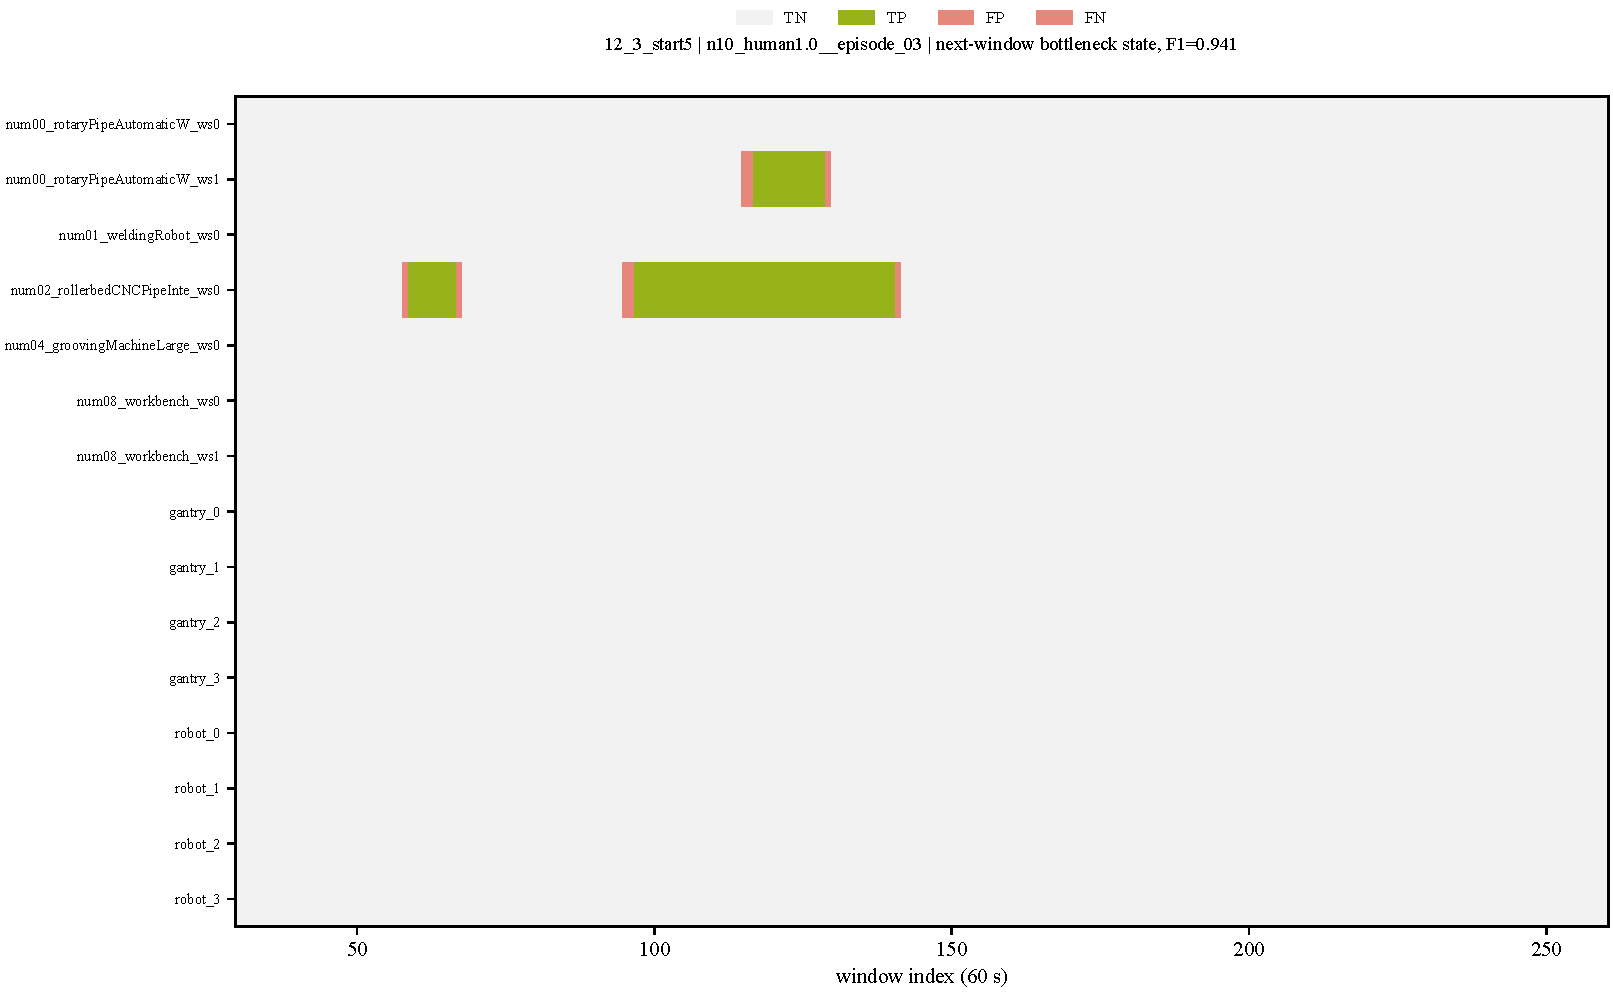
\includegraphics[width=\columnwidth]{figures/all_devices_state_main.pdf}
\caption{Next-window state map for seven workstation targets (gray TN; light blue TP; coral FP/FN).}
\label{fig:all-devices-main}
\end{figure}

On the full Start$\leq5$ test split, support is uneven across the 15 targets (Figure~\ref{fig:per-device}). The cutting workstation contributes 301 true events, while AGV~2 and AGV~3 contribute none and are excluded from the box statistics. F1 on the supported devices ranges from $0.535$ on the welding robot to $0.964$ on bench~ws1. This split is a coverage check for one checkpoint, not a claim that every resource family is equally predictable.

\zhpara{在完整的 Start$\leq5$ 测试划分上，十五个目标的支持量并不均匀（图~\ref{fig:per-device}）。切割机有 301 个真实事件，而 robot~2 与 robot~3 没有真实事件，不进入箱线统计。有支持设备的 F1 从焊接机器人的 $0.535$ 到 bench~ws1 的 $0.964$。该图只检查一个 checkpoint 的覆盖情况，不能据此认为每一类资源都同样可预测。}

\begin{figure*}[t]
\centering
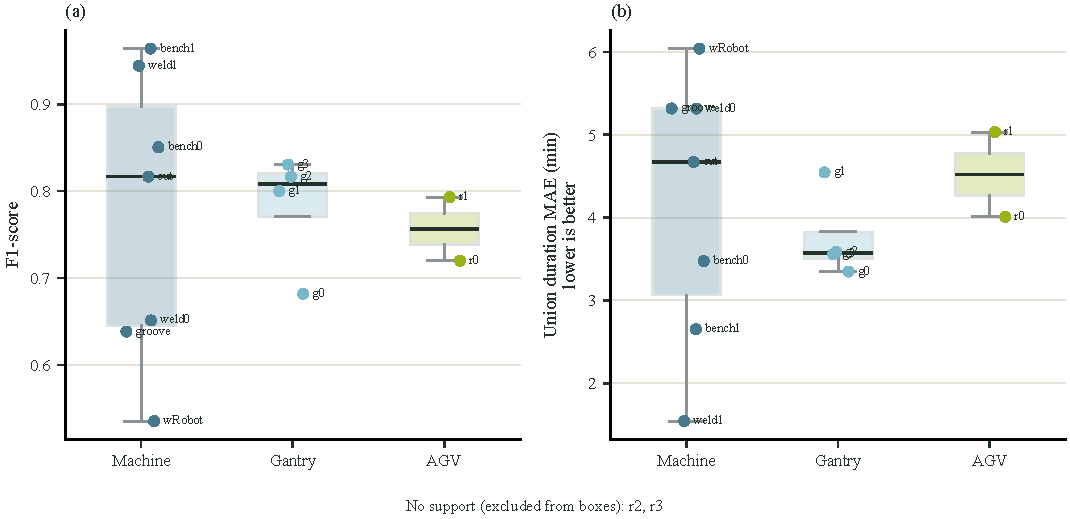
\includegraphics[width=0.96\textwidth]{figures/fig_per_device_box.pdf}
\caption{Per-device F1-score and union duration MAE for PHGST-DM at Start$\leq5$, by workstation, gantry, and AGV.}
\label{fig:per-device}
\end{figure*}

Process-cause outputs link a predicted event to interpretable production symptoms: material shortage, transport delay, queue buildup, and downstream blockage. The labels encode process-rule evidence, so the explanation is an association with observed operating conditions. Together with the event and state traces, these outputs provide a resource, a time interval, and a process context for reviewing a predicted constraint.

\zhpara{过程原因输出把所预测事件与可解释生产症状联系起来：物料短缺、运输延迟、队列积压与下游阻塞。标签编码过程规则证据，因此解释是与所观测运行条件的关联。连同事件与状态轨迹，这些输出为审视所预测约束提供资源、时间区间与过程上下文。}

\paragraph*{Mixed-condition probability map.}
Figure~\ref{fig:attn-prediction} extends the single-resource trajectory to a supplementary mixed-condition episode, \texttt{n10\_mix\_all1.0\_\_episode\_03}. It is selected automatically for high bottleneck activity and displays relative test-window indices $0$--$200$ from the Start$\leq5$ mixed-condition checkpoint. The three aligned panels retain the future-event labels, model probabilities and absolute probability errors. Visible mismatches include probabilities on resources without a corresponding positive label as well as incomplete coverage of labelled intervals. The probability map is distinct from a thresholded operational report. Its 20 displayed rows contain the 15 evaluation targets and five worker context nodes; the 18 buffer rows are omitted for readability. It therefore illustrates where this supplementary model agrees or disagrees with labels; it is not an aggregate performance result for the retained \texttt{dense\_i1} model.

\zhpara{\paragraph*{混合工况概率图。}
图~\ref{fig:attn-prediction}将单资源轨迹扩展到补充性混合工况 episode \texttt{n10\_mix\_all1.0\_\_episode\_03}。该 episode 因高瓶颈活动被自动选出，并显示来自 Start$\leq5$ 混合工况检查点的相对测试窗口索引 $0$--$200$。三列对齐面板分别保留未来事件标签、模型概率与绝对概率误差。可见失配包括：无对应正标签资源上的非零概率，以及对已标注区间的覆盖不全。概率图不同于经阈值后的运营报告。所显示的 20 行包含 15 个评估目标与五个工人上下文节点；为便于阅读省略 18 个缓冲区行。因此，该图说明这一补充模型与标签在何处一致或分歧，并非保留模型 \texttt{dense\_i1} 的总体性能结果。}

\begin{figure}[pos=htbp]
\centering
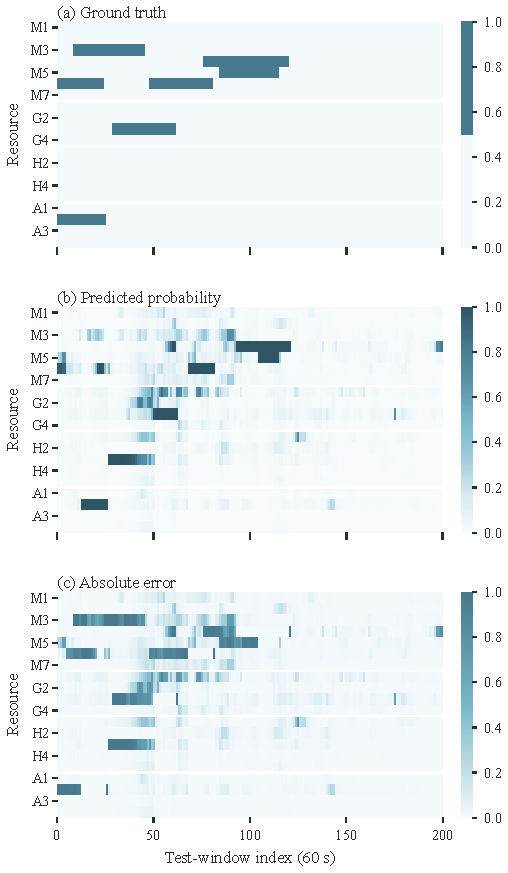
\includegraphics[width=\columnwidth]{figures/attention_heatmaps/fig08_prediction_heatmaps.pdf}
\caption{Future-event labels, predicted probabilities, and absolute errors for a mixed-condition episode (Start$\leq5$).}
\label{fig:attn-prediction}
\end{figure}

\paragraph*{Resource-level coverage.}
The overall Start$\leq5$ event F1-score is $80.4\%$, using the same onset-qualified matching criterion as Table~\ref{tab:comparison-main}. Table~\ref{tab:complete-6-1} retains the individual resource counts, F1-score, and duration errors behind the case analysis. It shows which workstations and handling resources contribute to the aggregate result; \texttt{robot\_2} and \texttt{robot\_3} have zero true events and are omitted.

\zhpara{\paragraph*{资源级覆盖。} 在 Start$\leq5$ 下，总体事件 F1-score 为 $80.4\%$，匹配准则与表~\ref{tab:comparison-main}相同。表~\ref{tab:complete-6-1}保留案例分析背后的逐资源计数、F1-score 与持续时间误差，说明哪些工位与搬运资源贡献了总体结果；\texttt{robot\_2} 与 \texttt{robot\_3} 无真实事件，故省略。}

% Author confirms overall F1 = 80.4 percent and the same matching criterion as the main table.
% Per-device server exports are pending synchronization; do not infer replacement device counts from the aggregate score.
\begin{table*}[pos=!tbp]
\centering
\scriptsize
\setlength{\tabcolsep}{3pt}
\renewcommand{\arraystretch}{1.12}
\caption{Per-device event and duration performance at Start$\leq5$. Durations are in minutes. Zero-support resources (\texttt{robot\_2}, \texttt{robot\_3}) are omitted.}
\label{tab:complete-6-1}
\begin{tabularx}{\textwidth}{@{}lXXXXXXX@{}}
\toprule
Device & $n_{\mathrm{true}}$ & $n_{\mathrm{pred}}$ & $P$ & $R$ & F1-score & Dur MAE & Dur RMSE \\
\midrule
num00\_weld\_ws0 & 115 & 100 & 70.0\% & 60.9\% & 65.1\% & 5.31 & 7.11 \\
num00\_weld\_ws1 & 17 & 19 & 89.5\% & 100.0\% & 94.4\% & 1.54 & 2.76 \\
num01\_robotweld\_ws0 & 46 & 25 & 76.0\% & 41.3\% & 53.5\% & 6.04 & 7.56 \\
num02\_CNC$^\ast$\_ws0 & 301 & 343 & 76.7\% & 87.4\% & 81.7\% & 4.67 & 6.45 \\
num04\_groove\_ws0 & 20 & 27 & 55.6\% & 75.0\% & 63.8\% & 5.32 & 6.87 \\
num08\_bench\_ws0 & 186 & 162 & 91.4\% & 79.6\% & 85.1\% & 3.47 & 5.02 \\
num08\_bench\_ws1 & 94 & 101 & 93.1\% & 100.0\% & 96.4\% & 2.65 & 3.65 \\
gantry\_0 & 18 & 26 & 57.7\% & 83.3\% & 68.2\% & 3.35 & 4.85 \\
gantry\_1 & 31 & 34 & 76.5\% & 83.9\% & 80.0\% & 4.55 & 6.45 \\
gantry\_2 & 108 & 132 & 74.2\% & 90.7\% & 81.7\% & 3.59 & 5.56 \\
gantry\_3 & 121 & 127 & 81.1\% & 85.1\% & 83.1\% & 3.56 & 5.04 \\
robot\_0 & 15 & 10 & 90.0\% & 60.0\% & 72.0\% & 4.01 & 6.14 \\
robot\_1 & 30 & 28 & 82.1\% & 76.7\% & 79.3\% & 5.03 & 6.80 \\
\bottomrule
\end{tabularx}
\end{table*}


\subsection{Prediction quality and computational cost}\label{sec:efficiency}

This experiment evaluates the computation required to deliver the predictive quality reported in Section~\ref{sec:comparison-event}. All five models perform inference on an NVIDIA GeForce RTX~5090. The environment uses Python~3.11.15 and CUDA~12.8, with PyTorch~2.11.0 for the neural models and XGBoost~3.2.0 with CuPy~14.2.0 for the seven tree-based prediction heads. Throughput is measured over five complete test passes at batch size 16 after 50 warm-up batches. Forward and report latency use batch size 1 and 5,000 timed calls, with CUDA synchronization before and after each measurement. The timing boundary covers model-side reporting. Forward timing covers prediction with inputs or prepared features resident on the GPU. Report timing includes input transfer, model-specific feature processing, prediction, and event-report generation; for XGBoost, this includes CPU history-feature construction, host-to-device transfer, seven CUDA prediction heads, and device-to-host output transfer. Batched test passes also include data loading. Table~\ref{tab:efficiency} summarizes the three onset caps, and Figure~\ref{fig:quality-cost} relates report latency to the F1-score values in Table~\ref{tab:comparison-main}.

\zhpara{本实验考察实现第~\ref{sec:comparison-event}节预测质量所需的计算成本。五种模型均在 NVIDIA GeForce RTX~5090 上执行推理。软件环境采用 Python~3.11.15 和 CUDA~12.8，神经模型使用 PyTorch~2.11.0，七个树模型预测头使用 XGBoost~3.2.0 与 CuPy~14.2.0。吞吐量采用 batch size 16，在五十个预热 batch 后完成五次完整测试。纯前向与报告延迟采用 batch size 1，统计 5,000 次调用，并在每次计时前后执行 CUDA 同步。计时边界覆盖模型侧报告生成。纯前向计时覆盖输入或已构造特征驻留 GPU 时的模型预测。报告计时包含输入传输、模型对应的特征处理、预测及事件报告生成；其中，XGBoost 包含 CPU 端历史特征构造、主机到设备的传输、七个 CUDA 预测头以及输出回传。批量测试还包含数据加载。表~\ref{tab:efficiency}汇总三个起点范围的开销，图~\ref{fig:quality-cost}将报告延迟与表~\ref{tab:comparison-main}中的 F1-score 对应展示。}

% All 15 GPU timing rows are verified against isaac_factory@a5b6c92,
% including the original PHGST-DM report snapshots. B2 uses the 2026-10-24 CUDA run.
% See experiments/efficiency_comparison_2026-10-24.md for provenance and checks.
\begin{table*}[t]
\centering
\caption{Inference cost on the RTX~5090. Ranges give the minimum and maximum across Start $\leq5$, $\leq10$, and $\leq15$ min. Throughput uses batch size 16 and report latency uses batch size 1. GPU allocation is the PyTorch allocator peak.}
\label{tab:efficiency}
\footnotesize
\setlength{\tabcolsep}{3.3pt}
\renewcommand{\arraystretch}{1.15}
\begin{tabular*}{\FullWidth}{@{\extracolsep{\fill}}lrrrrrr@{}}
\toprule
Model & Parameters & \makecell{GPU allocation\\(MiB)} & \makecell{Throughput $\uparrow$\\(samples/s)} & \makecell{Report p50 $\downarrow$\\(ms)} & \makecell{Report p95 $\downarrow$\\(ms)} & \makecell{Report p99 $\downarrow$\\(ms)} \\
\midrule
\textbf{PHGST-DM} & 713,984 & 175.8 & 1,946\textendash{}1,987 & 4.72\textendash{}4.77 & 5.32\textendash{}5.41 & 5.51\textendash{}5.60 \\
XGBoost & \na & \na & 236\textendash{}323 & 39.29\textendash{}58.55 & 41.73\textendash{}60.86 & 52.81\textendash{}72.66 \\
LSTM & 752,867 & 83.8 & 8,547\textendash{}8,740 & 0.64\textendash{}0.65 & 1.14\textendash{}1.15 & 1.33\textendash{}1.35 \\
BTGCN & 274,339 & 240.3 & 6,881\textendash{}7,274 & 0.92\textendash{}0.95 & 1.48\textendash{}1.51 & 1.62\textendash{}1.66 \\
BSTAN & 287,267 & 239.7 & 6,584\textendash{}6,667 & 1.00\textendash{}1.03 & 1.54\textendash{}1.58 & 1.64\textendash{}1.68 \\
\bottomrule
\end{tabular*}
\par\vspace{3pt}
\begin{minipage}{\FullWidth}
\scriptsize
Timing runs use the source-recorded workloads on a shared server under the same unified 5,354-window re-evaluation as Section~\ref{sec:comparison-overview}. GPU allocation includes resident inference inputs. XGBoost uses its native CUDA allocator, so its PyTorch allocation is unavailable; its separately sampled NVML process peak is 662--670~MiB, including the CUDA context, libraries, and caches.
\end{minipage}
\end{table*}

\begin{figure*}[t]
\centering
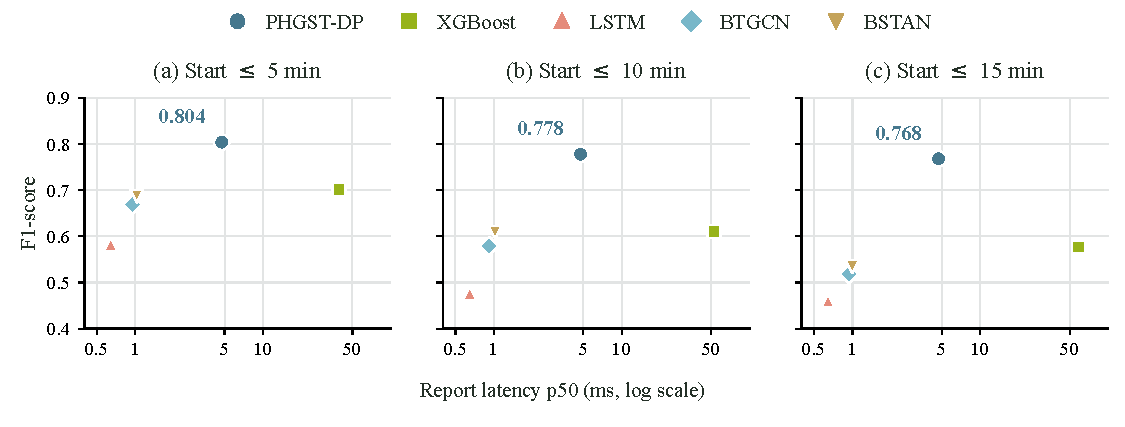
\includegraphics[width=0.96\textwidth]{figures/fig_quality_cost.pdf}
\caption{Event-identification quality versus median report latency for each onset cap.}
\label{fig:quality-cost}
\end{figure*}

PHGST-DM combines F1-score of $0.804/0.778/0.768$ with median report latency of 4.72--4.77~ms and p99 latency of 5.51--5.60~ms. Figure~\ref{fig:quality-cost} places it at the highest F1-score for each onset cap with millisecond-scale reporting. XGBoost's measured CUDA implementation has report p50 of 39.29--58.55~ms and p99 of 52.81--72.66~ms; LSTM, BTGCN, and BSTAN have median report latency below 1.1~ms. These measurements show the trade-off between predictive quality and report latency across the evaluated implementations. PHGST-DM's heterogeneous resource interactions and delay-aware modeling fit within a model-side reporting budget far shorter than the 60-s observation interval, making its event coverage and advance warning usable within the studied update cycle.

\zhpara{PHGST-DM 将 $0.804/0.778/0.768$ 的 F1-score 与 4.72--4.77~ms 的报告中位延迟、5.51--5.60~ms 的 p99 延迟结合起来。图~\ref{fig:quality-cost}中，模型在各起点范围保持最高的 F1-score，同时实现毫秒级报告生成。XGBoost CUDA 实现的实测报告 p50 为 39.29--58.55~ms、p99 为 52.81--72.66~ms；LSTM、BTGCN 和 BSTAN 的报告中位延迟低于 1.1~ms。这些工作点呈现被测实现的预测质量与运行成本选择。PHGST-DM 将异构资源交互和延迟感知建模纳入远短于六十秒观测间隔的模型侧报告预算，使事件覆盖与提前预警能够用于所研究的更新周期。}

The resource requirements remain stable across onset caps. PHGST-DM processes 1,946--1,987 samples/s, with a 0.05-ms spread in median report latency. Its 713,984 parameters occupy a 2.91-MiB checkpoint, and peak GPU allocation is approximately 175.8~MiB, about 27\% below BTGCN and BSTAN under the measured configurations; LSTM uses 83.8~MiB. The three checkpoints share the same architecture and input shape. This combination of a compact parameter set, stable inference cost, and detailed event predictions supports frequent report updates on the tested platform.

\zhpara{模型的资源需求在不同起点范围下保持稳定。PHGST-DM 的吞吐量为每秒 1,946--1,987 个样本，报告中位延迟的极差为 0.05~ms。模型包含 713,984 个参数，checkpoint 为 2.91~MiB，峰值 GPU allocated memory 约为 175.8~MiB，在被测配置下比 BTGCN 和 BSTAN 低约 $27\%$；LSTM 的相应占用为 83.8~MiB。三个 checkpoint 共享相同的架构和输入形状。紧凑的参数规模、稳定的推理成本与详细的事件预测共同支持在测试平台上频繁更新瓶颈报告。}

\section{Discussion}\label{sec:discussion}

The experiments show that PHGST-DM can combine advance warning with a detailed description of emerging bottlenecks in the evaluated multi-entity production environment. The baseline comparisons support improved event identification together with onset, duration, and production-state forecasting (Table~\ref{tab:comparison-main}), while the resource-level cases show how these outputs follow bottleneck onset, persistence, and recovery. Jointly reporting the affected resource, event interval, observable process cause, and remaining order time gives the forecast a production meaning beyond an isolated bottleneck score. The resulting contribution is an integrated description of where and when a constraint is expected, how long it may persist, and what operational context accompanies it.

\zhpara{实验表明，在所评估的多实体生产环境中，PHGST-DM 能够把提前预警与对新现瓶颈的详细描述结合起来。基线比较支持事件识别以及起点、持续时间和生产状态预测的改进（表~\ref{tab:comparison-main}）；资源级案例则展示这些输出如何跟随瓶颈的发生、持续与恢复。联合报告受影响资源、事件区间、可观测过程原因和订单剩余时间，使预报具有超出孤立瓶颈评分的生产含义。由此形成的贡献是对约束将出现在何处、何时、可能持续多久，以及伴随何种运行上下文的一体化描述。}

The component studies assess how the three methodological contributions affect predictive performance. First, the heterogeneous process--logistics graph allows the predictor to use workstation, worker, buffer, and transport information jointly. The graph and cross-resource ablations particularly affect upcoming-event recall, supporting the use of related-resource observations before a target becomes constrained (Table~\ref{tab:entity-ablation-new}). Second, process-informed supervision connects event and cause targets to observable production evidence, while temporal pattern clustering summarizes recurrent operating histories. The matched-budget cause study shows that the clearest benefit of cause supervision is improved process interpretation, with little change in station identification (Table~\ref{tab:matched-cause}). Third, delay-aware modeling uses the temporal-pattern context in cross-resource attention. Removing pattern matching reduces warning coverage for more distant onsets (Table~\ref{tab:delay-ablation-new}), supporting its predictive role in using lagged information. This evidence concerns forecast behaviour; it does not establish that attention recovers physical propagation paths or estimates actual propagation times.

\zhpara{组件研究评估三项方法贡献如何影响预测性能。第一，异构工艺—物流图使预测器能够联合利用工位、人员、缓冲与运输信息。图与跨资源消融尤其影响 Upcoming 召回率，支持在目标资源受限之前使用相关资源观测（表~\ref{tab:entity-ablation-new}）。第二，过程知情监督将事件与原因目标连接到可观测生产证据，时间模式聚类则归纳重复运行历史。匹配预算的原因研究表明，原因监督的最清晰收益是改进过程解释，而对工位识别影响很小（表~\ref{tab:matched-cause}）。第三，延迟感知建模在跨资源注意力中使用时间模式上下文。去掉原型匹配会降低较远起点事件的预警覆盖（表~\ref{tab:delay-ablation-new}），支持其在利用滞后信息方面的预测作用。上述证据针对预报行为，并不表明注意力恢复了物理传播路径或估计了实际传播时延。}

The report outputs can inform complementary production decisions. Resource and onset forecasts help determine where and when to direct attention; duration estimates help assess the available intervention window; process-cause outputs suggest conditions to inspect; and remaining-time estimates provide context for order-progress assessment. The model-side latency results support updating these reports within the studied one-minute observation cycle (Section~\ref{sec:efficiency}). A deployment interface could map observations from manufacturing execution systems (MES), warehouse management systems (WMS), and transport-dispatch systems to the resource graph, consistent with integrated monitoring and simulation platforms for reconfigurable manufacturing systems~\cite{leng2023monitoring}. Whether such information improves scheduling or throughput depends on the intervention policy and available resources and requires separate closed-loop evaluation.

\zhpara{报告输出可为互补的生产决策提供信息。资源与起点预报有助于判断应在何处、何时投入关注；持续时间估计有助于评估可用干预窗口；过程原因输出提示应检查的条件；剩余时间估计则为订单进度评估提供上下文。模型侧延迟结果表明，这些报告可在所研究的一分钟观测周期内更新（第~\ref{sec:efficiency}节）。部署接口可将制造执行系统（MES）、仓储管理系统（WMS）与运输调度系统的观测映射到资源图，这与可重构制造系统中的集成监测与仿真平台相一致~\cite{leng2023monitoring}。此类信息是否改善调度或吞吐量，取决于干预策略与可用资源，需要单独的闭环评估。}

The current evaluation uses an open-workspace factory environment developed for NVIDIA Isaac Sim. Transfer across layouts, products, and physical factories remains to be evaluated. Future work will extend validation to physical production systems and closed-loop resource interventions, examining how the forecasts support production decisions and measurable performance improvements.

\zhpara{当前评估基于面向 NVIDIA Isaac Sim 开发的开放式工厂环境。跨布局、跨产品与实体工厂的迁移仍有待检验。未来工作将把验证扩展到实体生产系统与闭环资源干预，考察预报如何支持生产决策并带来可度量的绩效改进。}

\section{Conclusion}\label{sec:conclusion}

This study presents PHGST-DM for dynamic bottleneck prediction in multi-entity production systems. A heterogeneous process--logistics graph broadens the observed resource interactions, process-informed supervision and temporal pattern clustering organize event targets and recurrent operating context, and delay-aware modeling uses historical cross-resource information for prediction. Experiments in the evaluated factory environment show improved event-prediction accuracy relative to the compared baselines, while ablations and production traces support the roles of these components in advance warning and temporal tracking. By jointly reporting bottleneck station, onset, duration, observable process cause, and remaining order time, PHGST-DM provides detailed forecasts that can inform timely resource interventions. Further validation in physical production systems is needed to determine whether these forecasts improve intervention decisions and production outcomes.

\zhpara{本文提出面向多实体生产系统动态瓶颈预测的 PHGST-DM。异构工艺—物流图扩展了可观测资源交互，过程知情监督与时间模式聚类组织事件目标与重复运行上下文，延迟感知建模利用历史跨资源信息进行预测。在所评估工厂环境中的实验表明，相对对照基线，事件预测精度有所提升；消融与生产轨迹进一步支持这些组件在提前预警与时间跟踪中的作用。通过联合报告瓶颈工位、起点、持续时间、可观测过程原因和订单剩余时间，PHGST-DM 提供可支持及时资源干预的详细预报。仍需在实体生产系统中进一步验证这些预报能否改进干预决策与生产结果。}

\printcredits

\section*{Declaration of Competing Interest}
The authors declare that they have no known competing financial interests or personal relationships that could have appeared to influence the work reported in this paper.

\section*{Data availability}
Data will be made available on request.

\section*{Acknowledgments}
The work described in this paper is supported by grants from RGC General Research Fund (17206126), Technology Cooperation Funding Scheme (TCFS) (Ref No.\ GHP/321/22SZ), The University of Hong Kong (Ref No.\ 2407102267, 2503252159), and Innovation and Technology Fund (ITF) (Ref No.\ TP/041/24LP).

%% Bibliography precedes the appendix, following common Elsevier layout.
\bibliographystyle{unsrtnat}
\bibliography{../cas-refs}

\clearpage
\appendix
\onecolumn
\section{Implementation Details and Additional Results}\label{app:additional}

This appendix provides implementation settings, numerical label and decoding rules, and the attention matrices underlying the main-text analysis.

\zhpara{本附录给出实现设置、数值标签与解码规则，以及支撑正文分析的注意力矩阵。}

Table~\ref{tab:shared-training-protocol} summarizes the settings shared by the Full model and ablation arms; their architectural differences are listed in Table~\ref{tab:ablation-arms}.

\zhpara{表~\ref{tab:shared-training-protocol}汇总 Full 模型与各消融分支的共用设置；架构差异见表~\ref{tab:ablation-arms}。}

\begin{table}[pos=htbp]
\centering
\caption{Shared training, model, and task settings for the Full model and ablation arms.}
\label{tab:shared-training-protocol}
\footnotesize
\setlength{\tabcolsep}{6pt}
\renewcommand{\arraystretch}{1.05}
\begin{tabularx}{\textwidth}{@{}lX@{}}
\toprule
Item & Setting \\
\midrule
Initialization and seed & Identical initial parameter values across arms; seed 42 \\
Optimizer and batch size & AdamW; batch size 16; weight decay 0.05 \\
Learning rate & $5\times10^{-5}$ initially; cosine decay to $10^{-6}$ \\
Sampling and training budget & Fourfold positive-window oversampling; at most 50 epochs per Start-cap run; early-stopping patience 40 \\
Curriculum & Start$\leq5\rightarrow$Start$\leq10\rightarrow$Start$\leq15$ \\
Checkpoint criterion & Validation station-identification F1 among candidates with report precision $\geq0.80$ and recall $\geq0.70$ \\
Threshold candidates & $\{0.45,0.50,0.55,0.60,0.65,0.70,0.75,0.80,0.85,0.88,0.90,0.94\}$ \\
Held-out evaluation & Freeze the selected checkpoint and threshold before evaluating the shared test episodes \\
Windowing and targets & 60-s windows; 30 historical and 30 future windows; seven workstation, four gantry, and four transport-robot targets \\
Event and matching rules & Eight-window persistence; one-window internal gap filling; Start$\leq5/10/15$; three-window onset tolerance \\
Encoder and attention & Five blocks; hidden dimension 80; temporal/geographic/semantic heads $4/2/2$ \\
Graph and positional context & Geographic hop cutoff 4; five semantic neighbours; eight-dimensional Laplacian encoding \\
Pattern bank & 16 prototypes from length-three temporal patches \\
Far-onset enhancement & Onset-loss multiplier 2; positive weights $9/10/11$ for Start$\leq5/10/15$ \\
False-alarm weighting & Ordinary false-positive weight 2.5; additional hard-false-positive multiplier 2.2 \\
\bottomrule
\end{tabularx}
\end{table}

The objective in Section~\ref{sec:method} uses the following weights. Event occurrence, start, duration, and prefix losses have weights $2.4$, $2.0$, $2.0$, and $2.5$, respectively. The cold-history onset term has weight $2.2$ within the event-occurrence objective; focal modulation uses exponent $1.5$, and the internal differentiable F1 term has weight $0.8$. Future occupancy uses separate binary-cross-entropy, Dice, and IoU weights of $0.7$, $0.5$, and $0.35$. The reconstruction, supervised contrastive, cause, and turning-point/momentary losses have weights $0.2$, $0.05$, $0.1$, and $0.25$. Remaining-time regression has weight $0.5$ in stage~1 and $4.0$ during head-only stage~2.

\zhpara{\paragraph{补充实现参数。}
\label{app:implementation-parameters}
该配置对第~\ref{sec:method}节目标作如下扩展。事件发生、起点、持续时间和前缀损失权重分别为 $2.4$、$2.0$、$2.0$ 和 $2.5$。冷历史起点项在事件发生目标中权重为 $2.2$；focal 调制指数为 $1.5$，内部可微 F1 项权重为 $0.8$。未来占用的二元交叉熵、Dice 与 IoU 权重分别为 $0.7$、$0.5$ 和 $0.35$。重构、监督对比、原因以及转折点/瞬时损失权重分别为 $0.2$、$0.05$、$0.1$ 和 $0.25$。剩余时间回归在阶段~1 权重为 $0.5$，在仅微调头的阶段~2 为 $4.0$。遗留评分、will、mark、到起点时间、STGNPP 与离线聚类目标权重均为零。这些系数区分了现行事件发生损失与已停用的遗留 will 目标。}

All state rules act on the original physical feature scale before input standardization. Let $q$, $B$, $S$, $U$, $I$, $R$, and $Z$ denote queue length, blocked seconds, starved seconds, unavailable fraction, inbound-wait seconds, route-delay seconds, and shortage propagation, respectively. At the 60-s resolution, a workstation has raw hot evidence if any of the following holds: (i) $q\geq2$ and $B+S>0$; (ii) $B\geq24$ and $q\geq1$; (iii) $B+S\geq24$ together with an upstream/downstream coupling ratio of at least $0.15$, $I\geq20$, $R\geq20$, $Z\geq0.25$, or $q\geq1$; (iv) $S\geq30$ and $Z\geq0.25$; (v) $S\geq18$ and either $I\geq20$ or $R\geq20$; or (vi) $B+S\geq24$ together with worker absence or labour saturation. An active workstation operating-variation flag combined with $U\geq0.5$ also supplies hot evidence. Worker absence uses unavailable fraction $\geq0.5$; labour saturation uses an activity cutoff of $0.8$ among present workers, with a presence tolerance of $0.05$. A gantry requires $B+S\geq18$ and either $I\geq20$ or $R\geq20$, whereas a transport robot requires $B+S\geq18$ and $I\geq20$; either handling type is also hot when $U\geq0.5$. When an operating-variation flag is active, evidence is retained only if $q\geq1$, $B+S\geq24$, or $U\geq0.5$. The eight-window removal and one-window internal-gap rule are then applied as described in Algorithm~\ref{alg:targets}.

\zhpara{\paragraph{数值运行状态阈值。}
全部状态规则作用于输入标准化之前的原始物理特征尺度。记 $q$、$B$、$S$、$U$、$I$、$R$ 与 $Z$ 分别表示队列长度、阻塞秒数、饥饿秒数、不可用比例、入站等待秒数、路径延迟秒数与短缺传播。在 60~s 分辨率下，工位在满足下列任一条件时具有原始热点证据：(i) $q\geq2$ 且 $B+S>0$；(ii) $B\geq24$ 且 $q\geq1$；(iii) $B+S\geq24$，并同时满足上下游耦合比至少为 $0.15$、$I\geq20$、$R\geq20$、$Z\geq0.25$ 或 $q\geq1$；(iv) $S\geq30$ 且 $Z\geq0.25$；(v) $S\geq18$ 且 $I\geq20$ 或 $R\geq20$；或 (vi) $B+S\geq24$ 并伴随人员缺席或劳动力饱和。活动的工位运行变化标志与 $U\geq0.5$ 也可提供热点证据。人员缺席采用不可用比例 $\geq0.5$；劳动力饱和在在岗人员中采用活动阈值 $0.8$，在岗容差为 $0.05$。龙门要求 $B+S\geq18$ 且 $I\geq20$ 或 $R\geq20$；运输机器人要求 $B+S\geq18$ 且 $I\geq20$；任一搬运类型在 $U\geq0.5$ 时亦判定为热点。当运行变化标志激活时，仅在 $q\geq1$、$B+S\geq24$ 或 $U\geq0.5$ 时保留证据。随后按算法~\ref{alg:targets}应用八窗口剔除与一窗口内部间隙规则。}

The prefix-continuation cutoff is $1.5$ windows. Occupancy-run extraction for event union uses probability cutoff $0.45$, with both ongoing and upcoming union enabled; direct occupancy-state evaluation uses cutoff $0.55$. The configured gantry and transport-robot report thresholds are $0.72$ and $0.68$, respectively, alongside the validation-selected global operating point. Threshold selection first prefers candidates satisfying the validation precision requirement and then maximizes the configured station-identification F1; if none satisfies that requirement, it retains the highest-F1 validation candidate. The checkpoint precision/recall gates are applied separately. If no gated checkpoint is obtained throughout training, the retained ungated checkpoint with the best validation selection score is used. Neither fallback uses test predictions or test labels.

\zhpara{\paragraph{解码器与验证回退。}
前缀延续截断为 $1.5$ 个窗口。用于事件并集的占用段提取概率截断为 $0.45$，并同时启用进行中与即将发生并集；直接占用状态评价截断为 $0.55$。所配置的龙门与运输机器人报告阈值分别为 $0.72$ 与 $0.68$，并与验证选定的全局工作点并用。阈值选择先优先满足验证精确率要求，再最大化所配置的工位识别 F1；若不存在满足要求的候选，则保留验证 F1 最高者。检查点精确率/召回率门控单独施加。若训练全程未得到门控检查点，则使用验证选择分数最高的未门控检查点。两类回退均不使用测试预测或测试标签。}

Evaluation counts refer to forecast-origin--resource pairs, so a persistent event may contribute at successive origins. Overlapping windows are not treated as independent observations for significance testing.

\zhpara{评价计数按预报起点—资源对统计，因此持续事件可在多个相继起点上贡献。重叠窗口不作独立性假设下的显著性检验观测。}

\label{app:absolute-attention}
\label{app:layerwise-attention}
Figures~\ref{fig:attn-states} and~\ref{fig:attn-layers-all} give the absolute resource-attention averages and all five encoder layers underlying Figures~\ref{fig:attn-change} and~\ref{fig:attn-layers}. The resource matrices show 20 non-buffer resources without renormalization after omitting the 18 buffers. Layer-wise matrices share within-branch scales. Attention describes learned associations rather than causal effects or layer-wise accuracy contributions.

\clearpage
\begin{figure*}[!t]
\centering
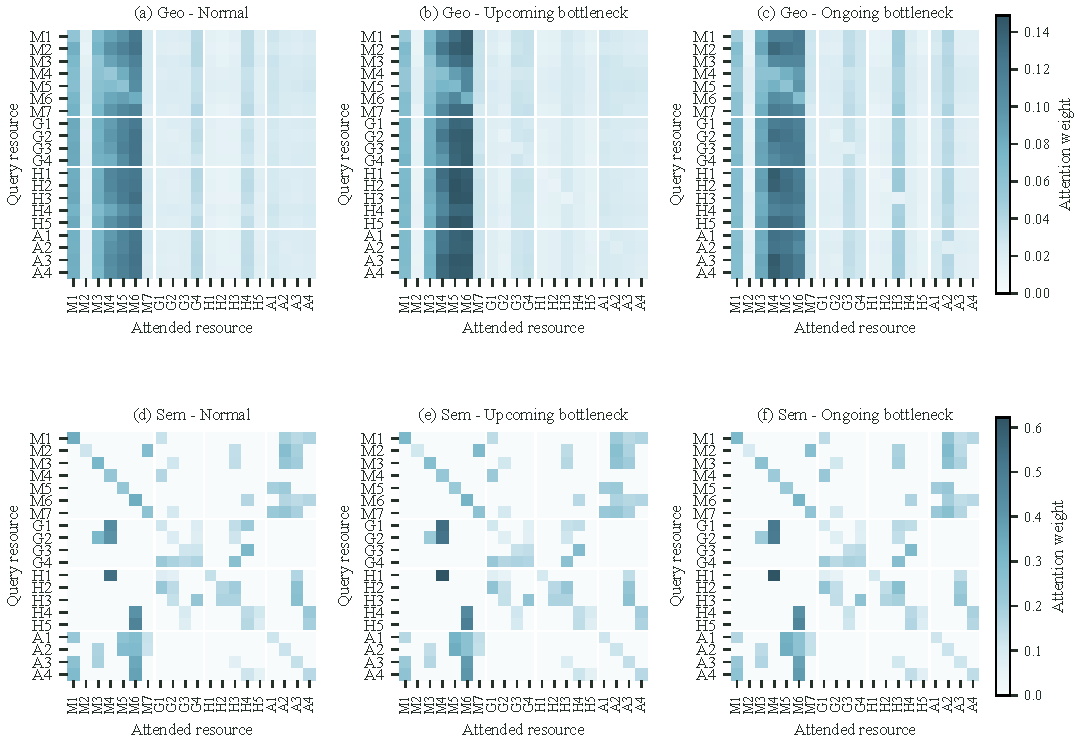
\includegraphics[width=0.92\textwidth]{figures/attention_heatmaps/fig02_resource_attention_states.pdf}
\caption{Absolute geographic (upper) and semantic (lower) resource attention under normal, upcoming, and ongoing conditions.}
\label{fig:attn-states}
\end{figure*}

\begin{figure*}[t]
\centering
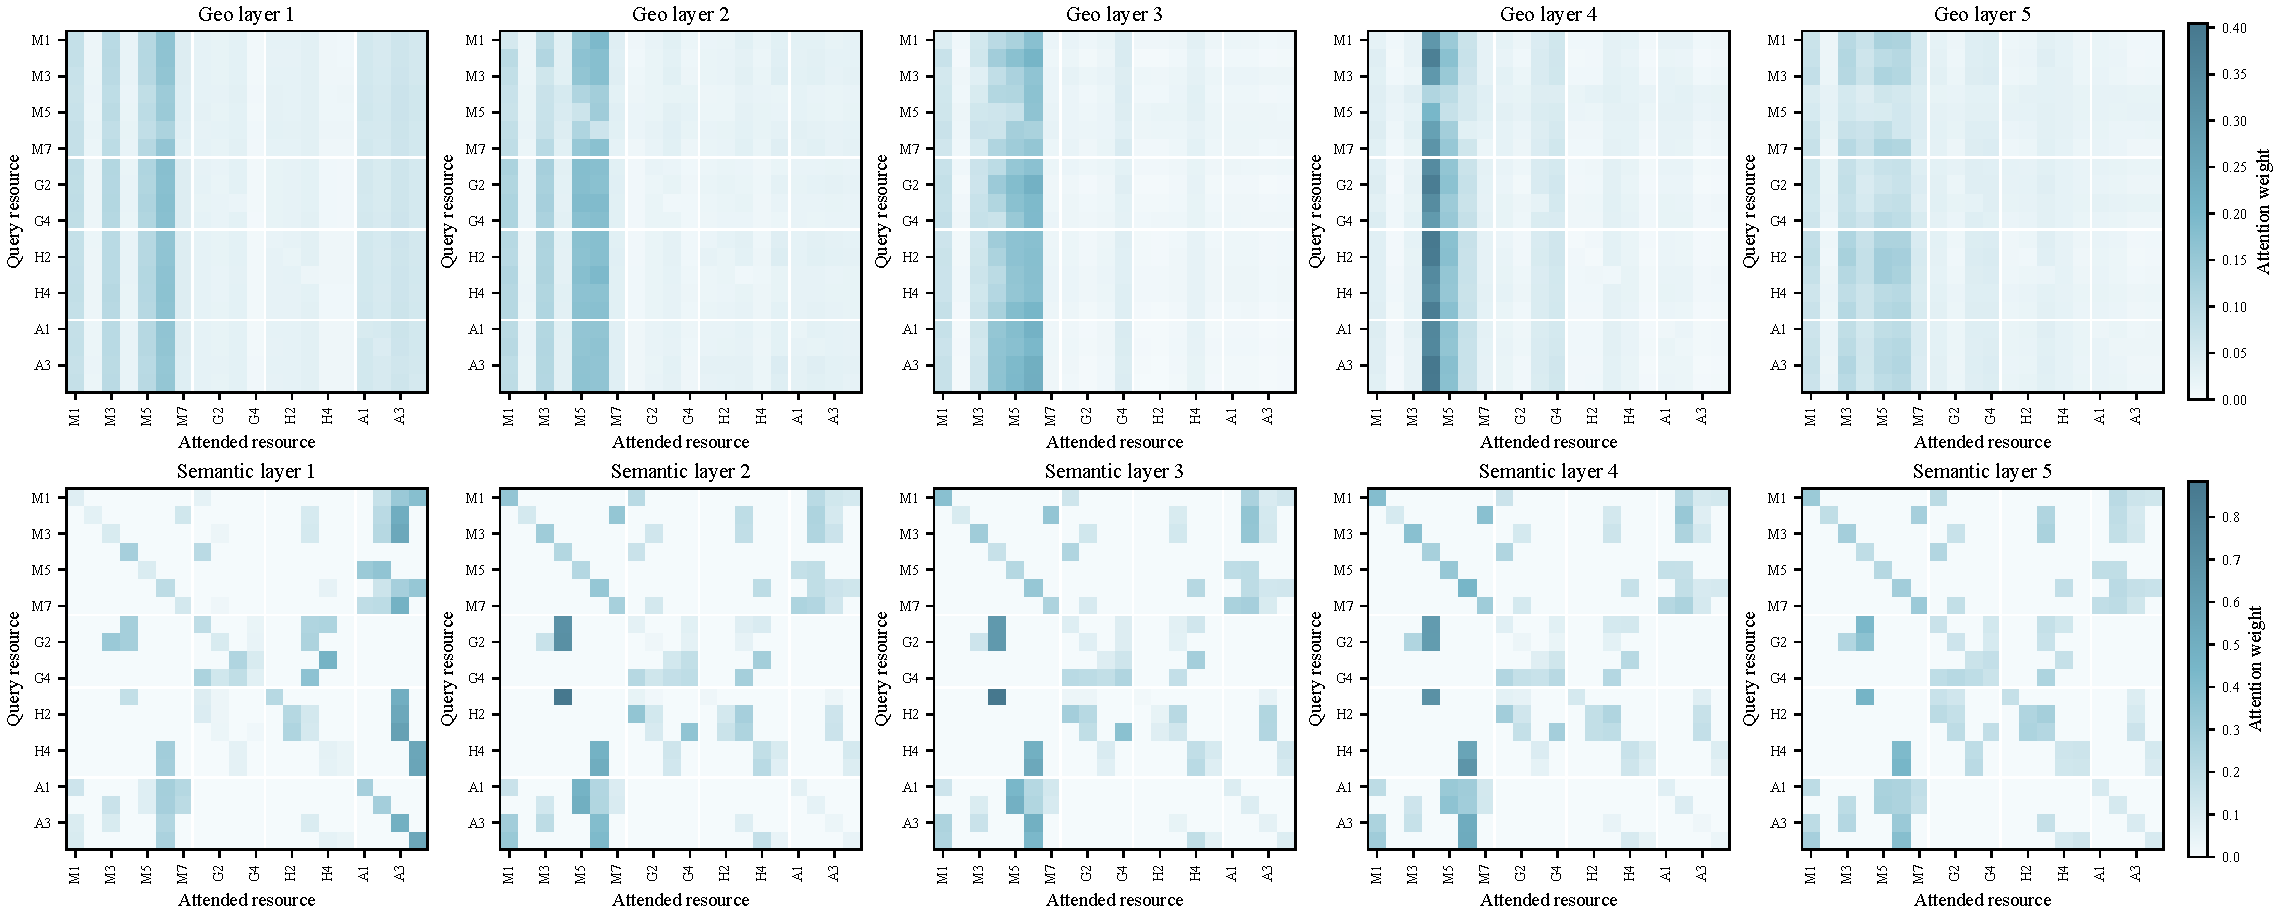
\includegraphics[width=0.94\textwidth]{figures/attention_heatmaps/fig05_layerwise_upcoming_attention.pdf}
\caption{Geographic (upper) and semantic (lower) attention across encoder layers 1--5 for upcoming samples.}
\label{fig:attn-layers-all}
\end{figure*}

\end{document}
